% Options for packages loaded elsewhere
\PassOptionsToPackage{unicode}{hyperref}
\PassOptionsToPackage{hyphens}{url}
%
\documentclass[
  man,floatsintext]{apa6}
\usepackage{lmodern}
\usepackage{amssymb,amsmath}
\usepackage{ifxetex,ifluatex}
\ifnum 0\ifxetex 1\fi\ifluatex 1\fi=0 % if pdftex
  \usepackage[T1]{fontenc}
  \usepackage[utf8]{inputenc}
  \usepackage{textcomp} % provide euro and other symbols
\else % if luatex or xetex
  \usepackage{unicode-math}
  \defaultfontfeatures{Scale=MatchLowercase}
  \defaultfontfeatures[\rmfamily]{Ligatures=TeX,Scale=1}
\fi
% Use upquote if available, for straight quotes in verbatim environments
\IfFileExists{upquote.sty}{\usepackage{upquote}}{}
\IfFileExists{microtype.sty}{% use microtype if available
  \usepackage[]{microtype}
  \UseMicrotypeSet[protrusion]{basicmath} % disable protrusion for tt fonts
}{}
\makeatletter
\@ifundefined{KOMAClassName}{% if non-KOMA class
  \IfFileExists{parskip.sty}{%
    \usepackage{parskip}
  }{% else
    \setlength{\parindent}{0pt}
    \setlength{\parskip}{6pt plus 2pt minus 1pt}}
}{% if KOMA class
  \KOMAoptions{parskip=half}}
\makeatother
\usepackage{xcolor}
\IfFileExists{xurl.sty}{\usepackage{xurl}}{} % add URL line breaks if available
\IfFileExists{bookmark.sty}{\usepackage{bookmark}}{\usepackage{hyperref}}
\hypersetup{
  pdftitle={What measure of effect size when comparing two groups based on their means?},
  pdfauthor={Marie Delacre~\& Christophe Leys},
  pdfkeywords={keywords},
  hidelinks,
  pdfcreator={LaTeX via pandoc}}
\urlstyle{same} % disable monospaced font for URLs
\usepackage{longtable,booktabs}
% Correct order of tables after \paragraph or \subparagraph
\usepackage{etoolbox}
\makeatletter
\patchcmd\longtable{\par}{\if@noskipsec\mbox{}\fi\par}{}{}
\makeatother
% Allow footnotes in longtable head/foot
\IfFileExists{footnotehyper.sty}{\usepackage{footnotehyper}}{\usepackage{footnote}}
\makesavenoteenv{longtable}
\usepackage{graphicx,grffile}
\makeatletter
\def\maxwidth{\ifdim\Gin@nat@width>\linewidth\linewidth\else\Gin@nat@width\fi}
\def\maxheight{\ifdim\Gin@nat@height>\textheight\textheight\else\Gin@nat@height\fi}
\makeatother
% Scale images if necessary, so that they will not overflow the page
% margins by default, and it is still possible to overwrite the defaults
% using explicit options in \includegraphics[width, height, ...]{}
\setkeys{Gin}{width=\maxwidth,height=\maxheight,keepaspectratio}
% Set default figure placement to htbp
\makeatletter
\def\fps@figure{htbp}
\makeatother
\setlength{\emergencystretch}{3em} % prevent overfull lines
\providecommand{\tightlist}{%
  \setlength{\itemsep}{0pt}\setlength{\parskip}{0pt}}
\setcounter{secnumdepth}{-\maxdimen} % remove section numbering
\shorttitle{Effect size}
\affiliation{
\vspace{0.5cm}
\textsuperscript{1} Université Libre de Bruxelles, Service of Analysis of the Data (SAD), Bruxelles, Belgium}
\keywords{keywords\newline\indent Word count: X}
\usepackage{csquotes}
\usepackage{upgreek}
\captionsetup{font=singlespacing,justification=justified}

\usepackage{longtable}
\usepackage{lscape}
\usepackage{multirow}
\usepackage{tabularx}
\usepackage[flushleft]{threeparttable}
\usepackage{threeparttablex}

\newenvironment{lltable}{\begin{landscape}\begin{center}\begin{ThreePartTable}}{\end{ThreePartTable}\end{center}\end{landscape}}

\makeatletter
\newcommand\LastLTentrywidth{1em}
\newlength\longtablewidth
\setlength{\longtablewidth}{1in}
\newcommand{\getlongtablewidth}{\begingroup \ifcsname LT@\roman{LT@tables}\endcsname \global\longtablewidth=0pt \renewcommand{\LT@entry}[2]{\global\advance\longtablewidth by ##2\relax\gdef\LastLTentrywidth{##2}}\@nameuse{LT@\roman{LT@tables}} \fi \endgroup}


\usepackage{lineno}

\linenumbers
\usepackage{rotating}
\DeclareDelayedFloatFlavor{sidewaysfigure}{figure}

\title{What measure of effect size when comparing two groups based on their means?}
\author{Marie Delacre\textsuperscript{1}~\& Christophe Leys\textsuperscript{1}}
\date{}

\authornote{

Correspondence concerning this article should be addressed to Marie Delacre, CP191, avenue F.D. Roosevelt 50, 1050 Bruxelles. E-mail: \href{mailto:marie.delacre@ulb.ac.be}{\nolinkurl{marie.delacre@ulb.ac.be}}}

\abstract{

}

\begin{document}
\maketitle

\hypertarget{intro}{%
\section{Intro}\label{intro}}

During decades, researchers in social science (Henson \& Smith, 2000) and education (Fan, 2001) have overestimated the ability of the null hypothesis (H0) testing to determine the importance of their results. The standard for researchers in social science is to define H0 as the absence of effect (Meehl, 1990). For example, when comparing the mean of two groups, researchers commonly test the H0 that there is no mean differences between groups (Steyn, 2000). Any effect that is significantly different from zero will be seen as sole support for a theory.

Such an approach has faced many criticisms among which the most relevant to our concern is that the null hypothesis testing highly depends on sample size: for a given alpha level and a given difference between groups, the larger the sample size, the higher the probability of rejecting the null hypothesis (Fan, 2001; Kirk, 2009; Olejnik \& Algina, 2000; Sullivan \& Feinn, 2012). It implies that even tiny differences could be detected as statistically significant with very large sample sizes (McBride, Loftis, \& Adkins, 1993)\footnote{Tiny differences might be due to sampling error, or to other factors than the one of interest: even under the assumption of random assignent (which is a necessary but not sufficient condition), it is almost impossible to be sure that the only difference between two conditions is the one defined by the factor of interest. Other tiny factors of no theoretical interest might slighly influence results, making the probability of getting an actual zero effect very low. This is what Meehl (1990) calls 'systematic noise'.}.

Facing this argument, it has become an adviced practice to report the \emph{p}-value assorted by a measure of the effect size, that is, a quantitative measure of the magnitude of the experimental effect (Cohen, 1965; Fan, 2001; Hays, 1963). This practice is also highly endorsed by the American Psychological Association (APA) and the American Educational Research Association (AERA) (American Educational Research Association, 2006; American Psychological Association, 2010). However, limited studies properly report effect size in the last several decades.

Generally, there is a high confusion between the effect size and other related concepts such as the Applied significance\footnote{In our conception  Applied significance" encompass all what refers to the relevance of an effect in real life, e.g. clinical, personnal, social, professionnal.}. Moreover, there are several situations that call for effect size measures and in the current litterature, it's not always easy to know which measure using in a specific context. We will therefore introduce this paper with 3 sections in which we will:\\
1. Clearly define what is a measure of effect size;\\
2. Listing the different situations that call for effect sizes measure;\\
3. Define required properties of the effect size estimators, as a function of the situations.

Moreover, it is highly recommended to compute a confidence interval around the point effect size. In a fourth section, we will therefore summarize how it is an added value to mention the confidence interval around the effect size.

After these general adjustments, we will focus our attention on \enquote{between-subject} designs where individuals are randomly assigned into one of two independant groups and groups scores are compared based on their means\footnote{We made this choice because *t*-tests are still the most commonly used tests in the field of Psychology.}. Because it has been widely argued that there are many fields in psychology where the assumption of equal variances between two populations is ecologically unlikely (Delacre, Lakens, \& Leys, 2017; Erceg-Hurn \& Mirosevich, 2008; Grissom, 2000), it is becoming more common in statistical software to present a \emph{t}-test that does not hold on this assumption by default, namely the Welch's \emph{t}-test (e.g., R, Minitab). However, similar issues for the measures of effect sizes has received less attention (Shieh, 2013), and Cohen's \(d_s\) remains persistent\footnote{For example, in Jamovi, Cohen's ds is provided, whatever one performs Student's or Welch's t-test.}. One possible reason is that researchers cannot find a consensus on which alternative should be in use (Shieh, 2013). We will limit our study to the standardized mean difference, called the \emph{d}-family, because it is the dominant family of estimators of effect size when comparing two groups based on their means (Peng, Chen, Chiang, \& Chiang, 2013; Shieh, 2013), and we will see that even in this very specific context, there is little agreement between researchers as to which is the most suitable estimator. According to us, the main reason is that it is difficult, based on currently existing measures, to optimally serves all the purposes of en affect size measure. Throughout this section, we will:\\
1. Present the main measures of the \emph{d}-family that are proposed in the literature,related to the purpose they serve, and introduce a new one, namely the \enquote{transformed Shieh's \emph{d}} that should help at reaching all the purposes simultaneously;\\
2. Present and discuss the results of simulations we performed, in order to compare existing measures and the new introduced one;\\
3. Summarize our conclusions in practical recommandations. In this section, we will provide useful tools (i.e.~R package) to compute relevant measures of effect sizes and related information.

\hypertarget{measure-of-effect-size-what-it-is-what-it-is-not}{%
\section{Measure of effect size: what it is, what it is not}\label{measure-of-effect-size-what-it-is-what-it-is-not}}

The effect size is commonly refered to the practical significance of a test. Grissom \& Kim (2005) define the effect size as the extent to which results differ from what is implied by the null hypothesis. In the context of the comparison of two groups based on their mean, depending on the defined null hypothesis (considering the absence of effect as the null hypothesis), we could define the effect size either as the magnitude of differences between parameters of two populations groups are extracted from (e.g.~the mean; Peng \& Chen, 2014) or as the magnitude of the relation between one dichotomous factor and one dependent variable (American Educational Research Association, 2006). Both definitions refers to as the most famous families of measures of effect sizes (Rosenthal, 1994): respectively the \emph{d}-family and the \emph{r}-family.

Very often, the contribution of the measures of effect size is overestimated. First, benchmarks about what should be a small, medium or large effect size might have contribued at seeing the effect size as a measure of the importance or the relevance of an effect in real life, but it is not (Stout \& Ruble, 1995). The effect size is only a mathematical indicator of the magnitude of a difference, which depends on the way a variable is converted into numerical indicator. In order to assess the meaningfulness of an effect, we should be able to relate this effect with behaviors/meaningful consequences in the real world (Andersen, McCullagh, \& Wilson, 2007). For example, let us imagine a sample of students in serious school failure who are randomly divided into two groups: an experimental group following a training program and a control group. At the end of the training, students in the experimental group have on average significantly higher scores on a test than students in the control group, and the difference is large (e.g.~30 percents). Does it mean that students in the experimental condition will be able to pass to the next grade and to continue normal schooling? Whether the computed magnitude of difference is an important, meaningful change in everyday life refers to another construct that we will call the \emph{Applied significance}. It refers to the interpretation of treatment outcomes and is neither statistical nor mathematical, it is related to underlying theory that posits an empirical hypothesis. In other words, the relation between \emph{practical} and \emph{Applied} significance is more a theoretical argument than a statistical one.

Second, in the context of the comparison of two groups based on their means, it should not replace the null hypothesis testing. Statistical testing allows the researcher to determine whether the oberved departure from H0 occured by chance or not (Stout \& Ruble, 1995). while effect size estimators allow to assess the practical signficance of an effect, and as reminds Fan (2001): \emph{\enquote{a practically meaningful outcome may also have occured by chance, and consequently, is not trustworthy}} (p.278). For this reason, the use of confidence intervals around the effect size estimate is highly recommended (Bothe \& Richardson, 2011).

\hypertarget{different-purposes-of-effect-size-measures}{%
\section{Different purposes of effect size measures}\label{different-purposes-of-effect-size-measures}}

Effect size measures can be used in an \emph{inferential} perspective:\\
- The effect sizes from previous studies can be used in a priori power analysis when planning a new study (Lakens, 2013; Prentice \& Miller, 1990; Stout \& Ruble, 1995; Sullivan \& Feinn, 2012; Wilkinson \& the Task Force on Statistical Inference, 1999);\\
- We can also compute confidence limits around the point estimator (Shieh, 2013), in order to replace conventional hypothesis testing : if the null hypothesis area is out of the confidence interval, we can conclude that the null hypothesis is false.

Measures of effect size can also be used in a \emph{comparative} perspective, that is to assess the stability of results across designs, analysis, samples sizes (Wilkinson \& the Task Force on Statistical Inference, 1999). It includes:\\
- To compare results of 2 or more studies (Prentice \& Miller, 1990);\\
- To incorporate results in meta-analysis (Lakens, 2013; Li, 2016; Nakagawa \& Cuthill, 2007; Stout \& Ruble, 1995; Wilkinson \& the Task Force on Statistical Inference, 1999).

Finally, effect size measures can be used for \emph{interpretative} purposes: in order to assess the practical significance of a result (beyond statistical significance; Lakens, 2013; American Psychological Association, 2010; Prentice \& Miller, 1990).

\hypertarget{properties-of-a-good-effect-size-estimator}{%
\section{Properties of a good effect size estimator}\label{properties-of-a-good-effect-size-estimator}}

The estimate of an estimator depends on the sampling. That is to say, based on different samples extracted from the same population, one would obtain different estimates of the same estimator. The \emph{sampling distribution} of the estimator is the distribution of all estimates, based on all possible samples of size \emph{n} extracted from one population. Studying the sampling distribution is very useful, as it allows to assess the goodness of an effect size estimator and more specifically, three desirable properties of a good estimator for inferential purposes: \textbf{unbiasedness}, \textbf{consistency} and \textbf{efficiency} (Wackerly, Mendenhall, \& Scheaffer, 2008).

An estimator is unbiased if the distribution of estimates is centered around the true population parameter. On the other hand, an estimator is positively (or negatively) biased if the distribution is centered around a value that is higher (or smaller) than the true population parameter (see Figure \ref{fig:BIAS}). In other words, the bias tells us if estimates are good, on average. The \emph{bias} of a point estimator \(\hat{\delta}\) can be computed as follows:

\begin{equation} 
\hat{\delta}_{bias}=E(\hat{\delta})-\delta
\label{eq:BIAS}
\end{equation}

Where \(E(\hat{\delta})\) is the expectency of the sampling distribution of the estimator (i.e.~the average estimate) and \(\delta\) is the true parameter.

\begin{figure}
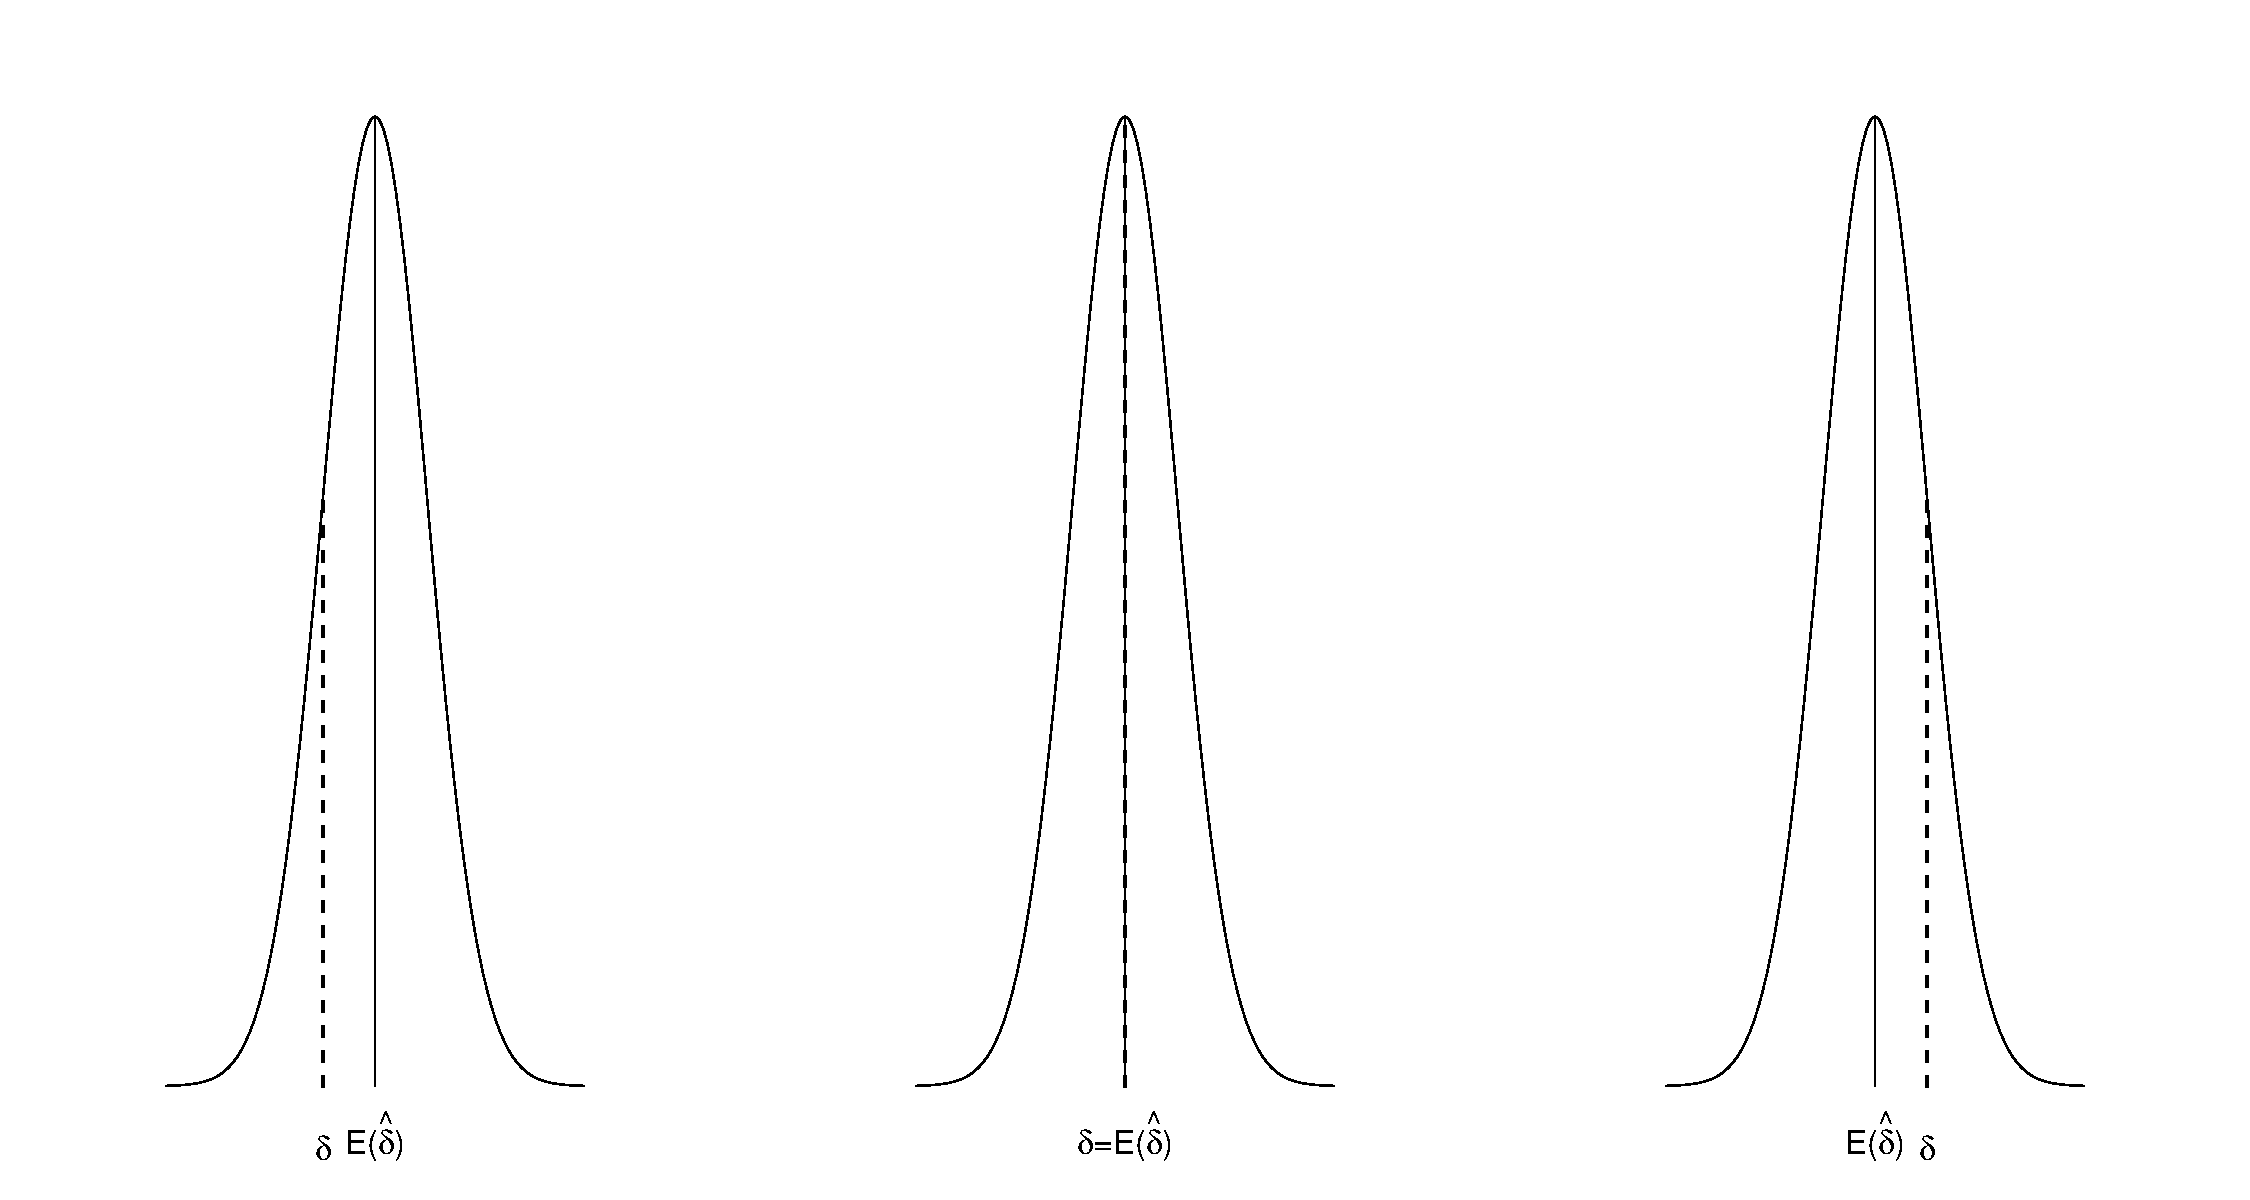
\includegraphics[width=400px]{ES_files/figure-latex/BIAS-1} \caption{Samplig distribution for a positively biased (left), an unbiased (center) and a negatively biased estimator (right)}\label{fig:BIAS}
\end{figure}

Moreover, since there is a strong relationship between the bias and the size of any estimator (the larger an estimator, the larger the bias), it might be interesting to also define the \emph{relative bias} as the ratio between the bias and the population estimator:

\begin{equation} 
\hat{\delta}_{relative \; bias}=\frac{E(\hat{\delta})-\delta}{\delta}
\label{eq:RELBIAS}
\end{equation}

Bias informs us about the goodness of estimates averages, but says nothing about individual estimates. Imagine a situation where the distribution of estimates is centered around the real parameter but with such a large variance that some point estimates are very far from the center. It would be problematic, as long as we have only one estimate, the one based on our sample, and we don't know how far is this estimate from the center of the sampling distribution. We hope that \emph{all} possible estimates are close enough of the true population parameter, in order to be sure that for \emph{any} estimate, one has a correct estimation of the real parameter. In other words, we expect the variability of estimates around the true population parameter to be as small as possible. It refers to the \textbf{efficiency} of the point estimator and can be computed as follows:

\begin{equation} 
\hat{\delta}_{efficiency}=Var(\hat{\delta})
\label{eq:EFFICIENCY}
\end{equation}

Where \(Var(\hat{\delta})\) is the variance of the sampling distribution of the estimator. Among all unbiased estimators, the more efficient will be the one with the smallest variance. Again, the variance of an estimator is a function of its size (the larger the estimator, the larger the variance) and therefore, we might be interested in computing the \emph{relative variance} as the ratio between the variance and the square of the population estimator:

\begin{equation} 
\hat{\delta}_{relative \; variance}=\frac{Var(\hat{\delta})}{\delta^2}
\label{eq:RELBIAS}
\end{equation}

Note that both unbiasedness and efficiency are very important. An unbiased estimator with such a large variance that somes estimates are extremely far from the real parameter is as undesirable as a parameter which is highly biased. In some situations, it is better to have a very slightly biased estimator with a tigh shape around the biased value, so each estimate remains relatively close to the true parameter, than an unbiased estimator with a large variance (Raviv, 2014).

Finally, the last property of a good point estimator is \textbf{consistency}: consistency means that the bigger the sample size, the closer the estimate of the population parameter. In other words, the estimates \emph{converge} to the true population parameter.

Beyond the inferential properties, Cumming (2013) reminds that an effect size estimator need to have a constant value across designs in order to be easily interpretable and to be included in meta-analysis. In other word, it should achieve the property of \textbf{generality}.

\hypertarget{confidence-interval-around-a-point-estimator}{%
\section{Confidence interval around a point estimator}\label{confidence-interval-around-a-point-estimator}}

We already mentioned that confidence interval around a point estimate could replace conventional hypothesis testing. The Confidence interval delivers all the information that \(p\)-value does: if the null values are out of the confidence interval, it means that an hypothesis test would have resulted in a \emph{p}-value below the nominal alpha level. At the same time, it provides extra informations about the precision of the sample estimate for inferential purposes, and therefore on how confident we can be in the observed results (Altman, 2005; Ellis, 2015): the narrower the interval indicates, the higher the precision and the lower the incertainty. On the other hand, the wider the confidence interval, the more the data lacks precision (for example, because the sample size were too small).

\hypertarget{different-measures-of-effect-sizes}{%
\section{Different measures of effect sizes}\label{different-measures-of-effect-sizes}}

The \emph{d}-family effect sizes are commonly used with \enquote{between-subject} designs where individuals are randomly assigned into one of two independant groups and groups scores means are compared. The population effect size is defined as follows:

\begin{equation} 
\delta = \frac{\mu_{1}-\mu_{2}}{\sigma} 
\label{eq:Cohendelta}
\end{equation}

Where both populations follow a normal distribution with the mean \(\mu_j\) in the \(j^{th}\) population (j=1,2) and standard deviation \(\sigma\). They exist different estimators of this effect size measure varying as a function of the chosen standardizer (\(\sigma\)). For all estimators, the mean difference is estimated by the difference of both sample means (\(\bar{X}_1-\bar{X}_2\)). When used for inference, some of them rely on both assumptions of normally distributed residuals and equality of variances, while others rely solely on the normally distributed residuals assumption.

\hypertarget{alternatives-when-variances-are-equal-between-groups}{%
\subsection{Alternatives when variances are equal between groups}\label{alternatives-when-variances-are-equal-between-groups}}

The most common estimator of \(\delta\) is Cohen's \(d_{s}\) where the sample mean difference is divided by a pooled error term (Cohen, 1965):

\begin{equation} 
Cohen's \; d_s = \frac{\bar{X}_1-\bar{X}_2}{\sqrt{\frac{(n_1-1) \times SD_1+(n_2-1) \times SD_2}{n_1+n_2-2}}} 
\label{eq:Cohends}
\end{equation}

Where \(SD_j\) is the standard deviation of the \(j^{th}\) sample and \(n_j\), the sample size of the \(j^{th}\) sample (j=1,2). The reasoning behind this measure is that considering both samples as extracted from a common population variance (n.d.), we achieve a more accurate estimation of the population variance by pooling both estimates of this parameter (i.e \(SD_1\) and \(SD_2\)) and because the larger the sample size, the more accurate the estimate, we give more weight to the estimate based on the larger sample size. Unfortunately, even under the assumptions that residuals are independant and identically normally distributed with the same variance across groups, Cohen's \(d_s\) is known to be positively biased (Lakens, 2013) and for this reason, Hedges \& Olkin (1985) has defined a bias-corrected version, which is referred to:

\begin{equation} 
Hedge's \; g_s = Cohen's \; d_s \times (1-\frac{3}{4 \times (n_1+n_2)-9}) 
\label{eq:Hedgesgs}
\end{equation}

The pooled error term is the best choice when variances are equal between groups (Grissom \& Kim, 2001) but they may not be well advised for use with data that violates this assumption (Cumming, 2013; Grissom \& Kim, 2001, 2005; Kelley, 2005, 2005; Shieh, 2013). In case of a positive pairing (i.e.~the group with the larger sample size is extracted from the population with the larger variance), the population variance will be over-estimated and therefore, the estimator will be lower as it should be. On the other side, in case of negative pairing (i.e.~the group with the larger sample size is extracted from the population with the smaller variance), the estimator will be larger as it should be. Because the assumption of equal variances across populations is very rare in practice (Cain, Zhang, \& Yuan, 2017; Delacre et al., 2017; Delacre, Leys, Mora, \& Lakens, 2019; Erceg-Hurn \& Mirosevich, 2008; Glass, Peckham, \& Sanders, 1972; Grissom, 2000; Micceri, 1989; Yuan, Bentler, \& Chan, 2004), both Cohen's \(d_s\) and Hedge's \(g_s\) should be abandoned in favor of a robust alternative to unequal population variances.

\hypertarget{alternatives-when-variances-are-unequal-between-populations}{%
\subsection{Alternatives when variances are unequal between populations}\label{alternatives-when-variances-are-unequal-between-populations}}

In his review, Shieh (2013) mention three alternative available in the literature: the sample mean difference, divided by the non pooled average of both variance estimates (A), the Glass's \(d_s\) (B) and the Shieh's \(d_s\) (C).

The sample mean difference, divided by the non pooled average of both variance estimates (A) was suggested by Cohen (1988). We immediately exclude this alternative because it suffers of many limitations:\\
- it results in a variance term of an artificial population and is therefore very difficult to interpret (Grissom \& Kim, 2001);\\
- unless both sample sizes are equal, the variance term does not correspond to the variance of the mean difference (Shieh, 2013);\\
- unless the mean difference is null, the measure is biased. Moreover, the bigger the sample size, the larger the variance around the estimate.

When comparing one control group with one experimental group, Glass, McGav, \& Smith (2005) recommend using the \(SD\) of the control group as standardizer. It is also advocated by Cumming (2013), because according to him, it is what makes the most sense, conceptually speaking.

\begin{equation} 
Glass's \; d_s = \frac{\bar{X}_{experimental} - \bar{X}_{control}}{SD_{control}}
\label{eq:Glassds}
\end{equation}

One argument in favour of using the \(SD\) of the control group as standardizer is the fact that it is not affected by the experimental treatment. When it is easy to identify which group is the \enquote{control} one, it is therefore convenient to compare the effect size estimation of different designs studying the same effect. However, defining this group is not always obvious (Coe, 2002). This could induce large ambiguity because depending of the chosen \(SD\), as standardizer, measures could be substantially different (Shieh, 2013). Glass \(d_s\) also have limitations when used for inference. The standardizer is estimated from only a part of the sample (since only one group is taken into accoung in variance estimation), which might potentially reduce accuracy. While it is a consistant measure, it can be shown that it can be highly positively biased when there are less than 300 participants (Hedges, 1981; Olejnik \& Hess, 2001), especially for small effect sizes.

Kulinskaya and Staudte (2007) adviced the use of a standardizer that take the sample sizes allocation ratios into account, in addition to the variance of both samples. It results in a modification of the exact \emph{SD} of the sample mean difference:

\begin{equation} 
Shieh's \; d_s = \frac{\bar{X}_1 - \bar{X}_2}{\sqrt{SD_1^2/q_1+SD_2^2/q_2}}; \;\;\; q_j=\frac{n_j}{N} (j=1,2)
\label{eq:Shiehds}
\end{equation}

Where \(N = n_1+n_2\). According to the statistical properties of Welch's statistic under heteroscedasticity, it does not appear possible to define a proper standardised effect size without accounting for the relative group size of subpopulations in a sampling scheme. At the same time, the lack of generality caused by taking this specificity of the design into account has led Cumming (2013) to question its usefulness in terms of interpretability: when keeping constant the mean difference (\(\bar{X_1}-\bar{X_2}\)) as well as \(SD_1\) and \(SD_2\), Shieh's \(d_s\) will vary as a function of the sample sizes allocation ratio (dependency of Shieh's \(d_s\) value on the sample sizes allocation ratio is detailed and illustrated in Appendix 1, and also in the following shiny application: \url{https://mdelacre.shinyapps.io/improve-the-interpretability-of-shieh-s-d-shiny-app/}).

Fortunately, this paradox can be resolved. It is possible to find a modified measure of Shieh's \(d_s\) that does not depend on sample sizes ratio, in answering the following question: \enquote{whatever the real sample sizes ratio, what value of Shieh's \(d_s\) would have been computed if design were balanced (i.e.~\(n_1 = n_2\)), keeping all other parameters constant?}

It can be shown that the relationship between Shieh's \(\delta\) when samples sizes are equal between groups and Shieh's \(\delta\) for any other sample sizes allocation ratios can be expressed as follows:

\begin{equation} 
Shieh's \; \delta_{n_1=n_2}= Shieh's \; \delta \times \frac{(nratio+1) \times \sigma_{n_1 \neq n_2}}{2 \times \sigma_{n_1=n_2} \times \sqrt{nratio}}
\label{eq:shiehvsbaldesignPOP}
\end{equation}

With \[nratio= \frac{n_1}{n_2}\]
\[\sigma_{n_1=n_2}= \sqrt{\frac{\sigma_1^2+\sigma_2^2}{2}}\]\\
\[\sigma_{n_1 \neq n_2} = \sqrt{(1- \frac{n_1}{N}) \times \sigma_1^2+(1- \frac{n_2}{N}) \times \sigma_2^2}\]

\(Shieh's \; \delta_{n_1=n_2}\) can thefore be estimated using this equation:

\begin{equation} 
Shieh's \; d^*_s= Shieh's \; d_s \times \frac{(nratio+1) \times SD_{n_1 \neq n_2}}{2 \times SD_{n_1=n_2} \times \sqrt{nratio}}
\label{eq:shiehvsbaldesign}
\end{equation}

With \[SD_{n_1=n_2}= \sqrt{\frac{SD_1^2+SD_2^2}{2}}\] and
\[SD_{n_1 \neq n_2} = \sqrt{(1- \frac{n_1}{N}) \times SD_1^2+(1- \frac{n_2}{N}) \times SD_2^2}\]

\(Shieh's \; d^*_s\) can be compared across two different studies using different sample sizes allocation ratio and could be included in meta-analysis.

\hypertarget{monte-carlo-simulations}{%
\subsection{Monte Carlo Simulations}\label{monte-carlo-simulations}}

\hypertarget{simulation-1-assessing-the-bias-efficiency-and-consistency-of-5-estimators}{%
\subsubsection{Simulation 1: assessing the bias, efficiency and consistency of 5 estimators}\label{simulation-1-assessing-the-bias-efficiency-and-consistency-of-5-estimators}}

\hypertarget{method}{%
\paragraph{Method}\label{method}}

We performed Monte Carlo simulations using R (version 3.5.0) to assess the bias, efficiency and consistency of Cohen's \(d_s\), Hedge's \(g_s\), Glass's \(d_s\) (using respectively the sample \(SD\) of the first or second group as a standardizer), Shieh's \(d_s\) and our transformed measure of Shieh's \(d_s\), that we will note later \(d_s^*\).

A set of 100,000 datasets were generated for 1,008 scenarios as a function of different criterions that will be explained below. In 252 scenarios, samples were extracted from a normally distributed population and in 756 scenarios, samples were extracted from non normal population distributions. In order to assess the goodness of estimators under realistic deviations from the normality assumption, we referred to the review of Cain et al. (2017). Based on their investigation\footnote{Cain et al. (2017) investigated 1,567 univariate distributions from 194 studies published by authors in Psychological Science (from January 2013 to June 2014) and the American Education Research Journal (from January 2010 to June 2014). For each distribution, they computed the Fisher's skewness (G1) and kurtosis (G2). }, Cain et al. (2017) found values of kurtosis from G2 = -2.20 to 1,093.48. According to their suggestions, throughout our simulations, we kept constant the population kurtosis value at the 99th percentile of their distribution, i.e.~G2=95.75. Regarding skewness, we simulated population parameter values which correspond to the 1st and 99th percentile of their distribution, i.e.~respectively G1 = -2.08 and G1 = 6.32. We also simulated null population parameter values (i.e.~G1 = 0), in order to assess the main effect of high kurtosis on the goodness of estimators. All possible combinations of population skewness and kurtosis and the number of scenarios for each combination are summarized in Table 1.

Table 1.
\emph{Number of Combinations of skewness and kurtosis in our simulations}

\begin{longtable}[]{@{}ccccc@{}}
\toprule
& & & \textbf{Kurtosis} &\tabularnewline
\midrule
\endhead
& & 0 & 95.75 & \textbf{TOTAL}\tabularnewline
& & --------------- & -------------- & ---------------\tabularnewline
& 0 & 252 & 252 & \textbf{504}\tabularnewline
& & & &\tabularnewline
\textbf{Skewness} & -2.08 & / & 252 & \textbf{252}\tabularnewline
& & & &\tabularnewline
& 6.32 & / & 252 & \textbf{252}\tabularnewline
& & & &\tabularnewline
& \textbf{TOTAL} & \textbf{252} & \textbf{756} & \textbf{1008}\tabularnewline
\bottomrule
\end{longtable}

\emph{Note.} Fisher's skewness (G1) and kurtosis (G2) are presented in Table 1. The 252 combinations where both G1 and G2 equal 0 correspond to the normal case.

For the 4 resulting combinations of skewness and kurtosis (see Table 1), all other parameter values were chosen in order to illustrate the consequences of factors known to play a key role on goodness of estimators. We manipulated the population mean difference (\(\mu_1-\mu_2\)), the sample sizes (\emph{n}), the sample size ratio (\emph{n}-ratio = \(\frac{n_1}{n_2}\)), the population \emph{SD}-ratio (i.e.~\(\frac{\sigma_1}{\sigma_2}\)), and the sample size and population variance pairing. In our scenarios, \(\mu_2\) was always 0 and \(\mu_1\) varied from 1 to 4, in step of 1 (so does \(\mu_1-\mu_2\))\footnote{In the original plan, we had added 252 simulations in which mu1 and mu2 were both null. We decided to not present the results of these simulations, because the relative bias and the relative variance appeared to us to be very useful to fully understand the estimators comparison, and computing them is impossible when the real mean difference is zero. }. Moreover, \(\sigma_1\) always equals 1, and \(\sigma_2\) equals .1, .25, .5, 1, 2, 4 or 10 (so does \(\frac{\sigma_1}{\sigma_2}\)). The simulations for which both \(\sigma_1\) and \(\sigma_2\) equal 1 are the particular case of homoscedasticity (i.e.~equal population variances across groups). Sample size of both groups (\(n_1\) and \(n_2\)) were 20, 50 or 100. When sample sizes of both groups are equal, the \emph{n}-ratio equals 1 (it is known as a balanced design). All possible combinations of \emph{n}-ratio and population \emph{SD}-ratio were performed in order to distinguish positive pairings (the group with the largest sample size is extracted from the population with the largest \emph{SD}), negative pairings (the group with the smallest sample size is extracted from the population with the smallest \emph{SD}), and no pairing (sample sizes and/or population \emph{SD} are equal across all groups). In sum, the simulations grouped over different sample sizes yield 5 conditions based on the \emph{n}-ratio, population \emph{SD}-ratio, and sample size and population variance pairing, as summarized in Table 2.
Table 2.
\emph{5 conditions based on the n-ratio, SD-ratio, and sample size and variance pairing}

\begin{longtable}[]{@{}ccccc@{}}
\toprule
& & & \textbf{\emph{n}-ratio} &\tabularnewline
\midrule
\endhead
& & \textbf{1} & \textbf{\textgreater1} & \textbf{\textless1}\tabularnewline
& & ------------ & ------------- & -------------\tabularnewline
& \textbf{1} & a & b & b\tabularnewline
& & & &\tabularnewline
\textbf{\emph{SD}-ratio} & \textbf{\textgreater1} & c & d & e\tabularnewline
& & & &\tabularnewline
& \textbf{\textless1} & c & e & d\tabularnewline
\bottomrule
\end{longtable}

\emph{Note.} The \emph{n}-ratio is the sample size of the first group (\(n_1\)) divided by the sample size of the second group (\(n_2\)). When all sample sizes are equal across groups, the \emph{n}-ratio equals 1. When \(n_1 > n_2\), \emph{n}-ratio \textgreater{} 1, and when \(n_1 < n_2\), \emph{n}-ratio \textless{} 1. \emph{SD}-ratio is the population \emph{SD} of the first group (\(\sigma_1\)) divided by the population \emph{SD} of the second group (\(\sigma_2\)). When \(\sigma_1=\sigma_2\), \emph{SD}-ratio = 1. When \(\sigma_1>\sigma_2\), \emph{SD}-ratio \textgreater{} 1. Finally, when \(\sigma_1<\sigma_2\), \emph{SD}-ratio \textless{} 1.

\hypertarget{results}{%
\paragraph{Results}\label{results}}

Before detailing estimators comparison for each condition, it might be interesting to make some general comments.

\begin{enumerate}
\def\labelenumi{\arabic{enumi})}
\item
  When the normality assumption is met (i.e.~when G1 and G2 = 0, left in Figures 3 to 7), bias and variance of all estimators is so small that any detected differences are marginal. However, the further from the normality assumption (i.e.~when moving from left to right in Figures 3 to 7), the larger the value of all envisaged indicators of goodness (i.e.~bias, relative bias and efficiency). Note that in a purpose of readability, the ordinate axis is not on the same scale depending on the combination G1/G2. However, if the distribution shape influences all our indicators of goodness, most of the time, there is no appearant interaction effect between estimators and distribution shape: the general appearance of barplots is almost always the same for all combinations of skewness and kurtosis (the only is exception is for the Glass's \(d_s\) when population distributions are skewed, as it will be described later). As a conclusion, the further from the normality assumption, the larger the below mentioned differences between estimators.
\item
  The fact that the bias of all estimators is very small when the normality assumption is met does not mean that all estimators are relevant in any conditions when the normality assumption is met. Because of the pooled error term, Cohen's \(d_s\) and Hedge's \(d_g\) should be avoided when population variances and sample sizes are unequal across groups. Indeed, as reminded in the section \enquote{Different mesures of effect size}, the pooled error term will be overestimated when there is negative pairing and underestimated when there is a positive pairing. However, because the pooled standard deviation will be poorly estimated, both at sample and population levels, this cannot be seen throughout the size of the bias (i.e.~bias = \(E(\hat{\delta})-\delta\) and both \(E(\hat{\delta})\) and \(\delta\) are badly estimated).
\item
  Throughout this section, we will \textbf{compare} the goodness of different estimators. We chose very extreme (although realistic) conditions, and we know that none of the parametric measures of effect size will be robust against such extreme conditions. Our goal is therefore to study the robustness of the estimators against normality violations only in comparison with the robustness of other indicators, but not in absolute terms.
\end{enumerate}

After these general remarks, we will analyze each condition separately. In all Figures presented below, averaged results for each sub-condition are presented under five different configurations of distributions, using the legend described in Figure \ref{fig:legend}.

\begin{figure}
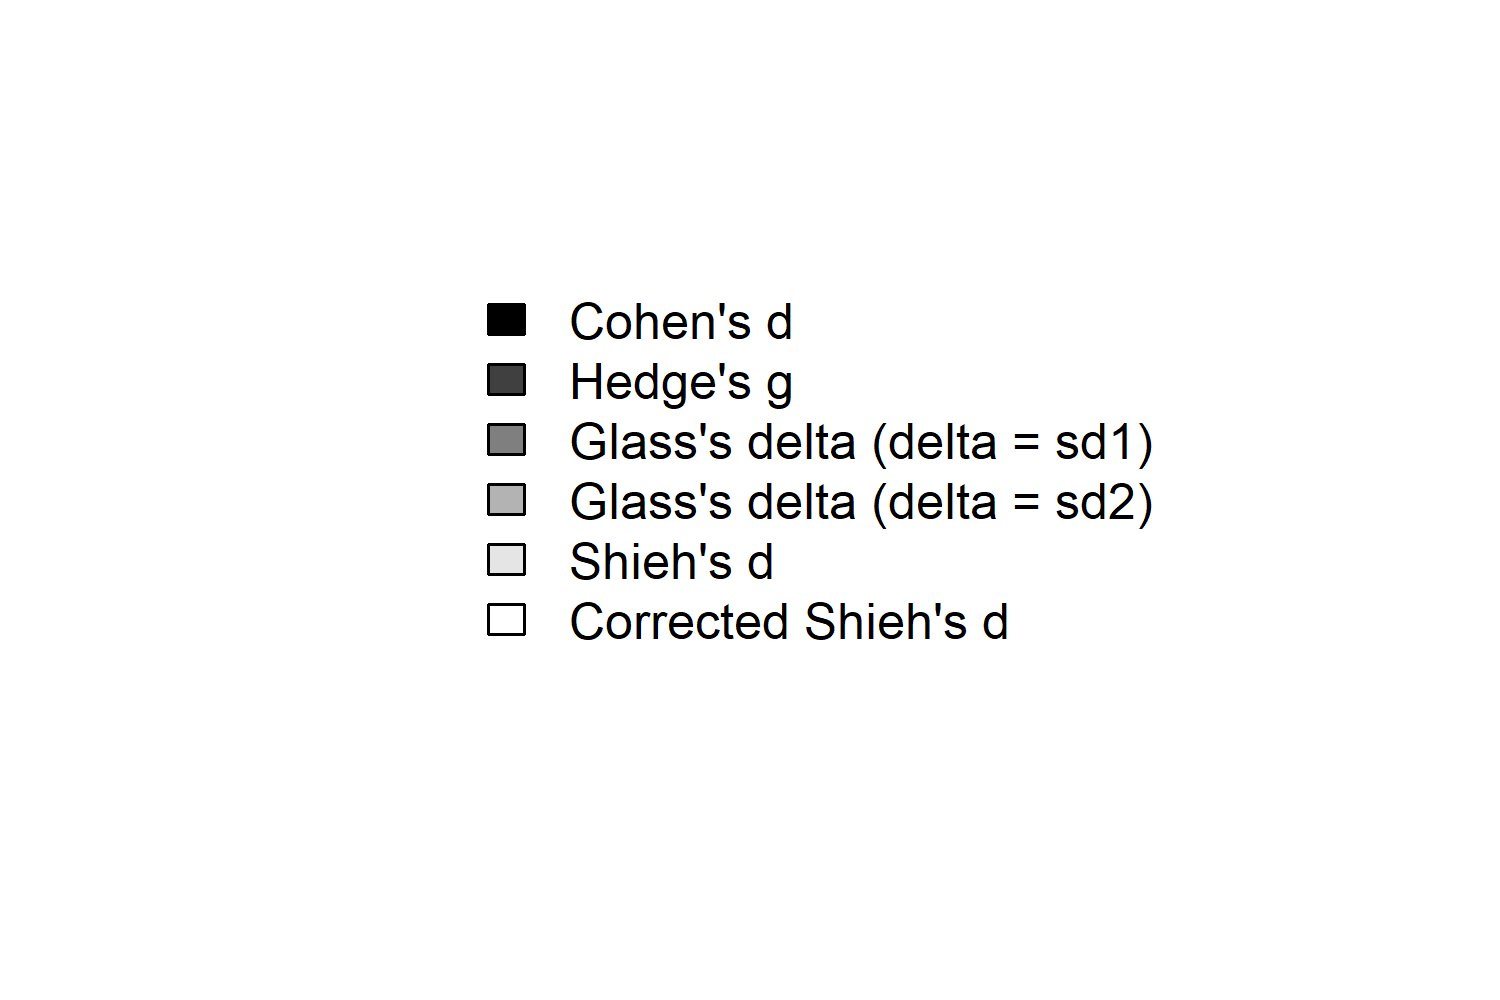
\includegraphics[width=400px]{C:/Users/Marie/Documents/Github_projects/Effect-sizes/Scripts outputs/Quality of ES measures/Graphs/legend} \caption{Legend}\label{fig:legend}
\end{figure}

Figures \ref{fig:idHombal} and \ref{fig:idHetbal} show that for all configurations where sample sizes are equal between groups (conditions a and c), estimator bias tends to decrease and precision is also improved with increasing sample sizes, meaning that all estimators are consistent. Moreover, Shieh's \(d_s\) and Shieh's \(d^*_s\) are identical, because our transformation is operant only when the sample sizes ratio differs from 1. We can demonstrate that the bias of Shieh's \(d_s\) and Shieh's \(d_s^*\) is exactly half the size of Cohen's \(d_s\), and that their variance is exactly four times smaller than Cohen's \(d_s\). Due to the relation described in equation \ref{eq:cohenshieh} when sample sizes are equal between groups, such proportions mean that relative to their respective true effect size, Cohen's \(d_s\), Shieh's \(d_s\) and Shieh's \(d^*_s\) perform all as well, as we can see in the second and fourth rows in Figures \ref{fig:idHombal} and \ref{fig:idHetbal}. These two rows also reveal that the relative bias and variance of Hedges's \(g_s\) is also identical to the three prementioned ones.

\begin{equation} 
Shieh's \; \delta_{n_1=n_2}= \frac{Cohen's \; \delta_{n_1=n_2}}{2}
\label{eq:cohenshieh}
\end{equation}

Glass's \(d_s\) does not behave identically, depending on whether population variances are equal across groups (Figure \ref{fig:idHombal}) or not (Figure \ref{fig:idHetbal}). In Figure \ref{fig:idHombal}, glass's \(d_s\) shows least precision and highest bias rates, in comparison with all other measures, which is not surprising, as the standardizer is estimated based on half the sample size. As long as distributions are symmetric, both glass's \(d_s\) estimates (i.e.~using \(SD_1\) and \(SD_2\)) show similar performances. However, it does not hold when distributions are skewed because of a non null correlation between the sample mean and standard deviation (resulting in a non null correlation between \(\bar{X_1}-\bar{X_2}\) and respectively \(SD_1\) and \(SD_2\)). Because the population mean difference is positive in all our simulations (i.e.~\(\mu_1-\mu_2>0\)), Glass's \(d_s\) is always more biased and variable when choosing as standardizer the SD that is negatively correlated with \(\bar{X_1}-\bar{X_2}\) (i.e.~\(SD_2\) when distributions are right-skewed and \(SD_1\) when distributions are left-skewed; for interested reader, see the Appendix 3). \footnote{When the population mean difference is negative (i.e. $\mu_1-\mu_2<0$), Glass's $d_s$ will always be more biased and variable when choosing as standardizer the SD that is positively correlated with $\bar{X_1}-\bar{X_2}$ (i.e. $SD_1$ when distributions are right-skewed and $SD_2$ when distributions are left-skewed).}

In Figure \ref{fig:idHetbal} \ldots{} (décrire le glass dans ce cas). As previously, both glass's \(d_s\) estimates (i.e.~using \(SD_1\) and \(SD_2\)) show similar bias rate when distribution are symmetric.\footnote{When looking at Figure 4, one could believe that the bias is always more important when choosing SD2 as a standardizer. It is only an artefact of simulations. The bias is always more important when choosing the sample extracted from the smaller population SD as standardiser, because it results in a larger effect size estimate, and the larger the effect size estimate, the larger the raw bias. In our simulations, while the population SD of the first group always equals 1, in half of the simulations in condition c, the population SD of the second group is lower than 1 (meaning that the more biased Glass's estimate will occure when choosing SD2 < 1 as standardiser), and in the other half, the population SD of the second group is larger than 1 (meaning that the more biased Glass's estimate will occure when choosing SD1 as standardizer). Of course, for X, a constant mean difference and z, the standardizer, X/z will always result in a larger effect size measure when z < 1. This is confirmed by the identical average relative bias for both measures of Glass's ds.}. However, when distributions are skewed\ldots LA, PARFOIS GLASS EST LE MEILLEUR, PARFOIS C EST LE PIRE. ETUDIER CA EN DETAIL.

Rem: par contre, se passe un truc au niveau de la variance relative quand distribution heavy-tailed: étudier ça!

\begin{sidewaysfigure}

{\centering 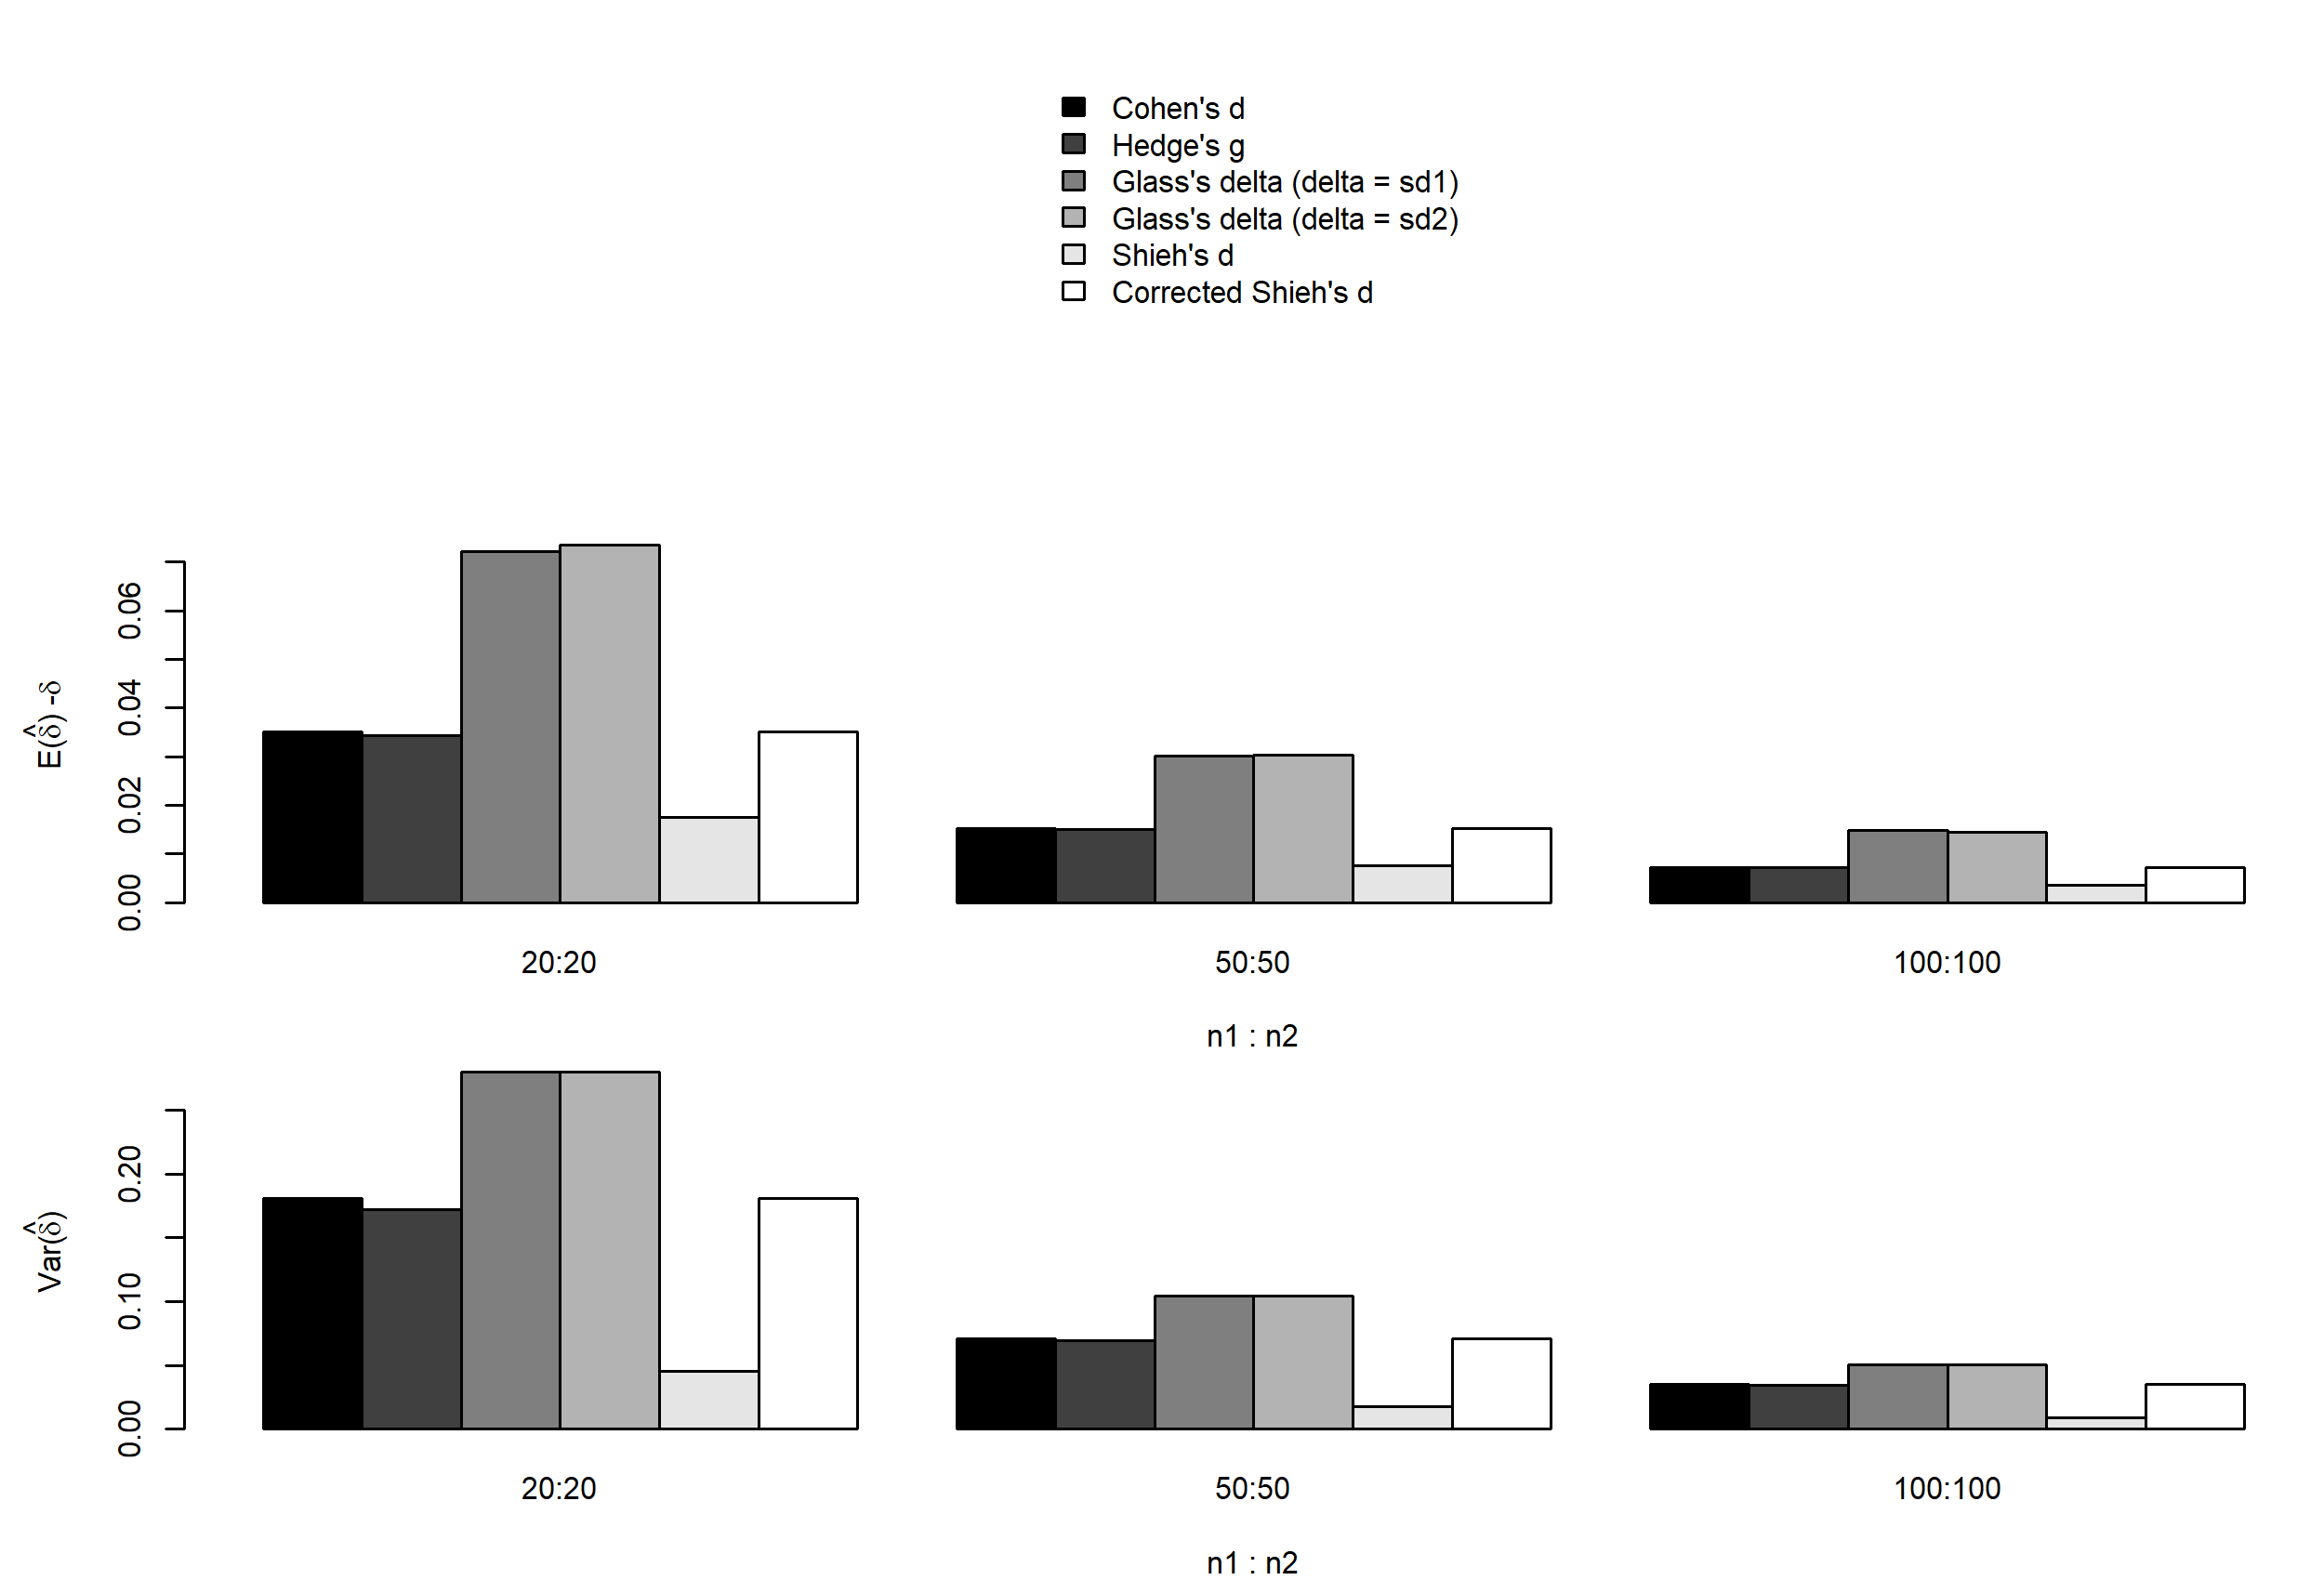
\includegraphics[width=0.2\linewidth]{C:/Users/Marie/Documents/Github_projects/Effect-sizes/Scripts outputs/Quality of ES measures/Graphs/id_Hom_bal/bias_eff,G1=0 & G2=0;id_Hom_bal} 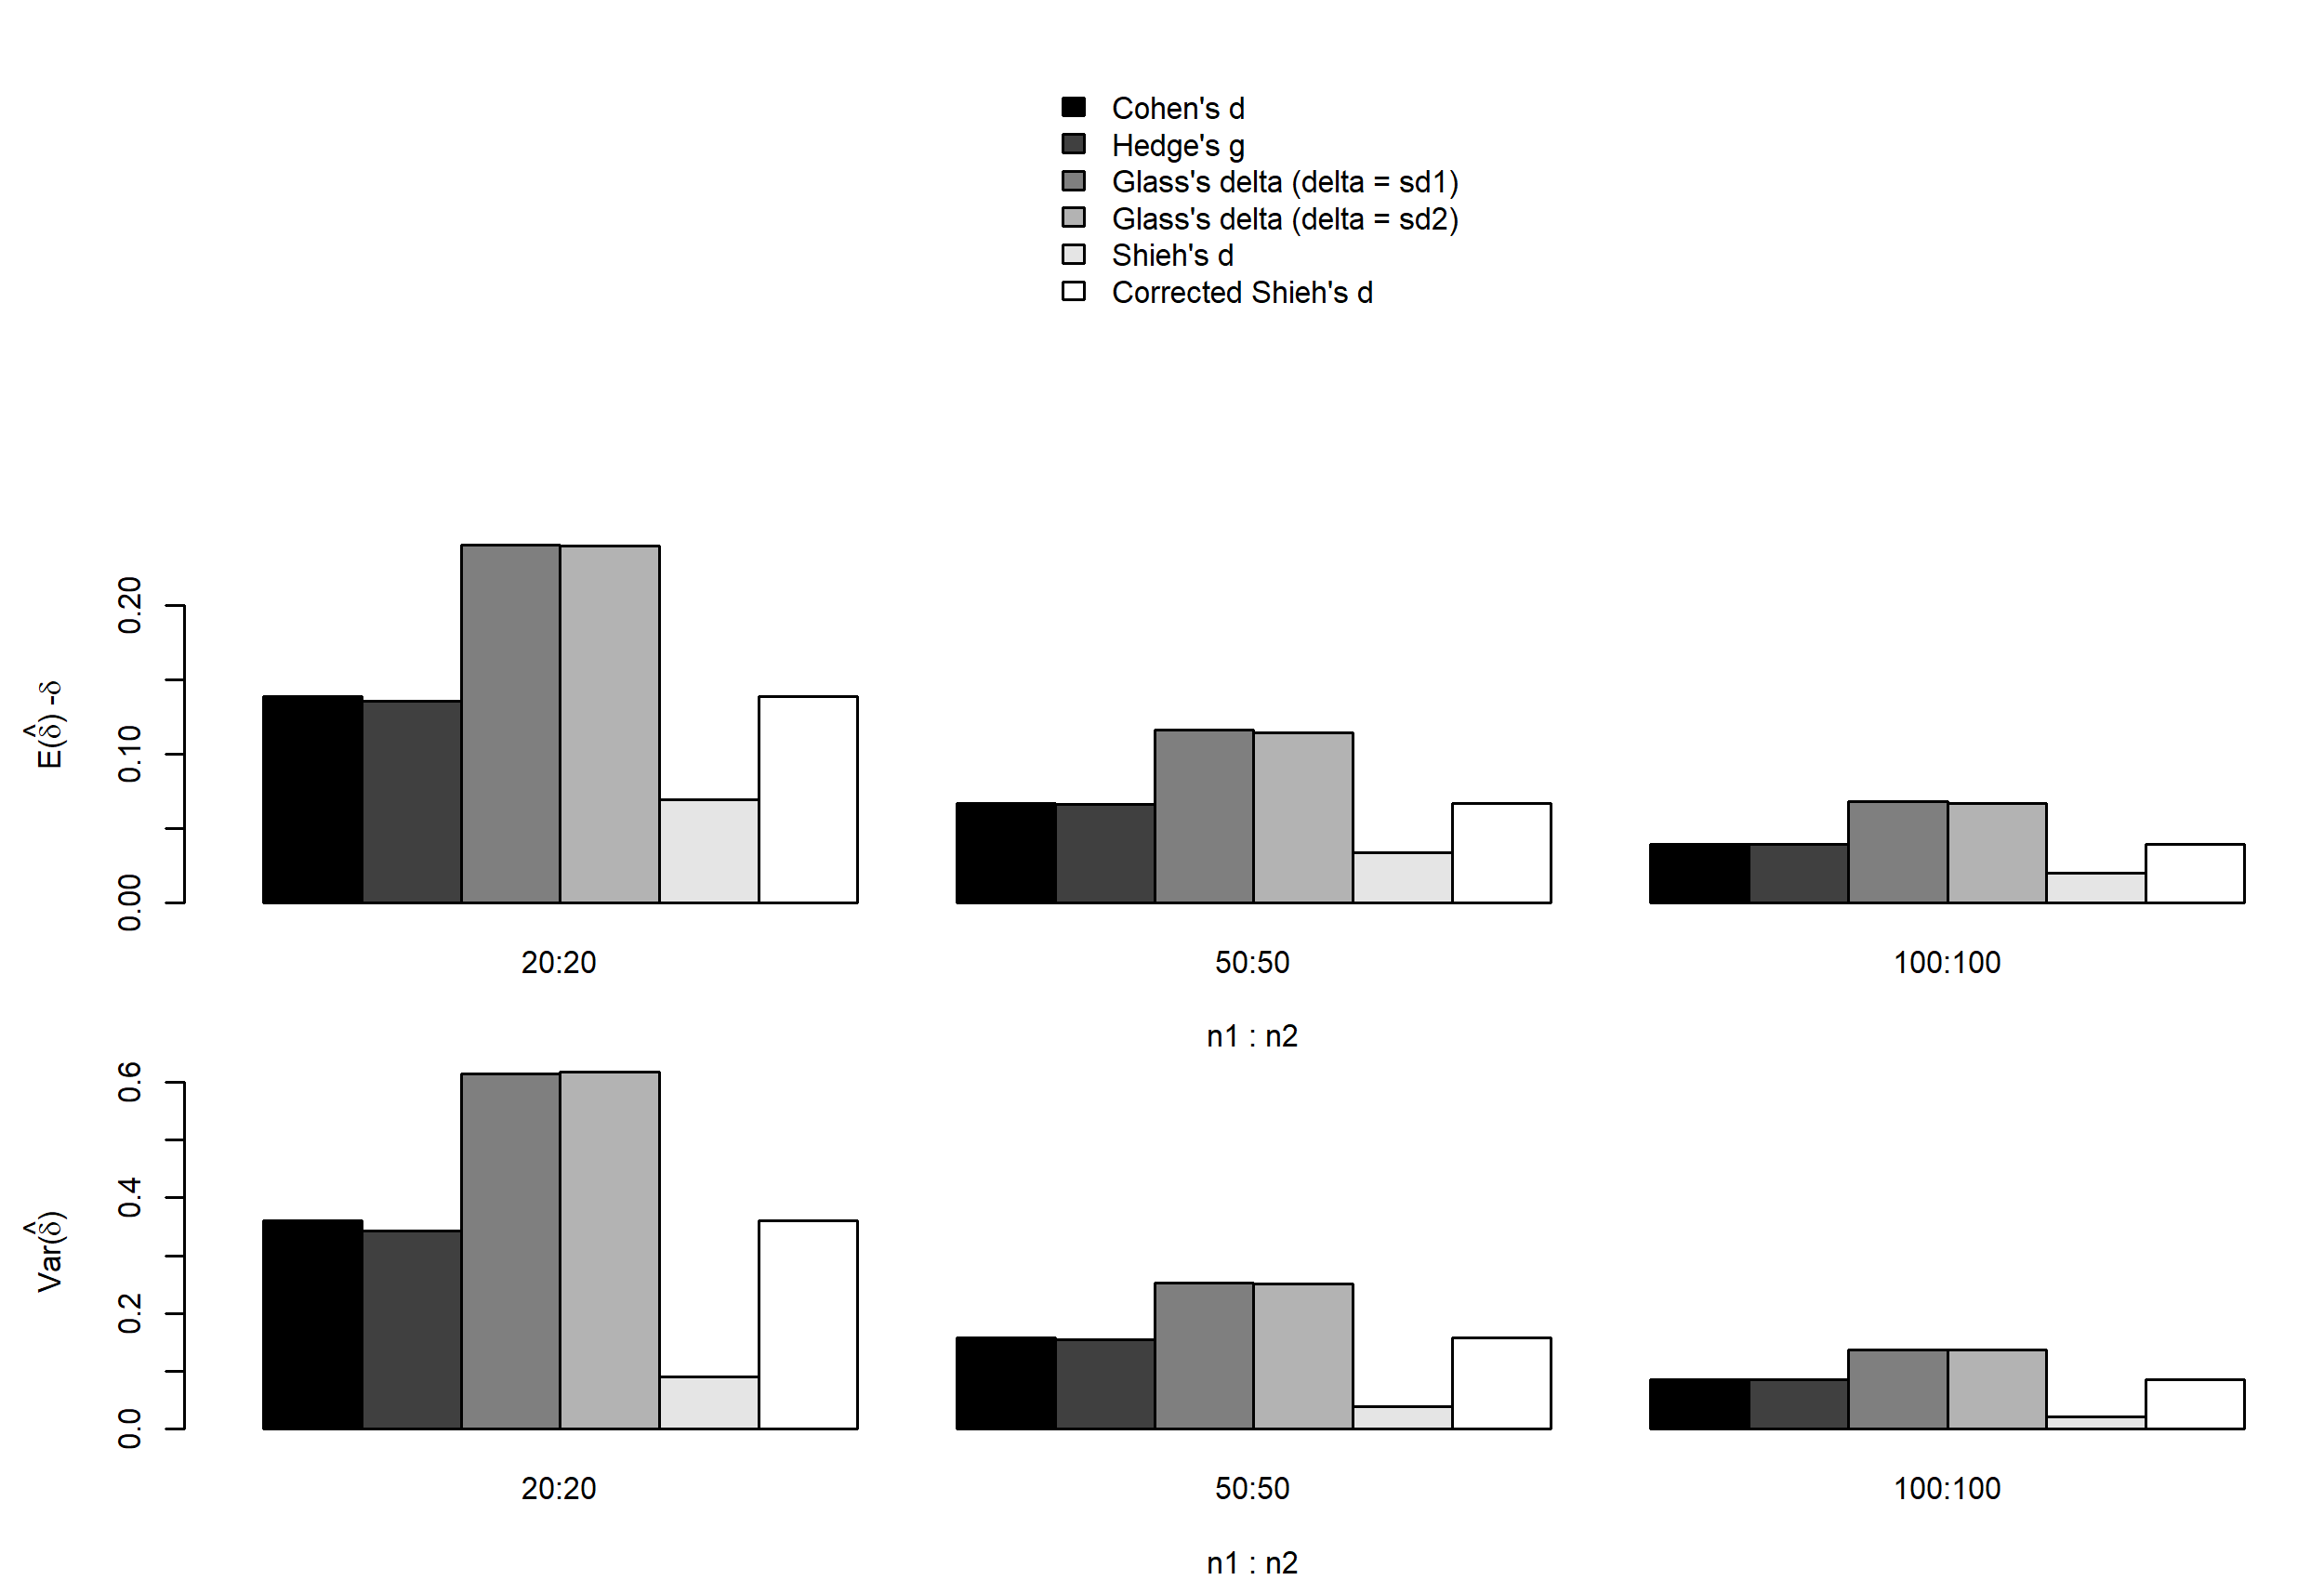
\includegraphics[width=0.2\linewidth]{C:/Users/Marie/Documents/Github_projects/Effect-sizes/Scripts outputs/Quality of ES measures/Graphs/id_Hom_bal/bias_eff,G1=0 & G2=95.75;id_Hom_bal} 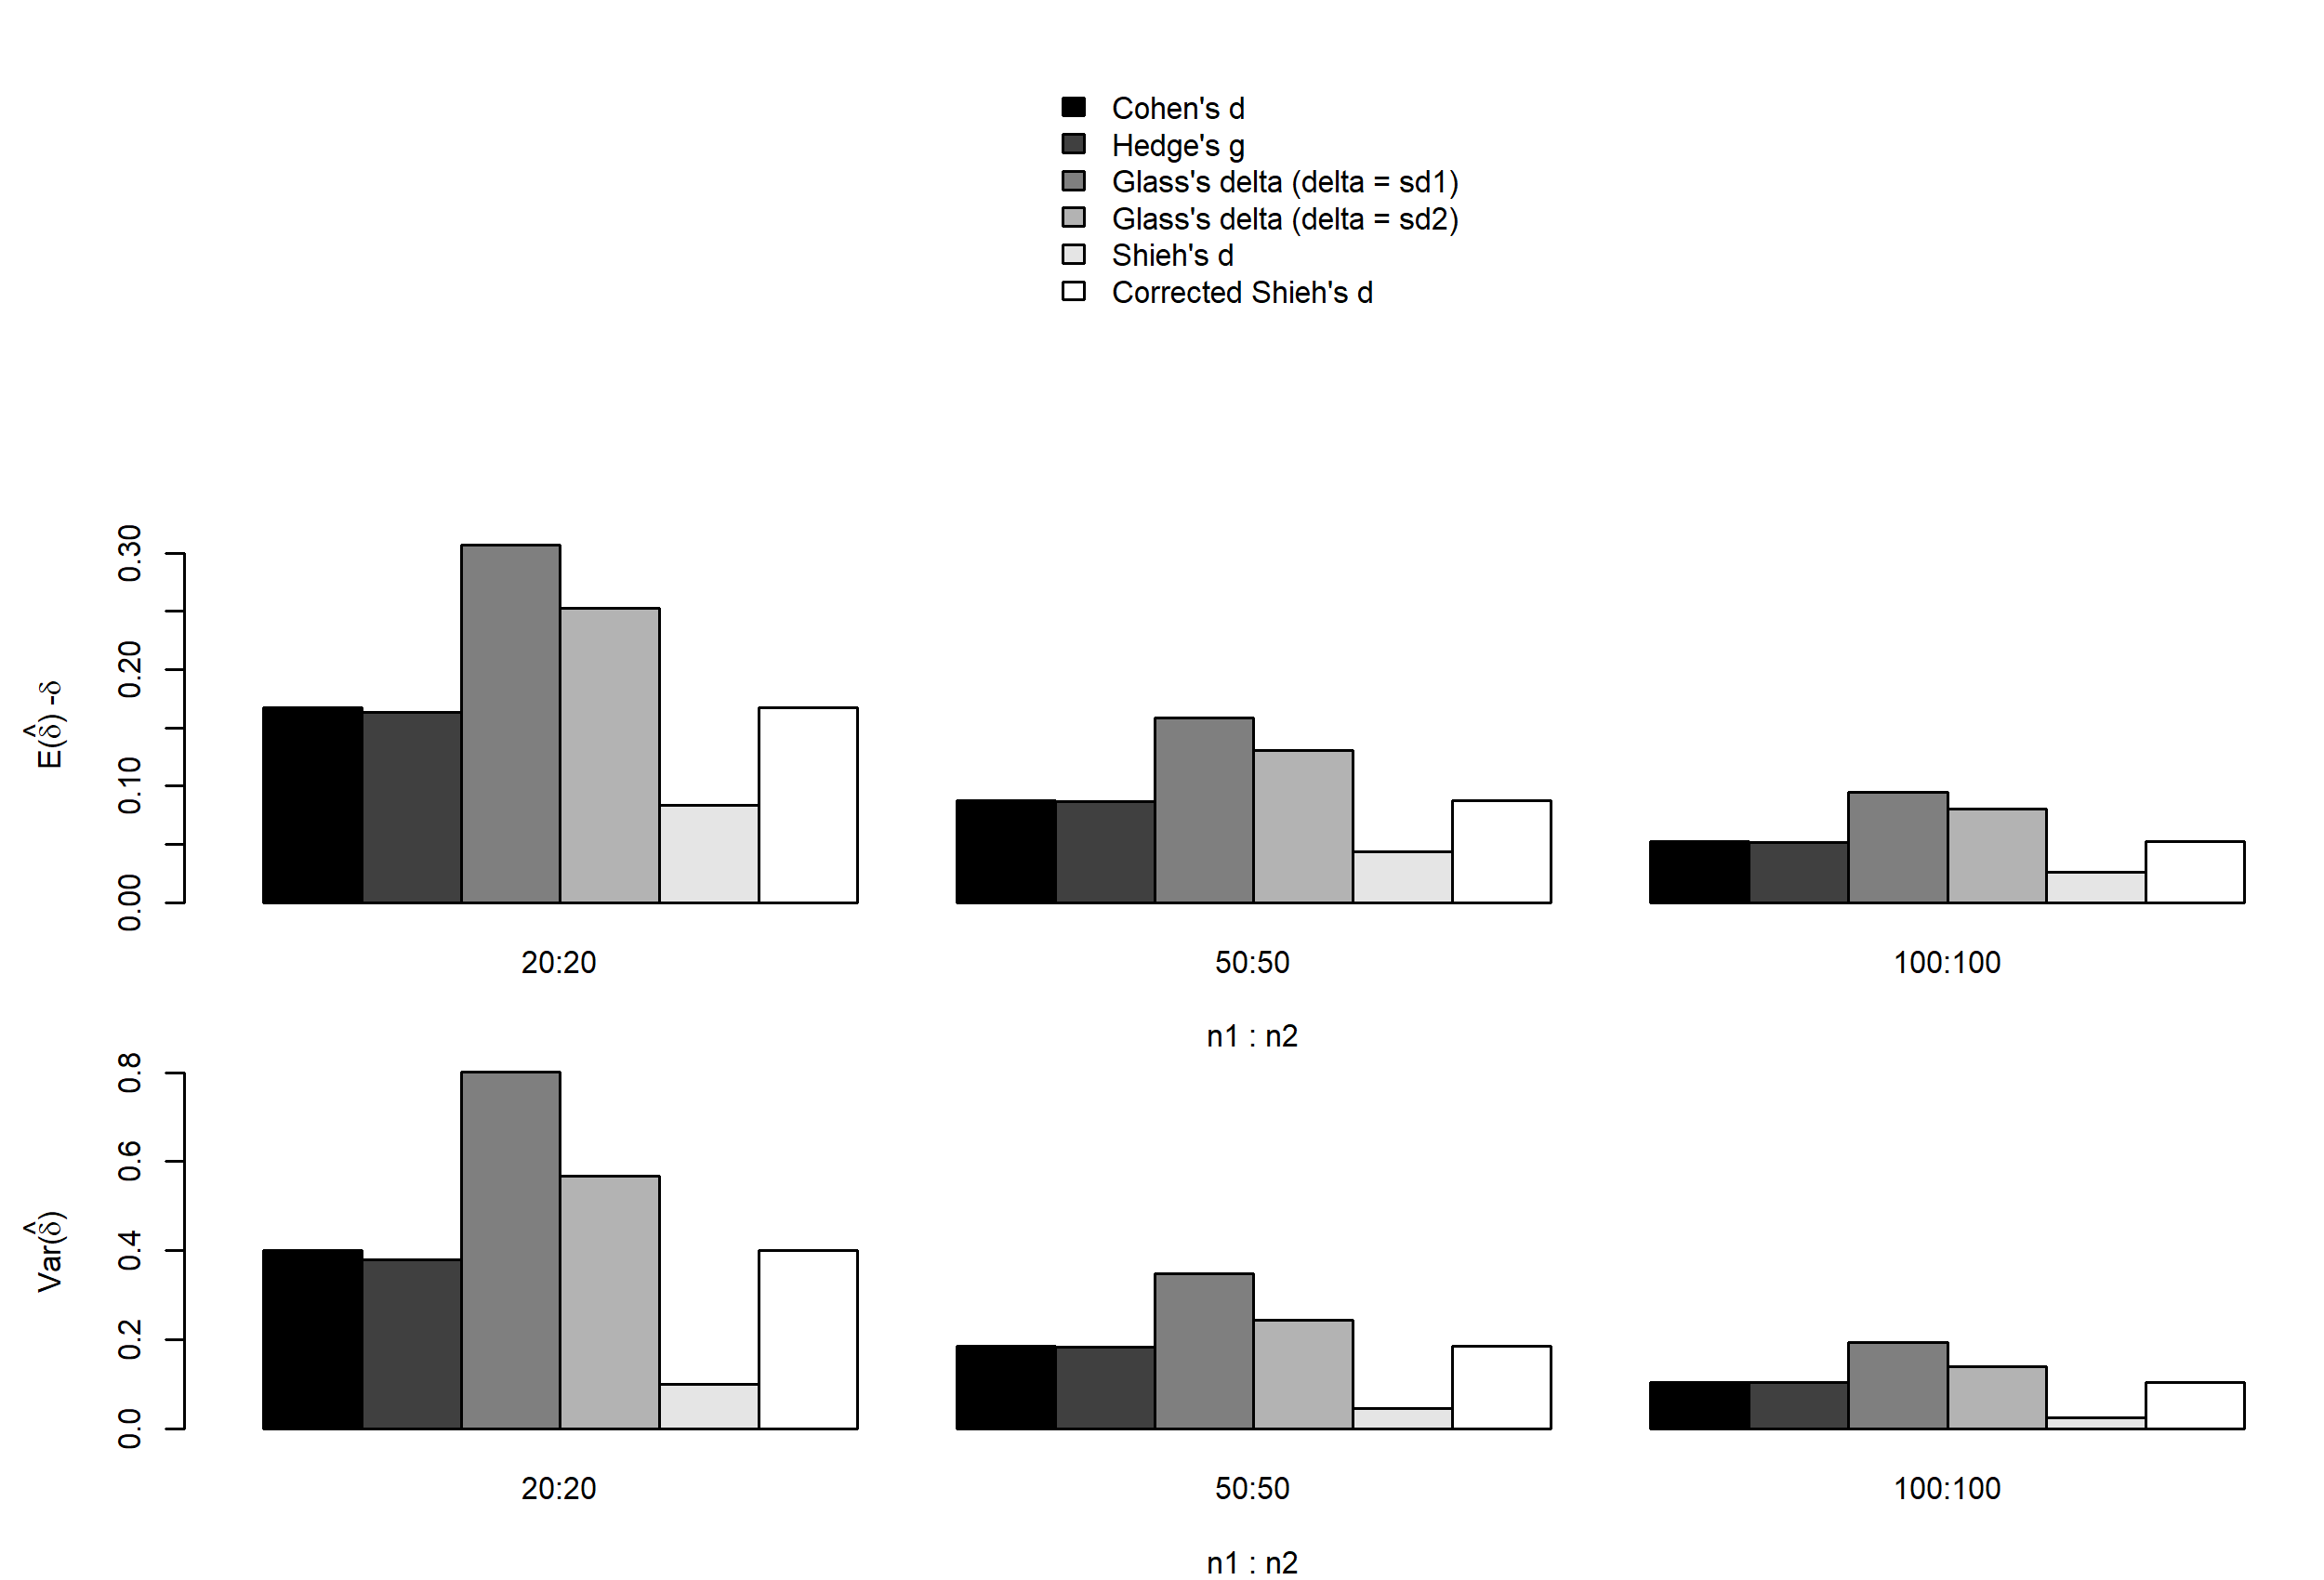
\includegraphics[width=0.2\linewidth]{C:/Users/Marie/Documents/Github_projects/Effect-sizes/Scripts outputs/Quality of ES measures/Graphs/id_Hom_bal/bias_eff,G1=2.08 & G2=95.75;id_Hom_bal} 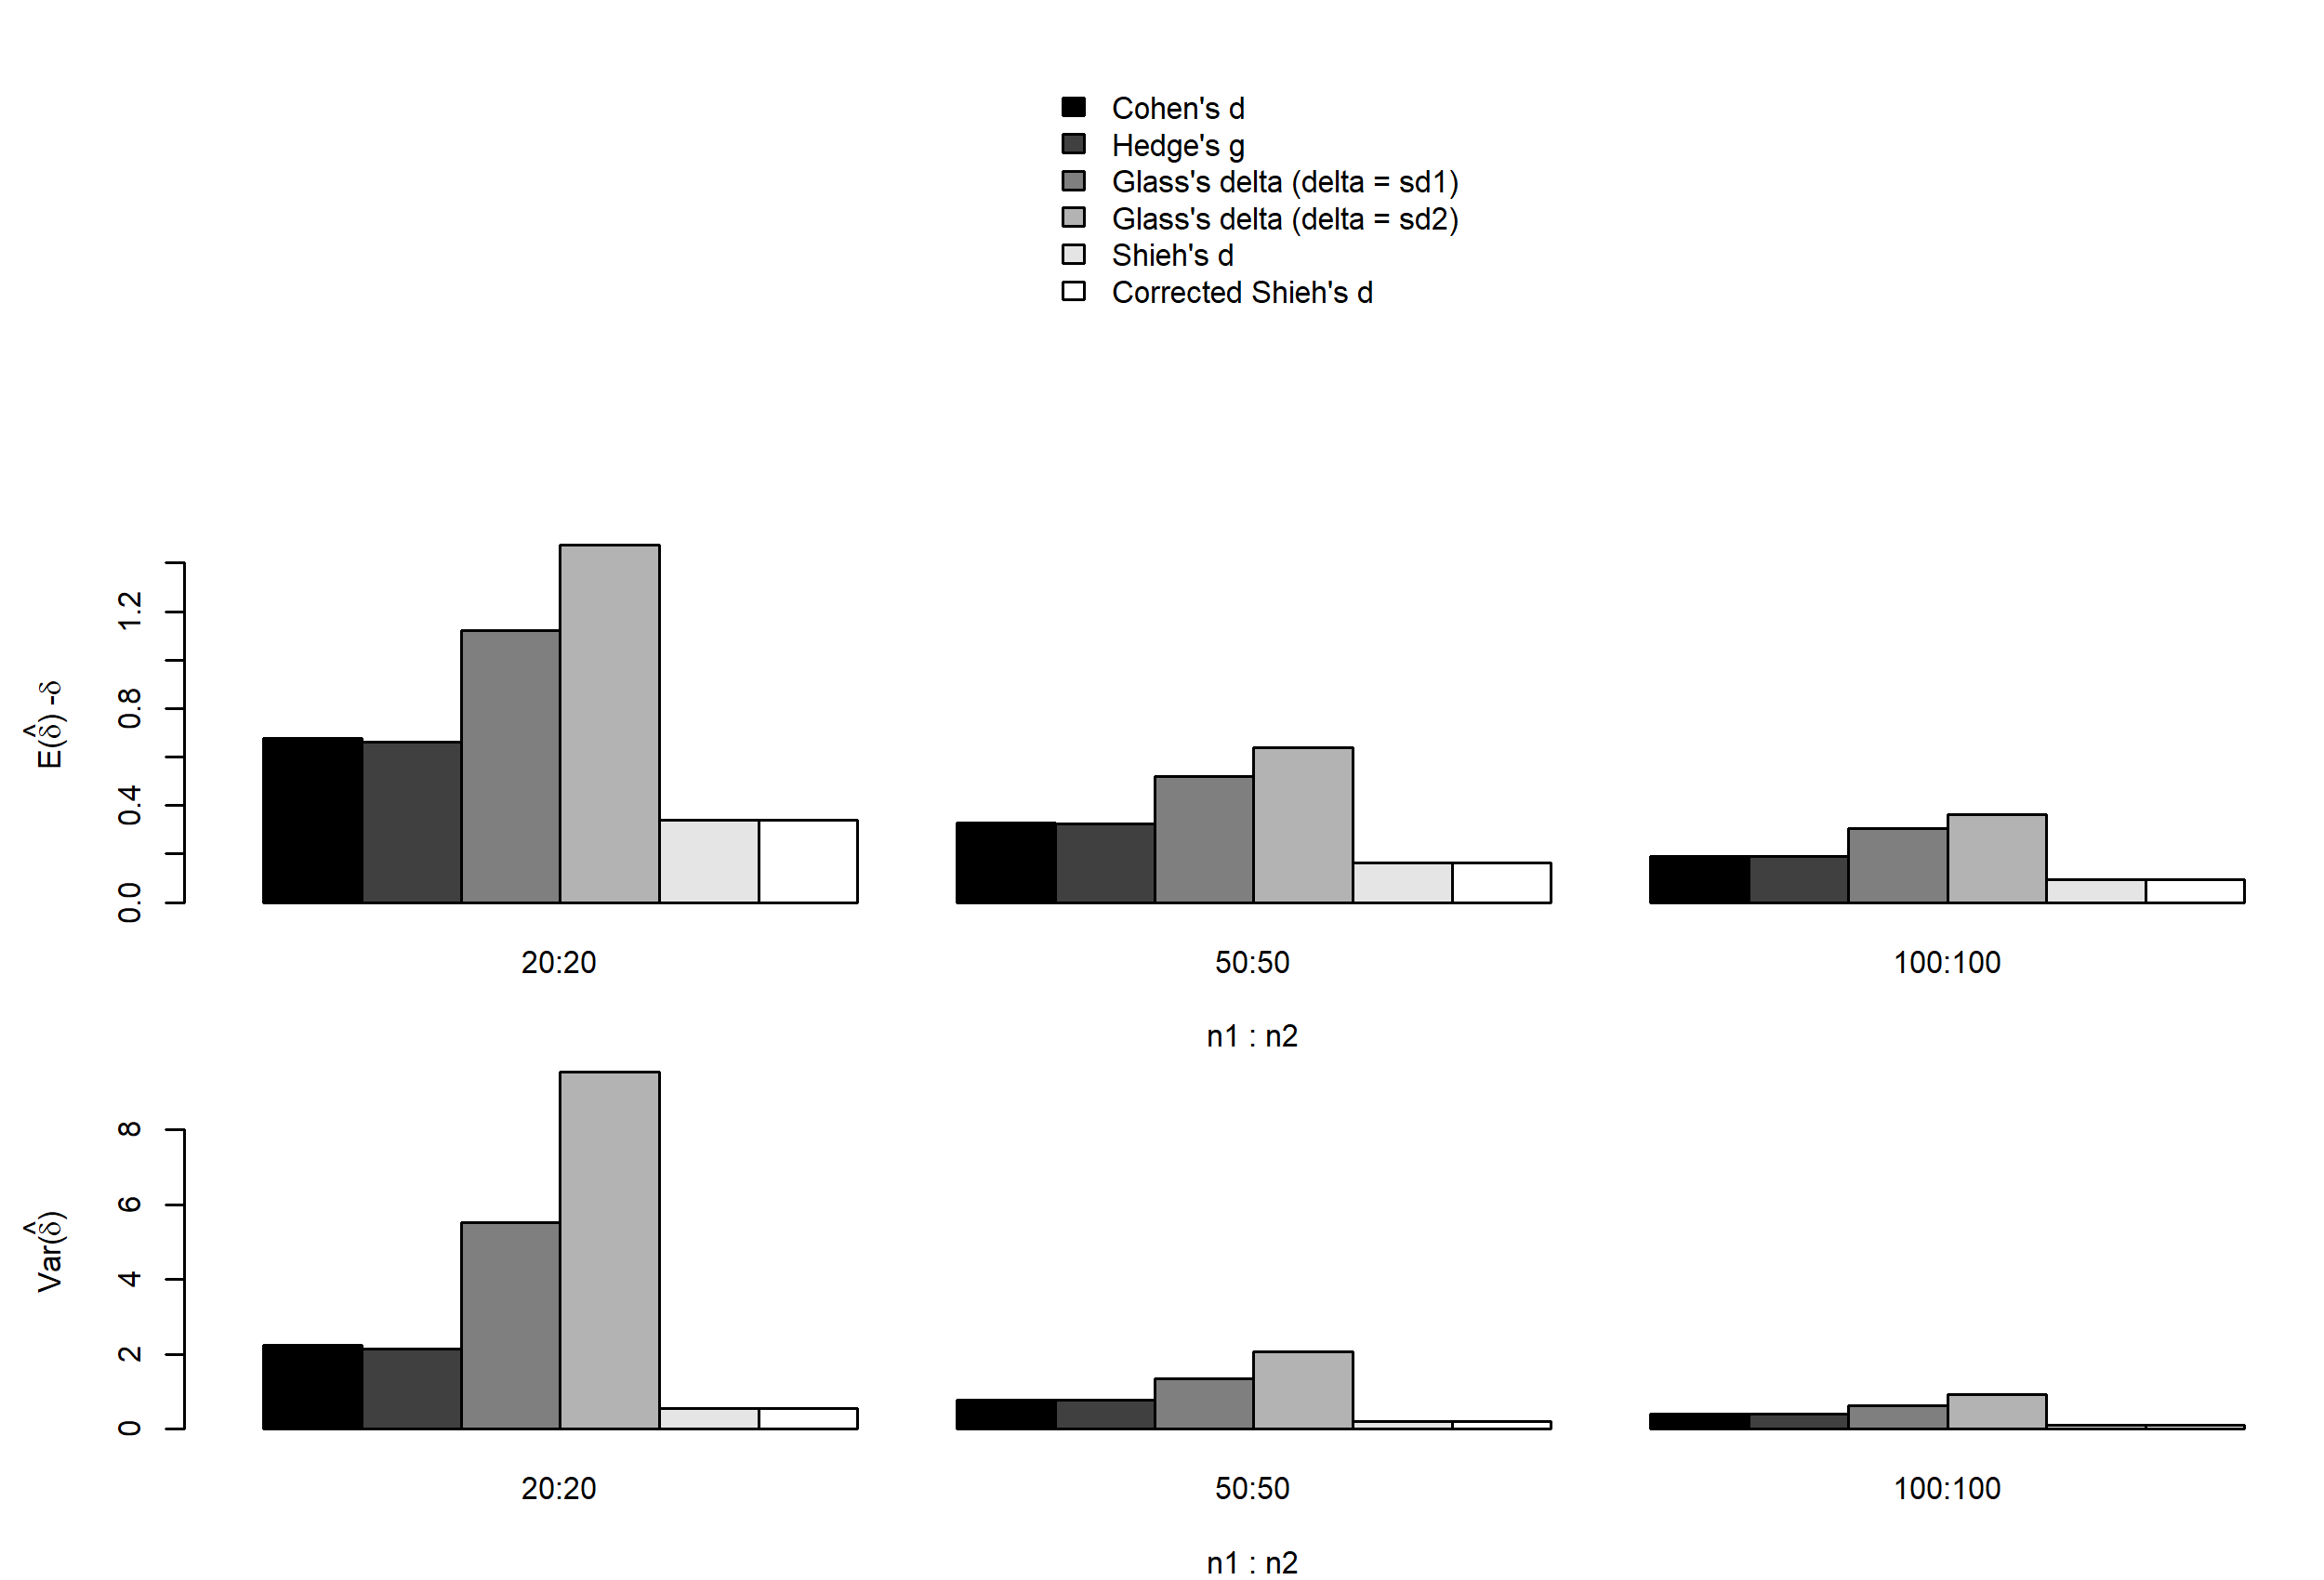
\includegraphics[width=0.2\linewidth]{C:/Users/Marie/Documents/Github_projects/Effect-sizes/Scripts outputs/Quality of ES measures/Graphs/id_Hom_bal/bias_eff,G1=6.32 & G2=95.75;id_Hom_bal} 

}

\caption{Bias and efficiency of five estimator of standardized mean difference, when variances and sample sizes are equal across groups (condition a)}\label{fig:idHombal}
\end{sidewaysfigure}

\begin{sidewaysfigure}

{\centering 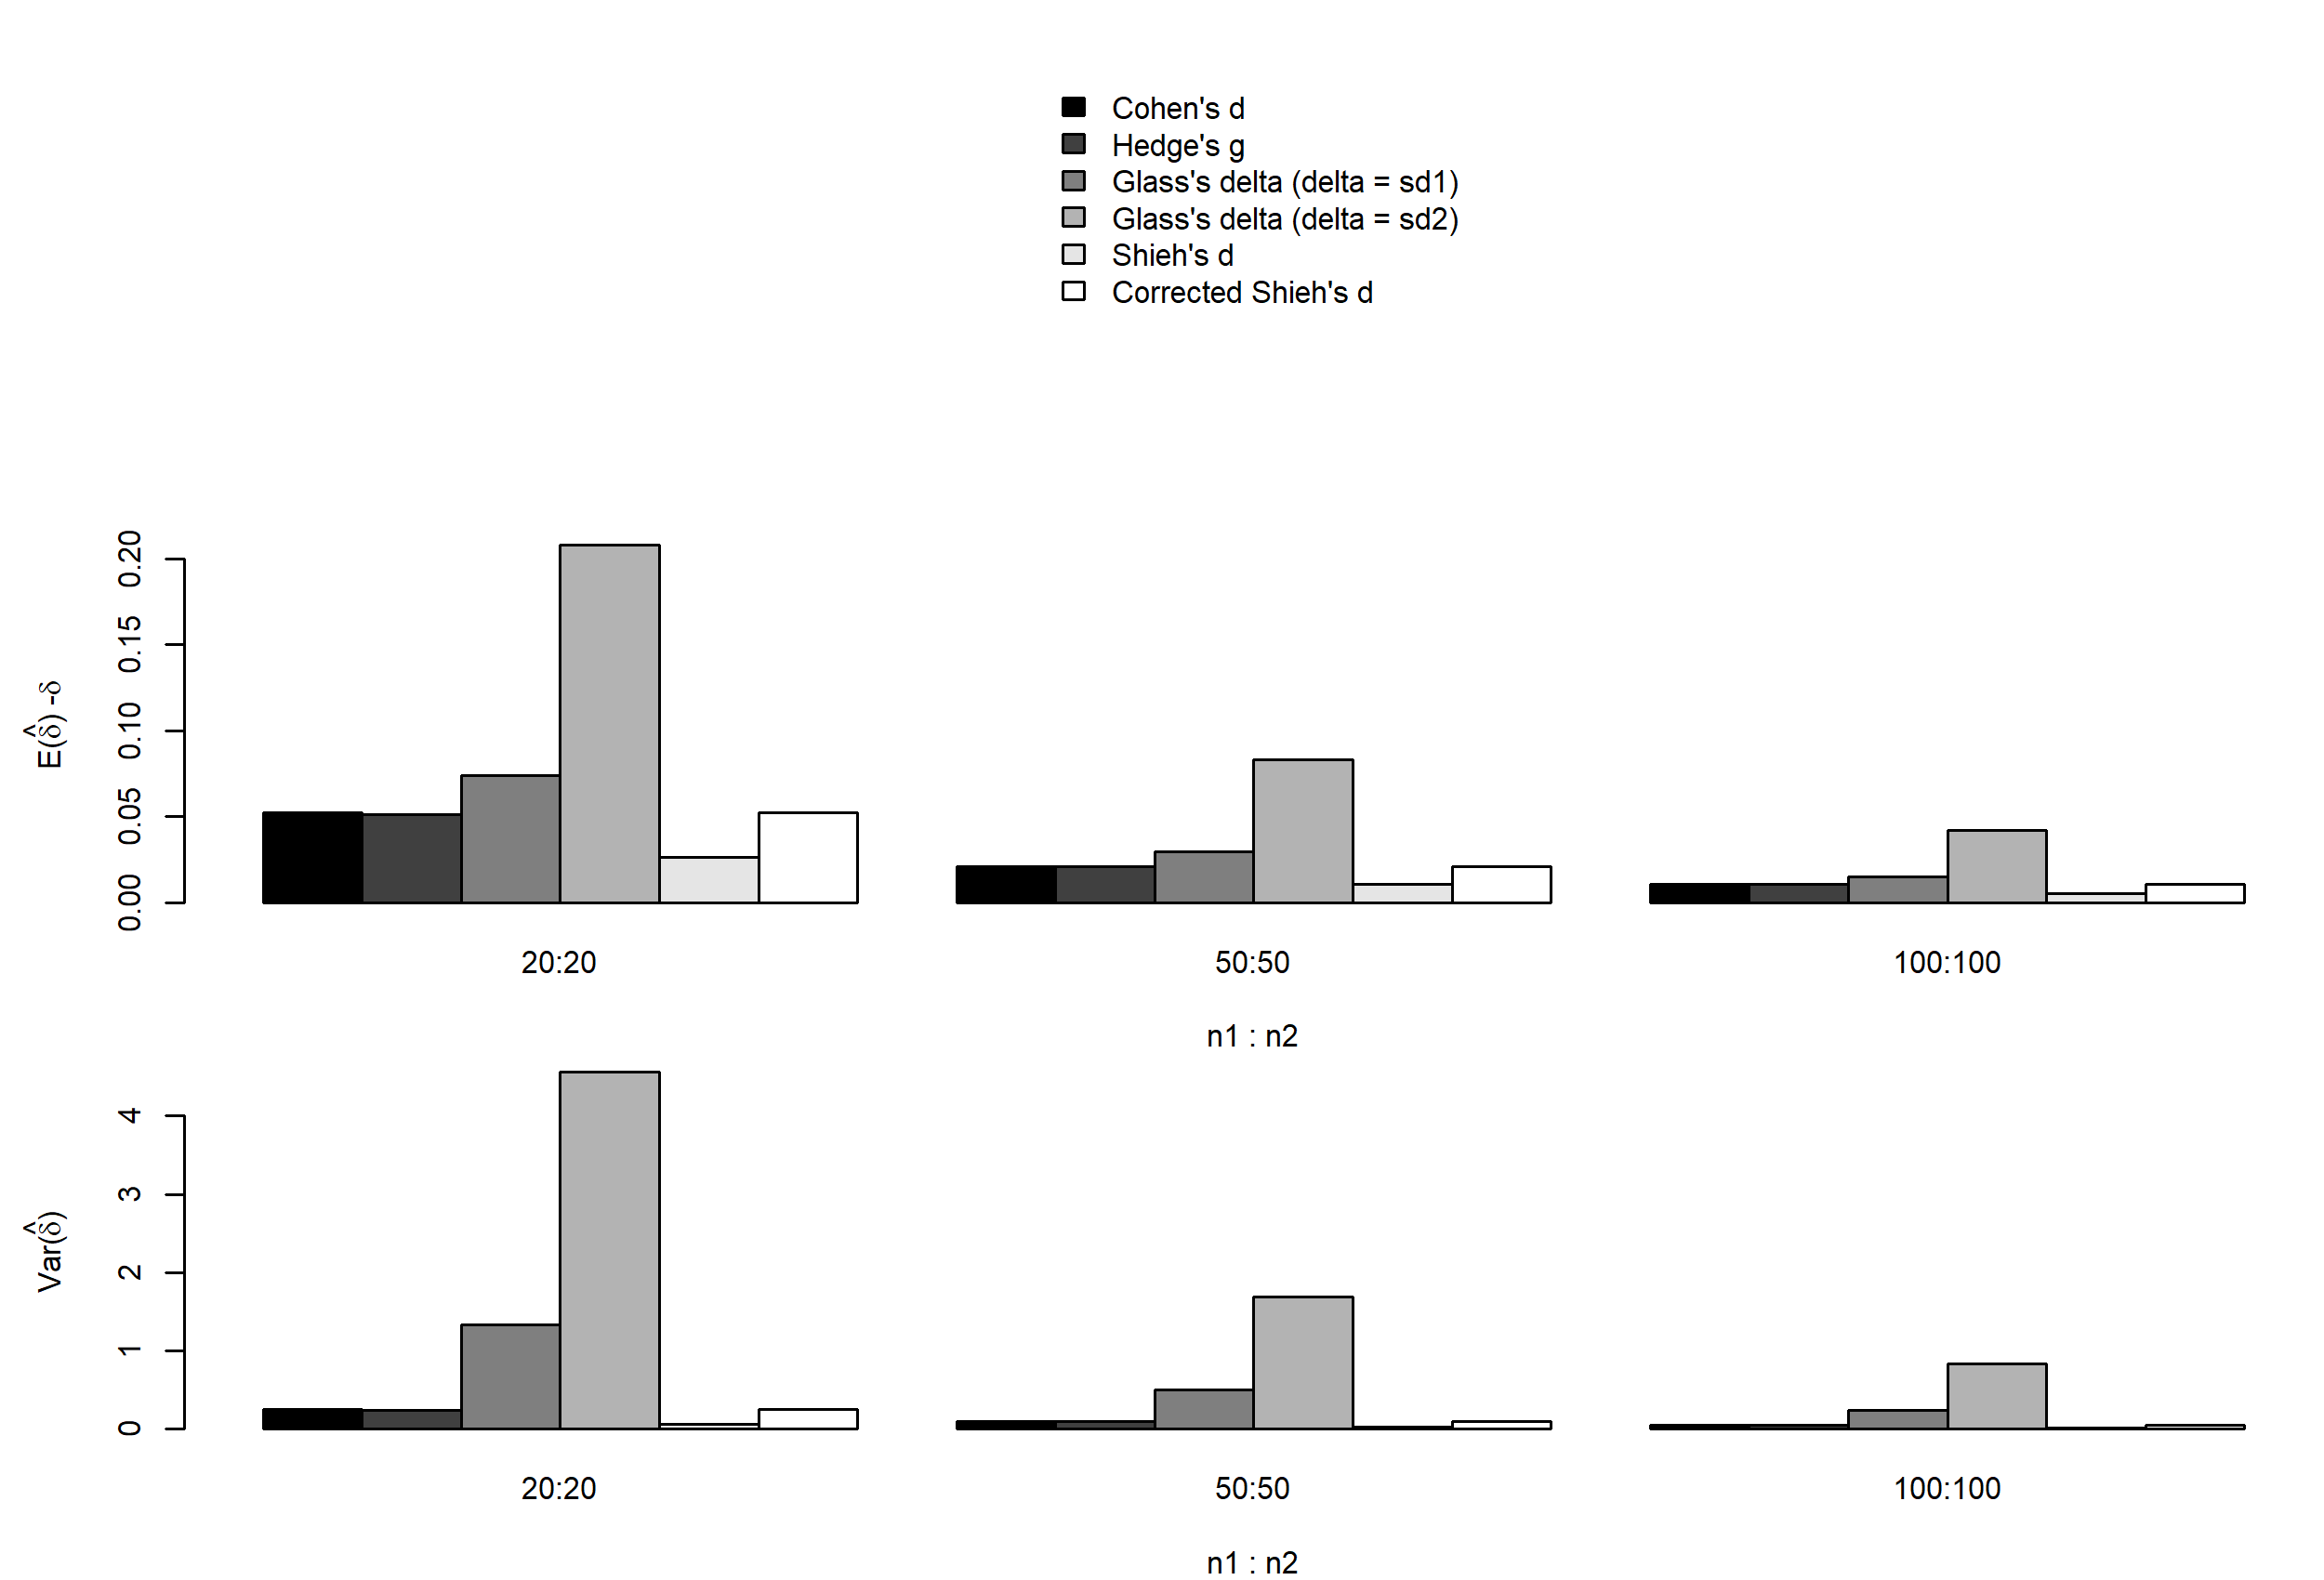
\includegraphics[width=0.2\linewidth]{C:/Users/Marie/Documents/Github_projects/Effect-sizes/Scripts outputs/Quality of ES measures/Graphs/id_Het_bal/bias_eff,G1=0 & G2=0;id_Het_bal} 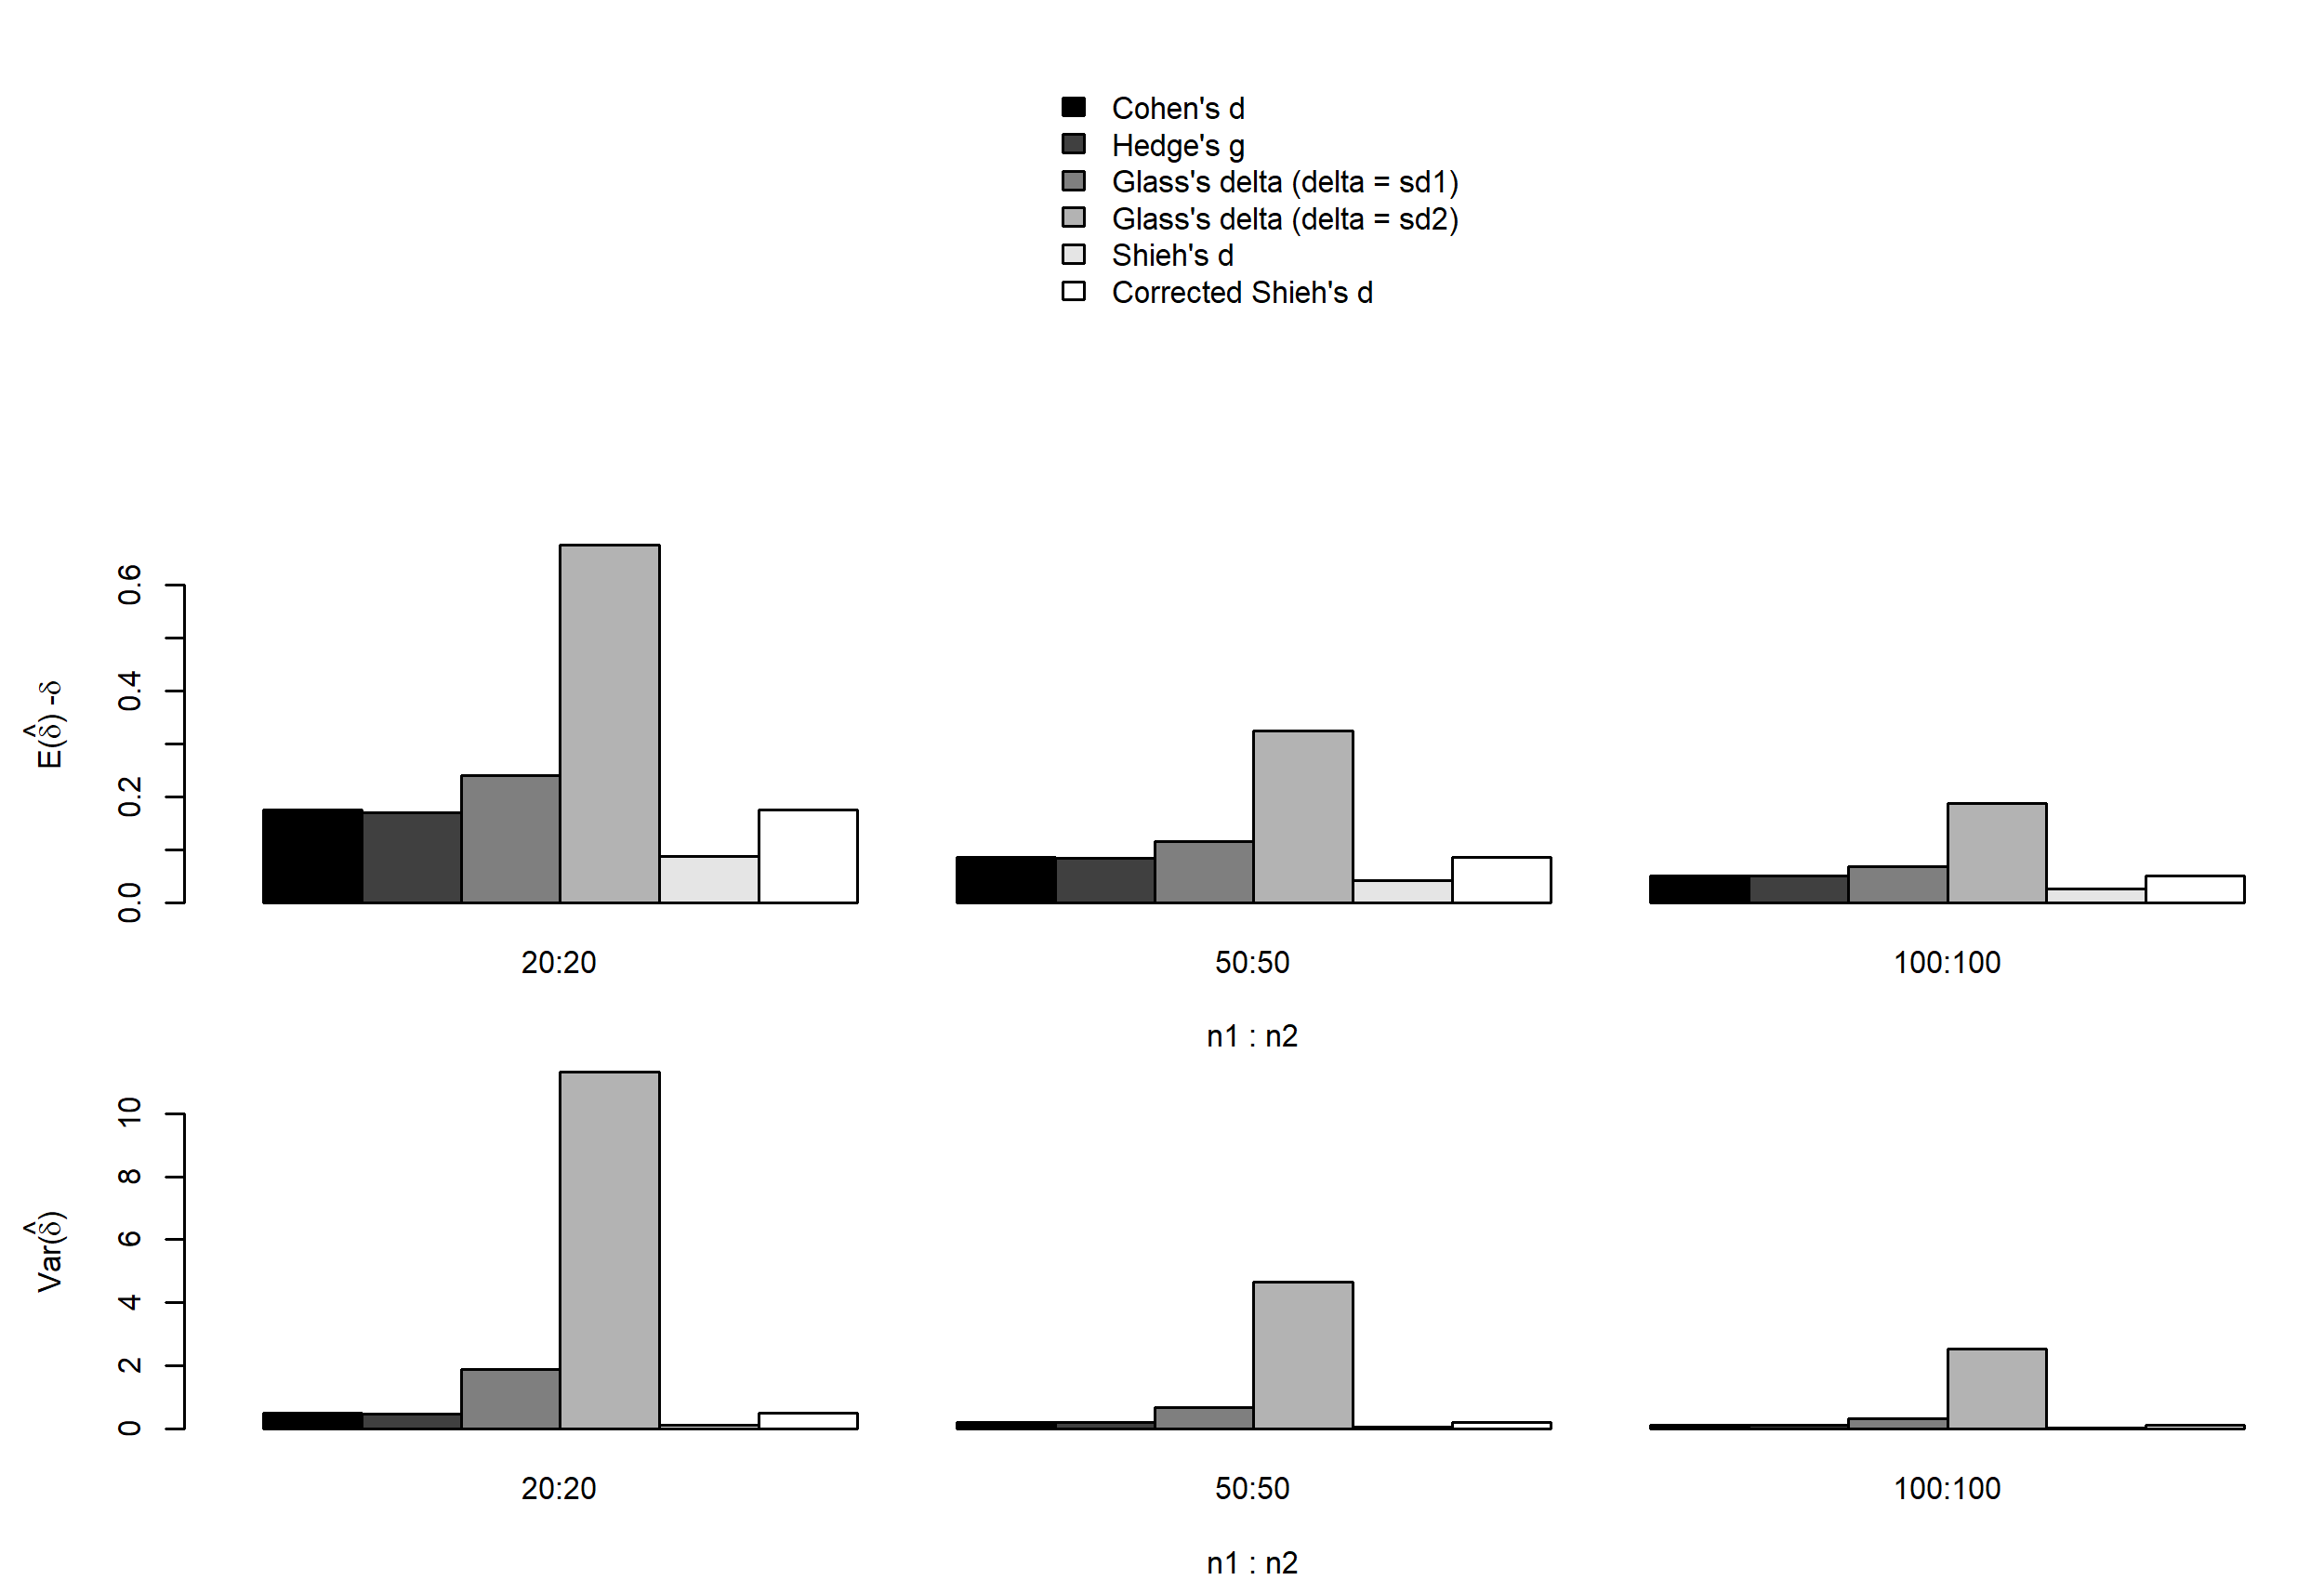
\includegraphics[width=0.2\linewidth]{C:/Users/Marie/Documents/Github_projects/Effect-sizes/Scripts outputs/Quality of ES measures/Graphs/id_Het_bal/bias_eff,G1=0 & G2=95.75;id_Het_bal} 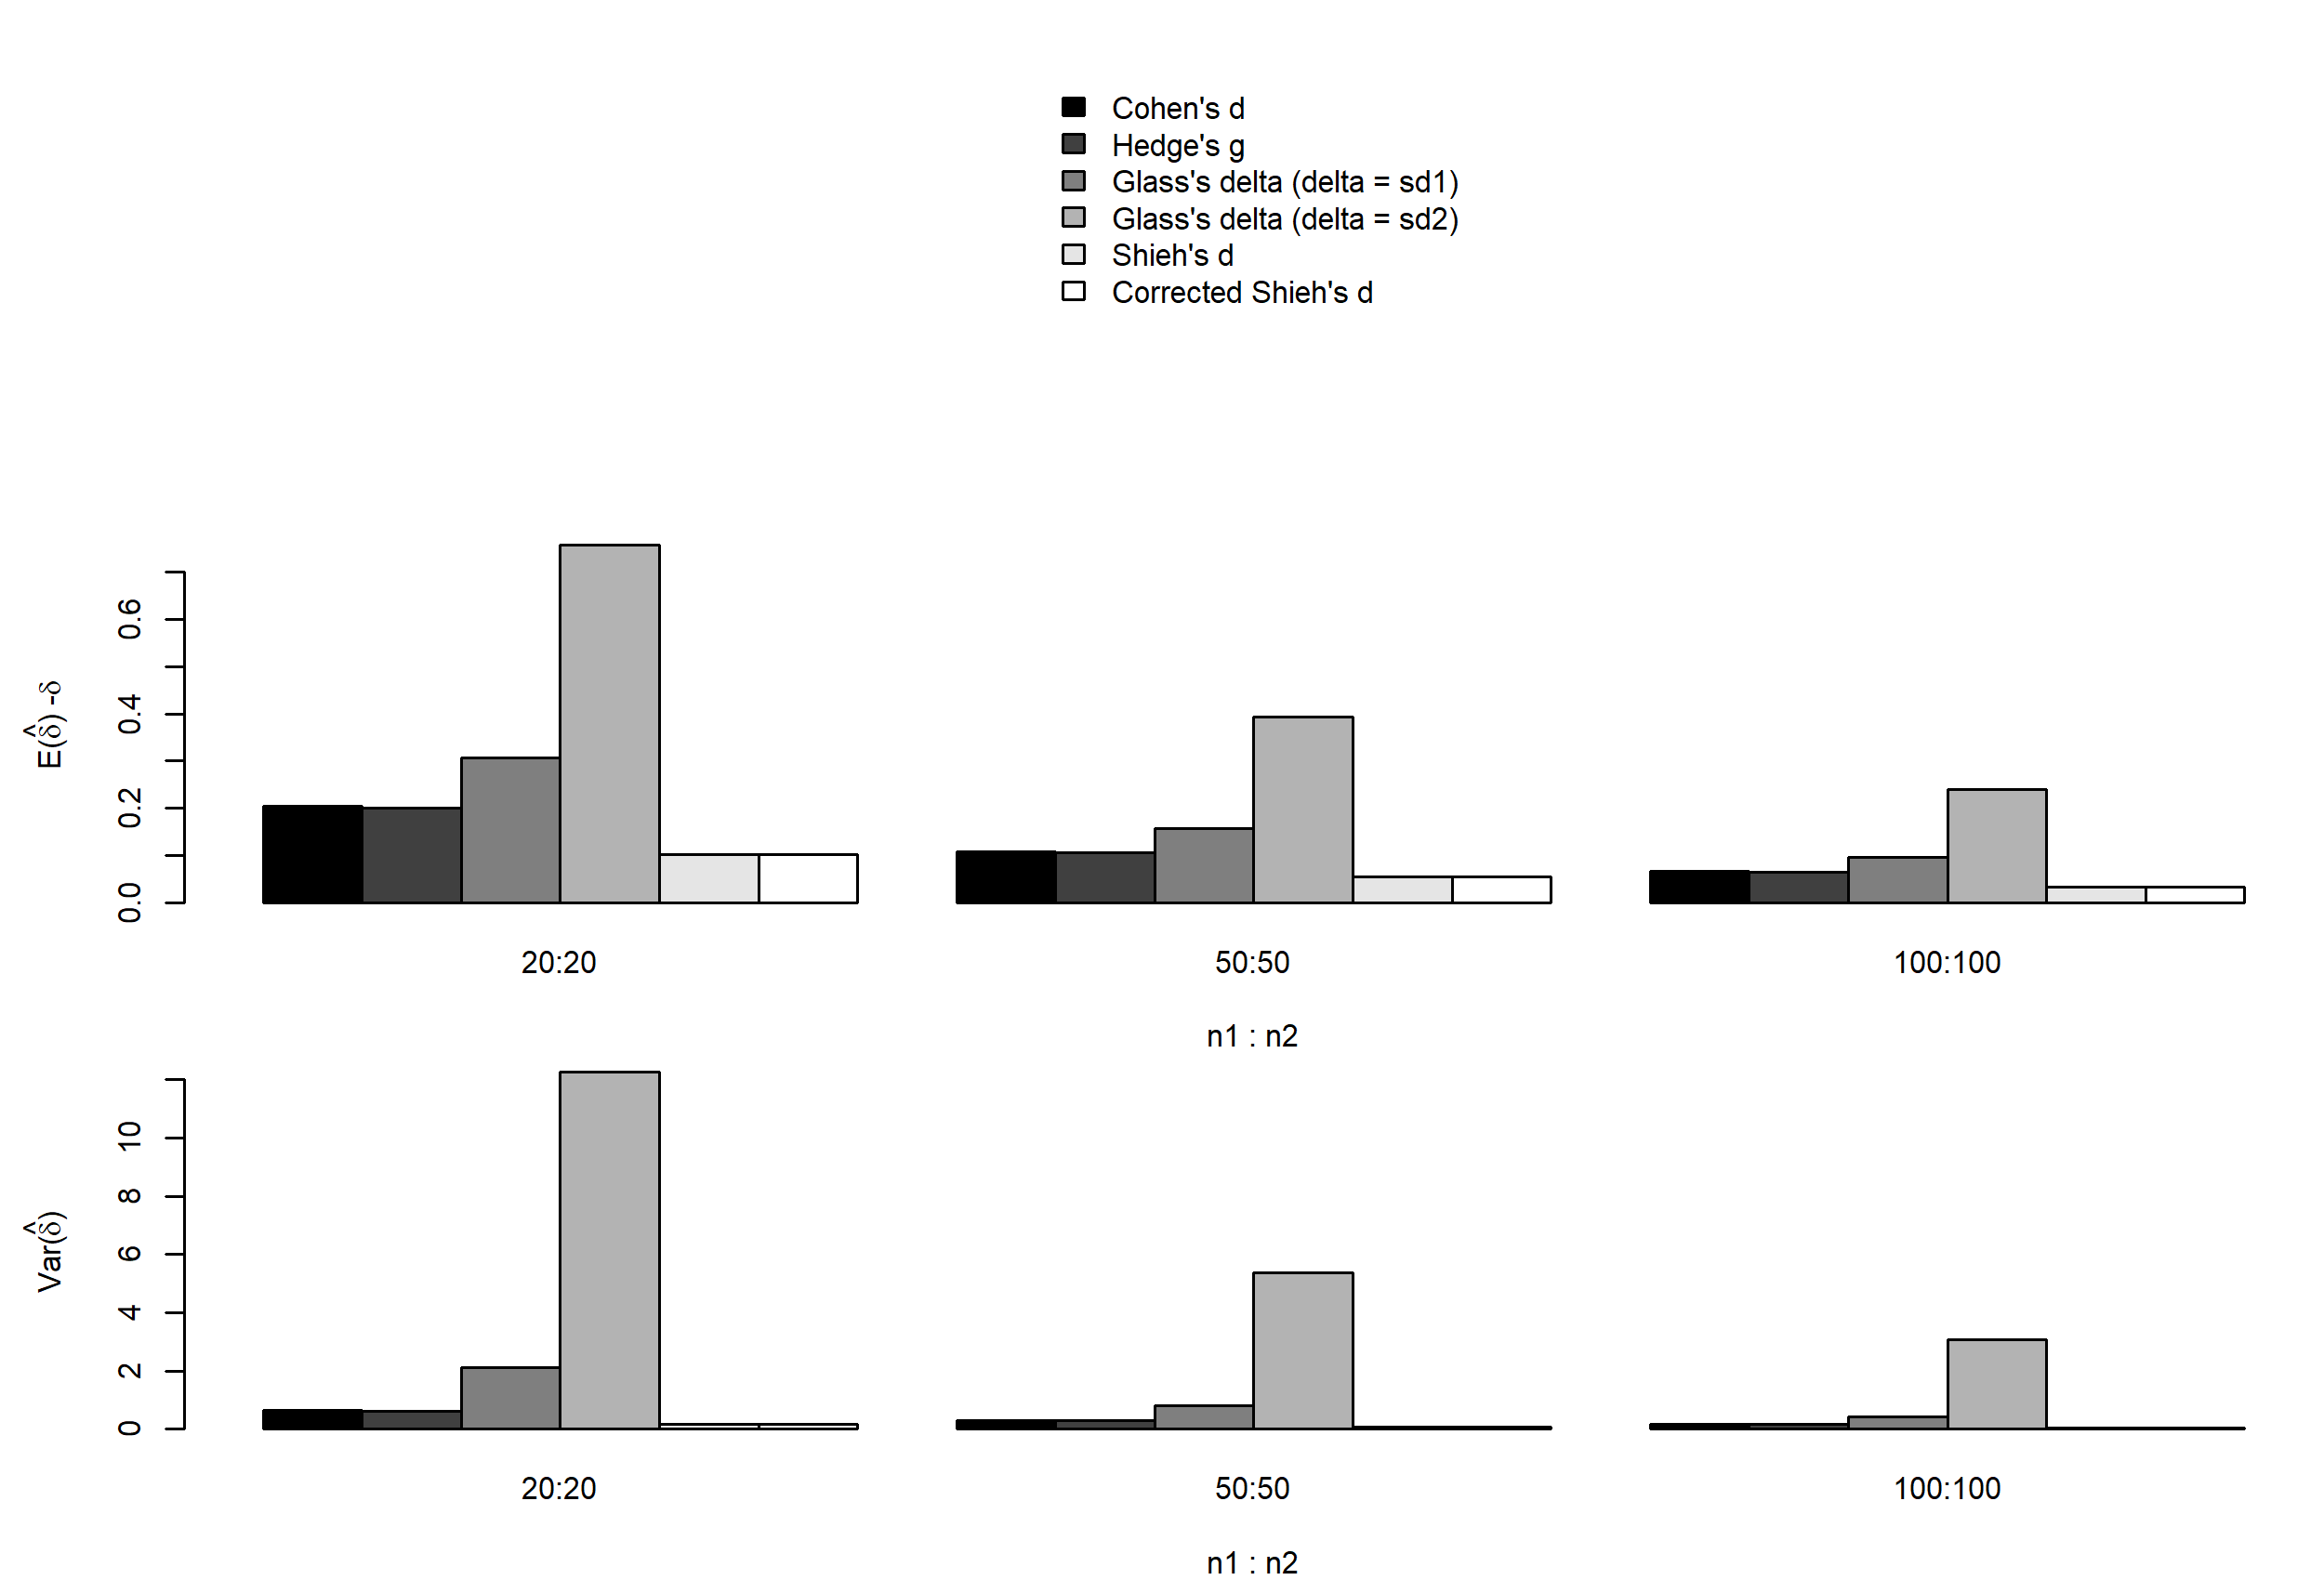
\includegraphics[width=0.2\linewidth]{C:/Users/Marie/Documents/Github_projects/Effect-sizes/Scripts outputs/Quality of ES measures/Graphs/id_Het_bal/bias_eff,G1=2.08 & G2=95.75;id_Het_bal} 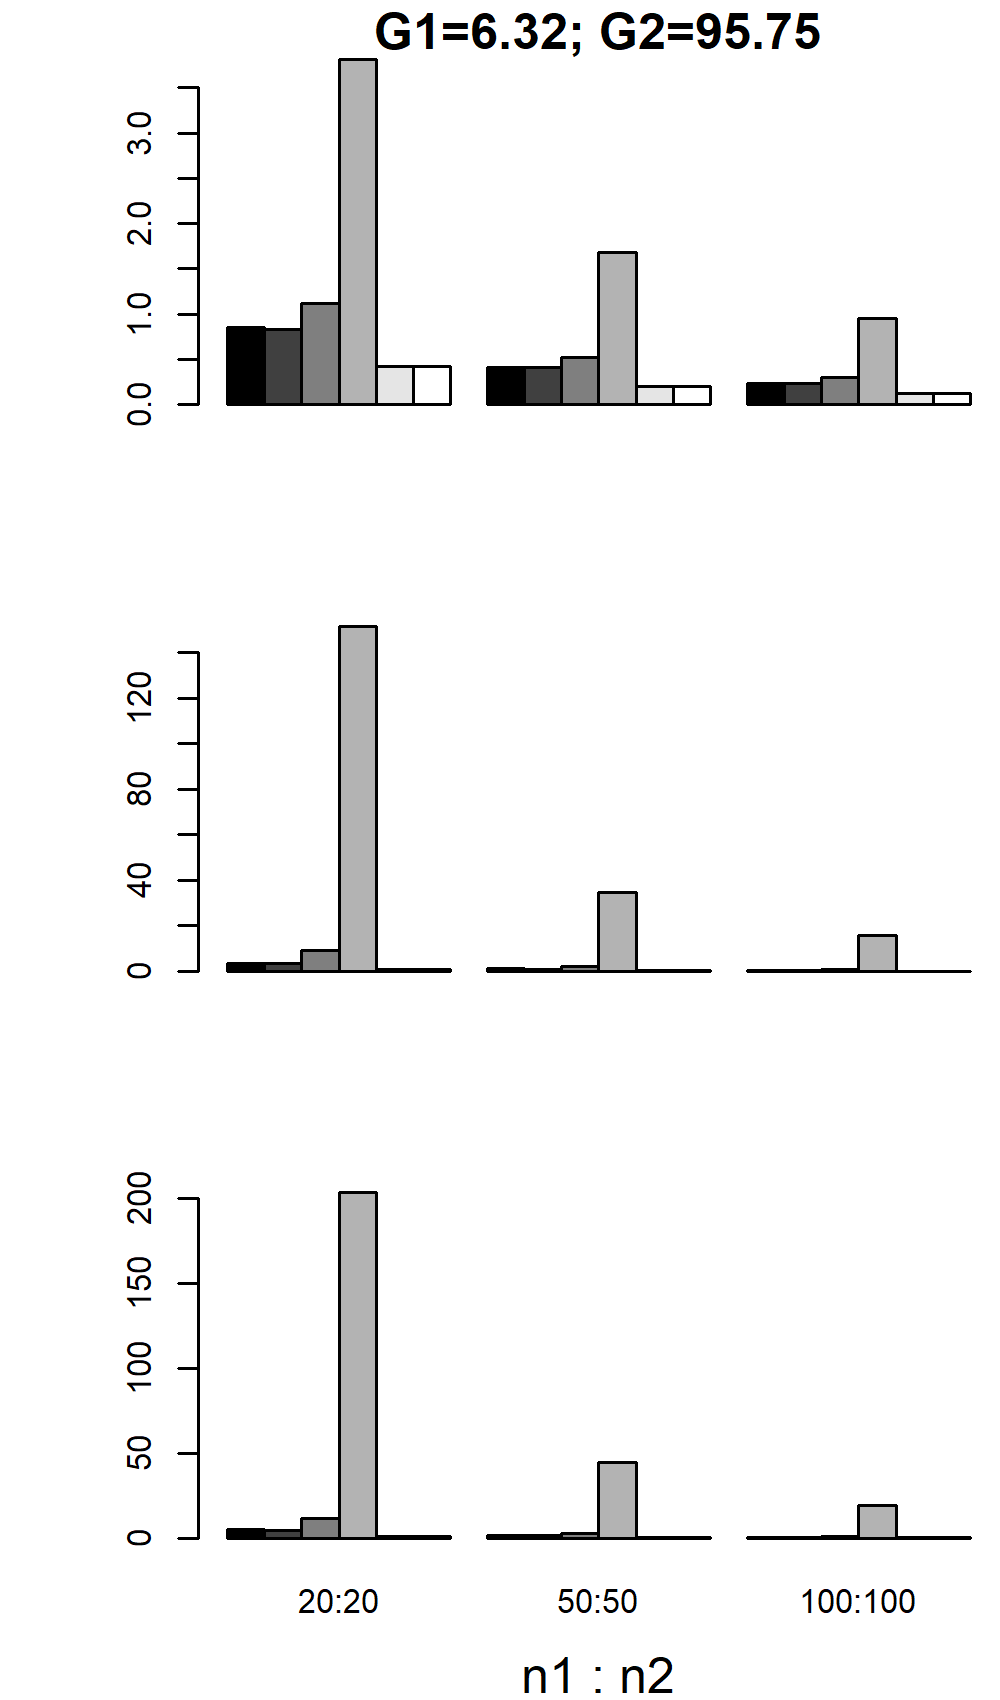
\includegraphics[width=0.2\linewidth]{C:/Users/Marie/Documents/Github_projects/Effect-sizes/Scripts outputs/Quality of ES measures/Graphs/id_Het_bal/bias_eff,G1=6.32 & G2=95.75;id_Het_bal} 

}

\caption{Bias and efficiency of five estimator of standardized mean difference, when variances are unequal across groups and sample sizes are equal (condition c)}\label{fig:idHetbal}
\end{sidewaysfigure}

Figure \ref{fig:idHomrnull} shows that when population variances are equal but sample sizes are unequal between groups, as when sample sizes were equal, while estimators are consistent, glass's \(d_s\) is generally more biased and variable that all other estimators. Again, this is due to the fact that the standardizer is estimated based on part of the total sample and unsurprisingly, the bias is even larger when choosing the \(SD\) of the smallest group as a standardizer. As long as samples are extracted from symmetric distributions, the bias and variance of glass's \(d_s\) is only a function of the sample size of the group from which standardizer is computed (because \(\sigma_1=\sigma_2\)).However, when samples are extracted from skewed distribution, because of the correlation between sample mean and sample SD, glass's \(d_s\) becomes even more biased and variable when the chosen standardizer is negatively correlated with the mean difference and associated with the smaller sample size (i.e.~when choosing \(SD_2\) as standardizer, with \(n_1 > n_2\) when distributions are right-skewed; and when choosing \(SD_1\) as standardizer, with \(n_1 < n_2\) when distributions are left-skewed). \footnote{again, remind that in all our simulations, the population mean difference is positive. If mean difference were negative, glass's $d_s$ would be more biased and variable when the chosen standardizer is positively correlated with the mean difference and associated with the smaller sample size}.

As previously, the bias of Shieh's \(d_s\) is smaller than the Cohen's \(d_s\) one (as well as the Hedge's \(g_s\) one). However, the difference is smaller than previously. Remember that when sample sizes differ between groups, Shieh's \(d_s\) is always more than twice smaller than Cohen's \(d_s\) (see Appendix 1 for more details). As a consequence, if both Cohen's \(d_s\) and Shieh's \(d_s\) performed as well, the bias of Shieh's \(d_s\) should be more than twice smaller than Cohen's \(d_s\) bias (and the variance of Shieh's \(d_s\) should be more than four time smaller than Cohen's \(d_s\) bias), but it's not. It's confirmed by the second and fourth rows in Figure \ref{fig:idHomrnull} where we can see that the relative bias and variance of Shieh's \(d_s\) are larger than the relative bias and variance of Cohen's \(d_s\), that remains the best indicator in terms of bias. However, it is very interesting to note that our transformed Shieh's \(d^*_s\) is on average less biased and variable than original Shieh's \(d_s\), both if raw and relative terms. This measure seems to perform almost as well as Cohen's \(d_s\).

\begin{sidewaysfigure}

{\centering 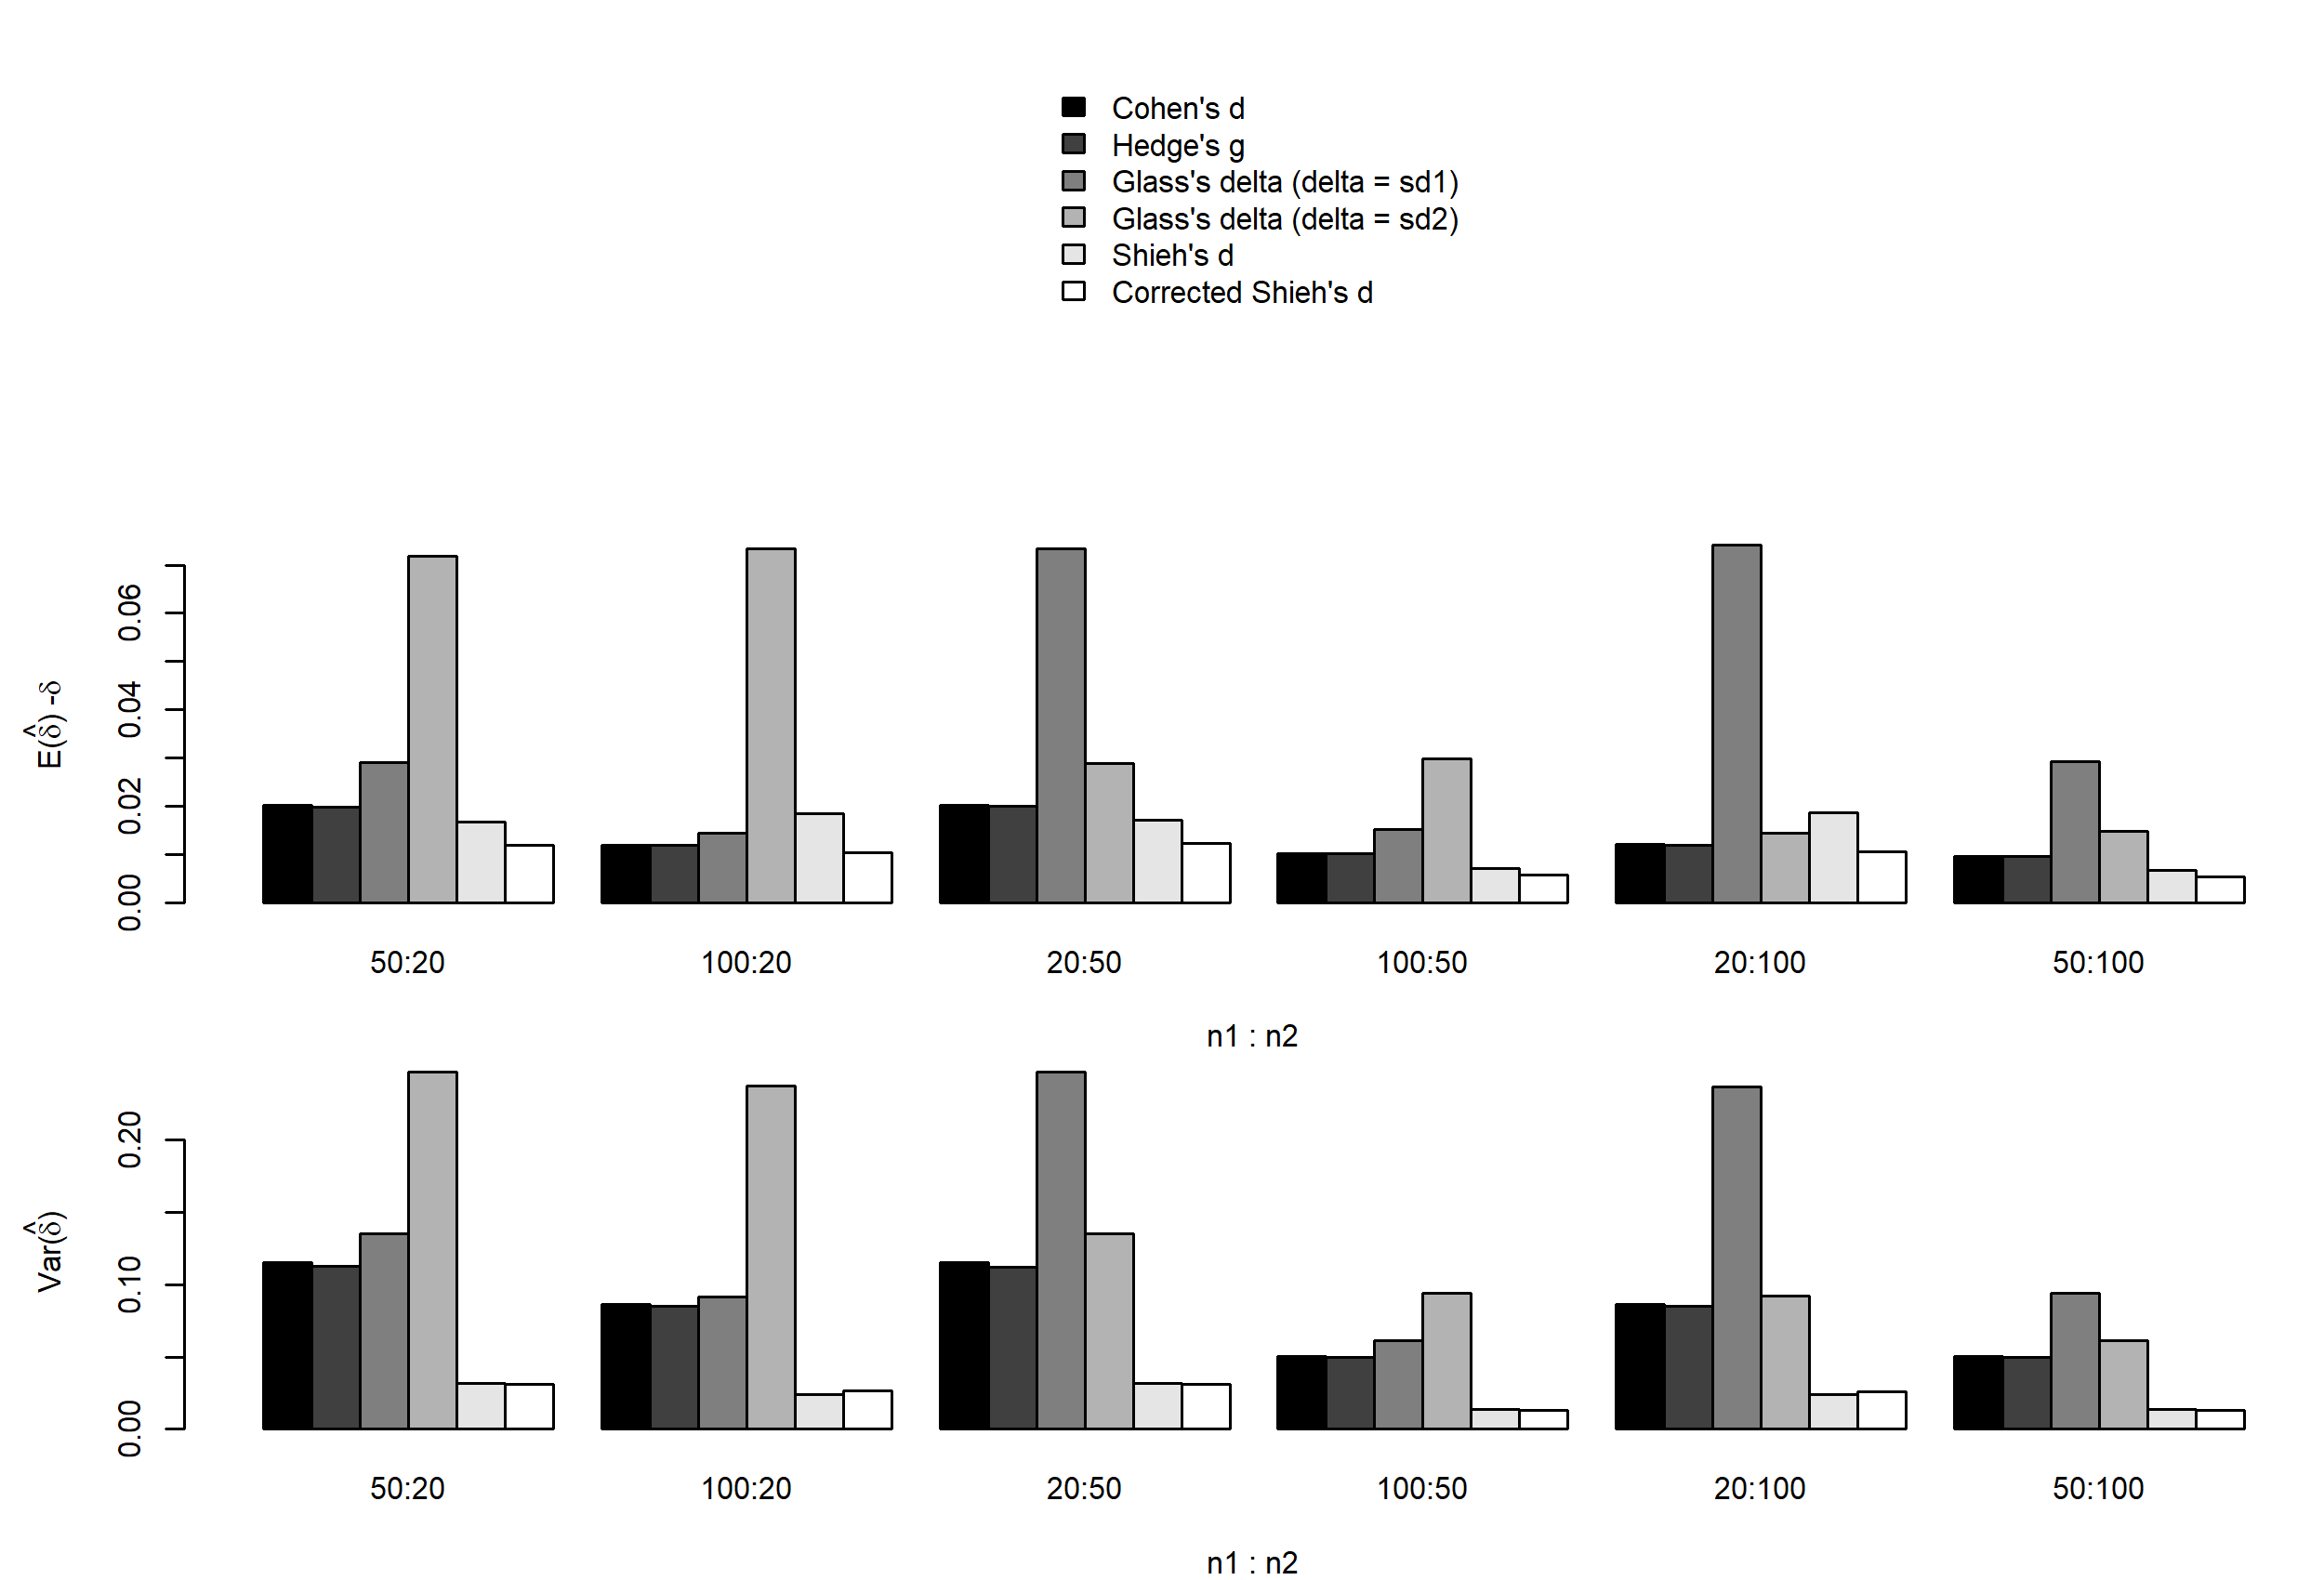
\includegraphics[width=0.2\linewidth]{C:/Users/Marie/Documents/Github_projects/Effect-sizes/Scripts outputs/Quality of ES measures/Graphs/id_Hom_rnull/bias_eff,G1=0 & G2=0;id_Hom_rnull} 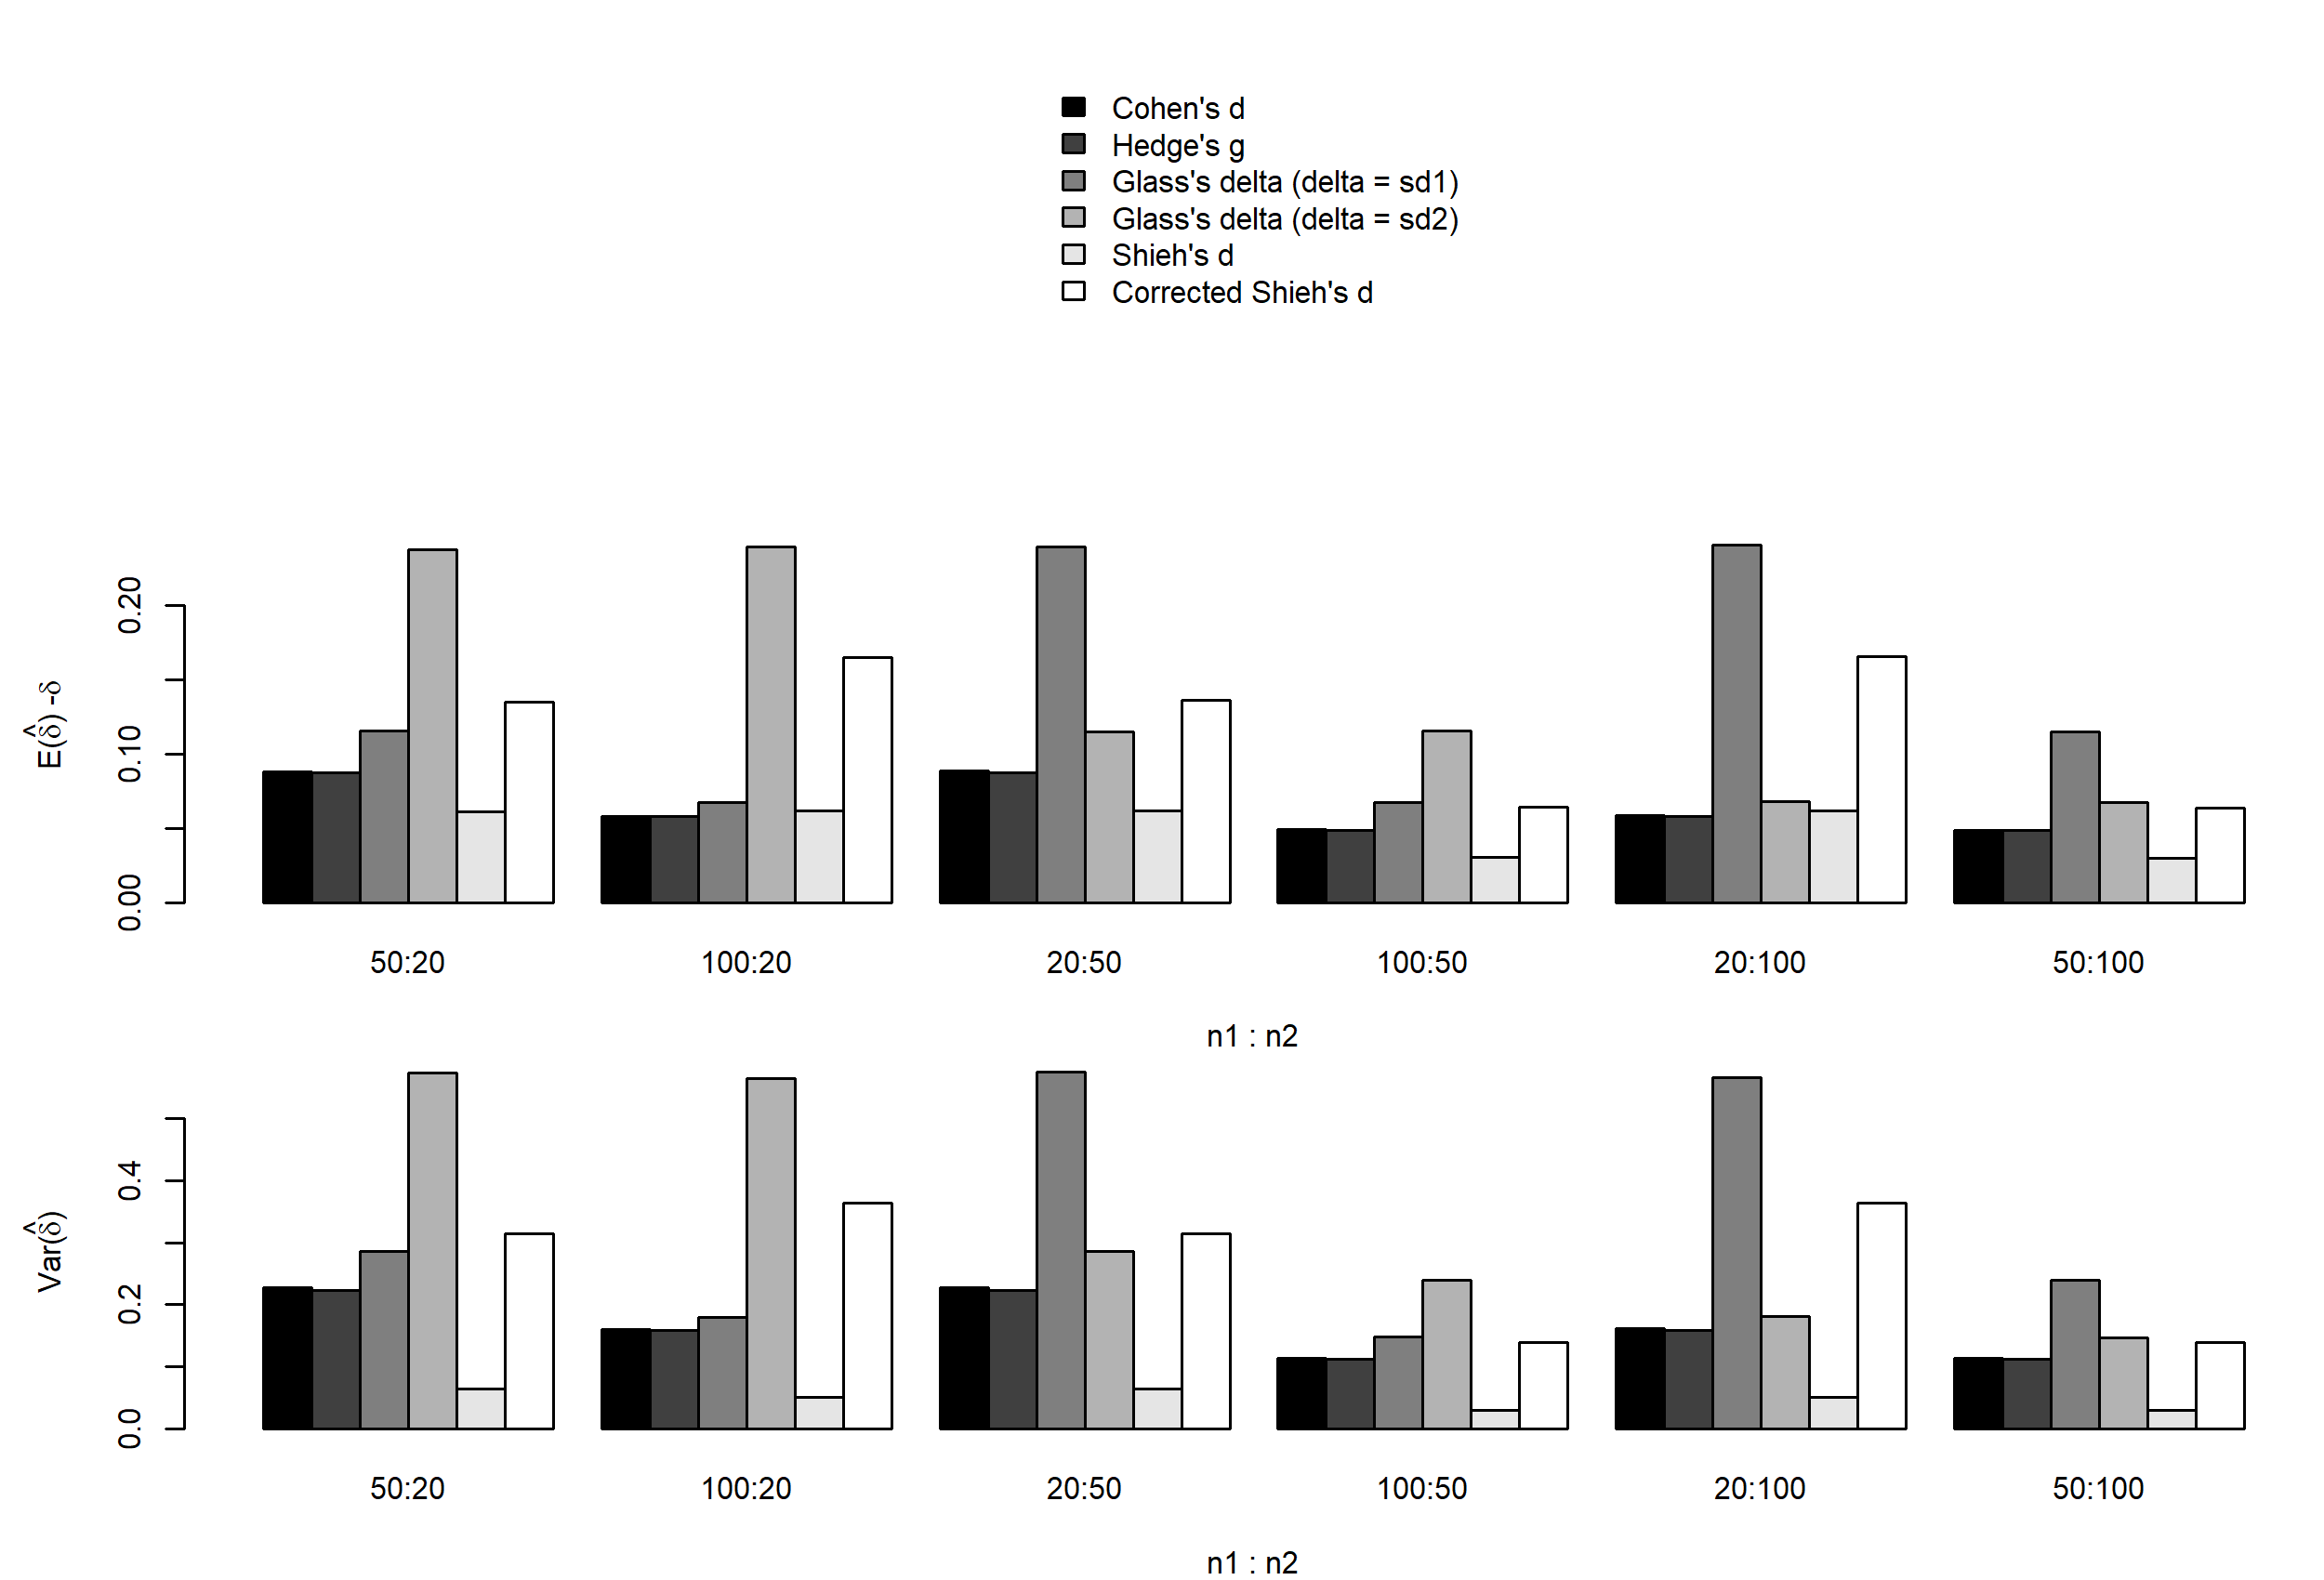
\includegraphics[width=0.2\linewidth]{C:/Users/Marie/Documents/Github_projects/Effect-sizes/Scripts outputs/Quality of ES measures/Graphs/id_Hom_rnull/bias_eff,G1=0 & G2=95.75;id_Hom_rnull} 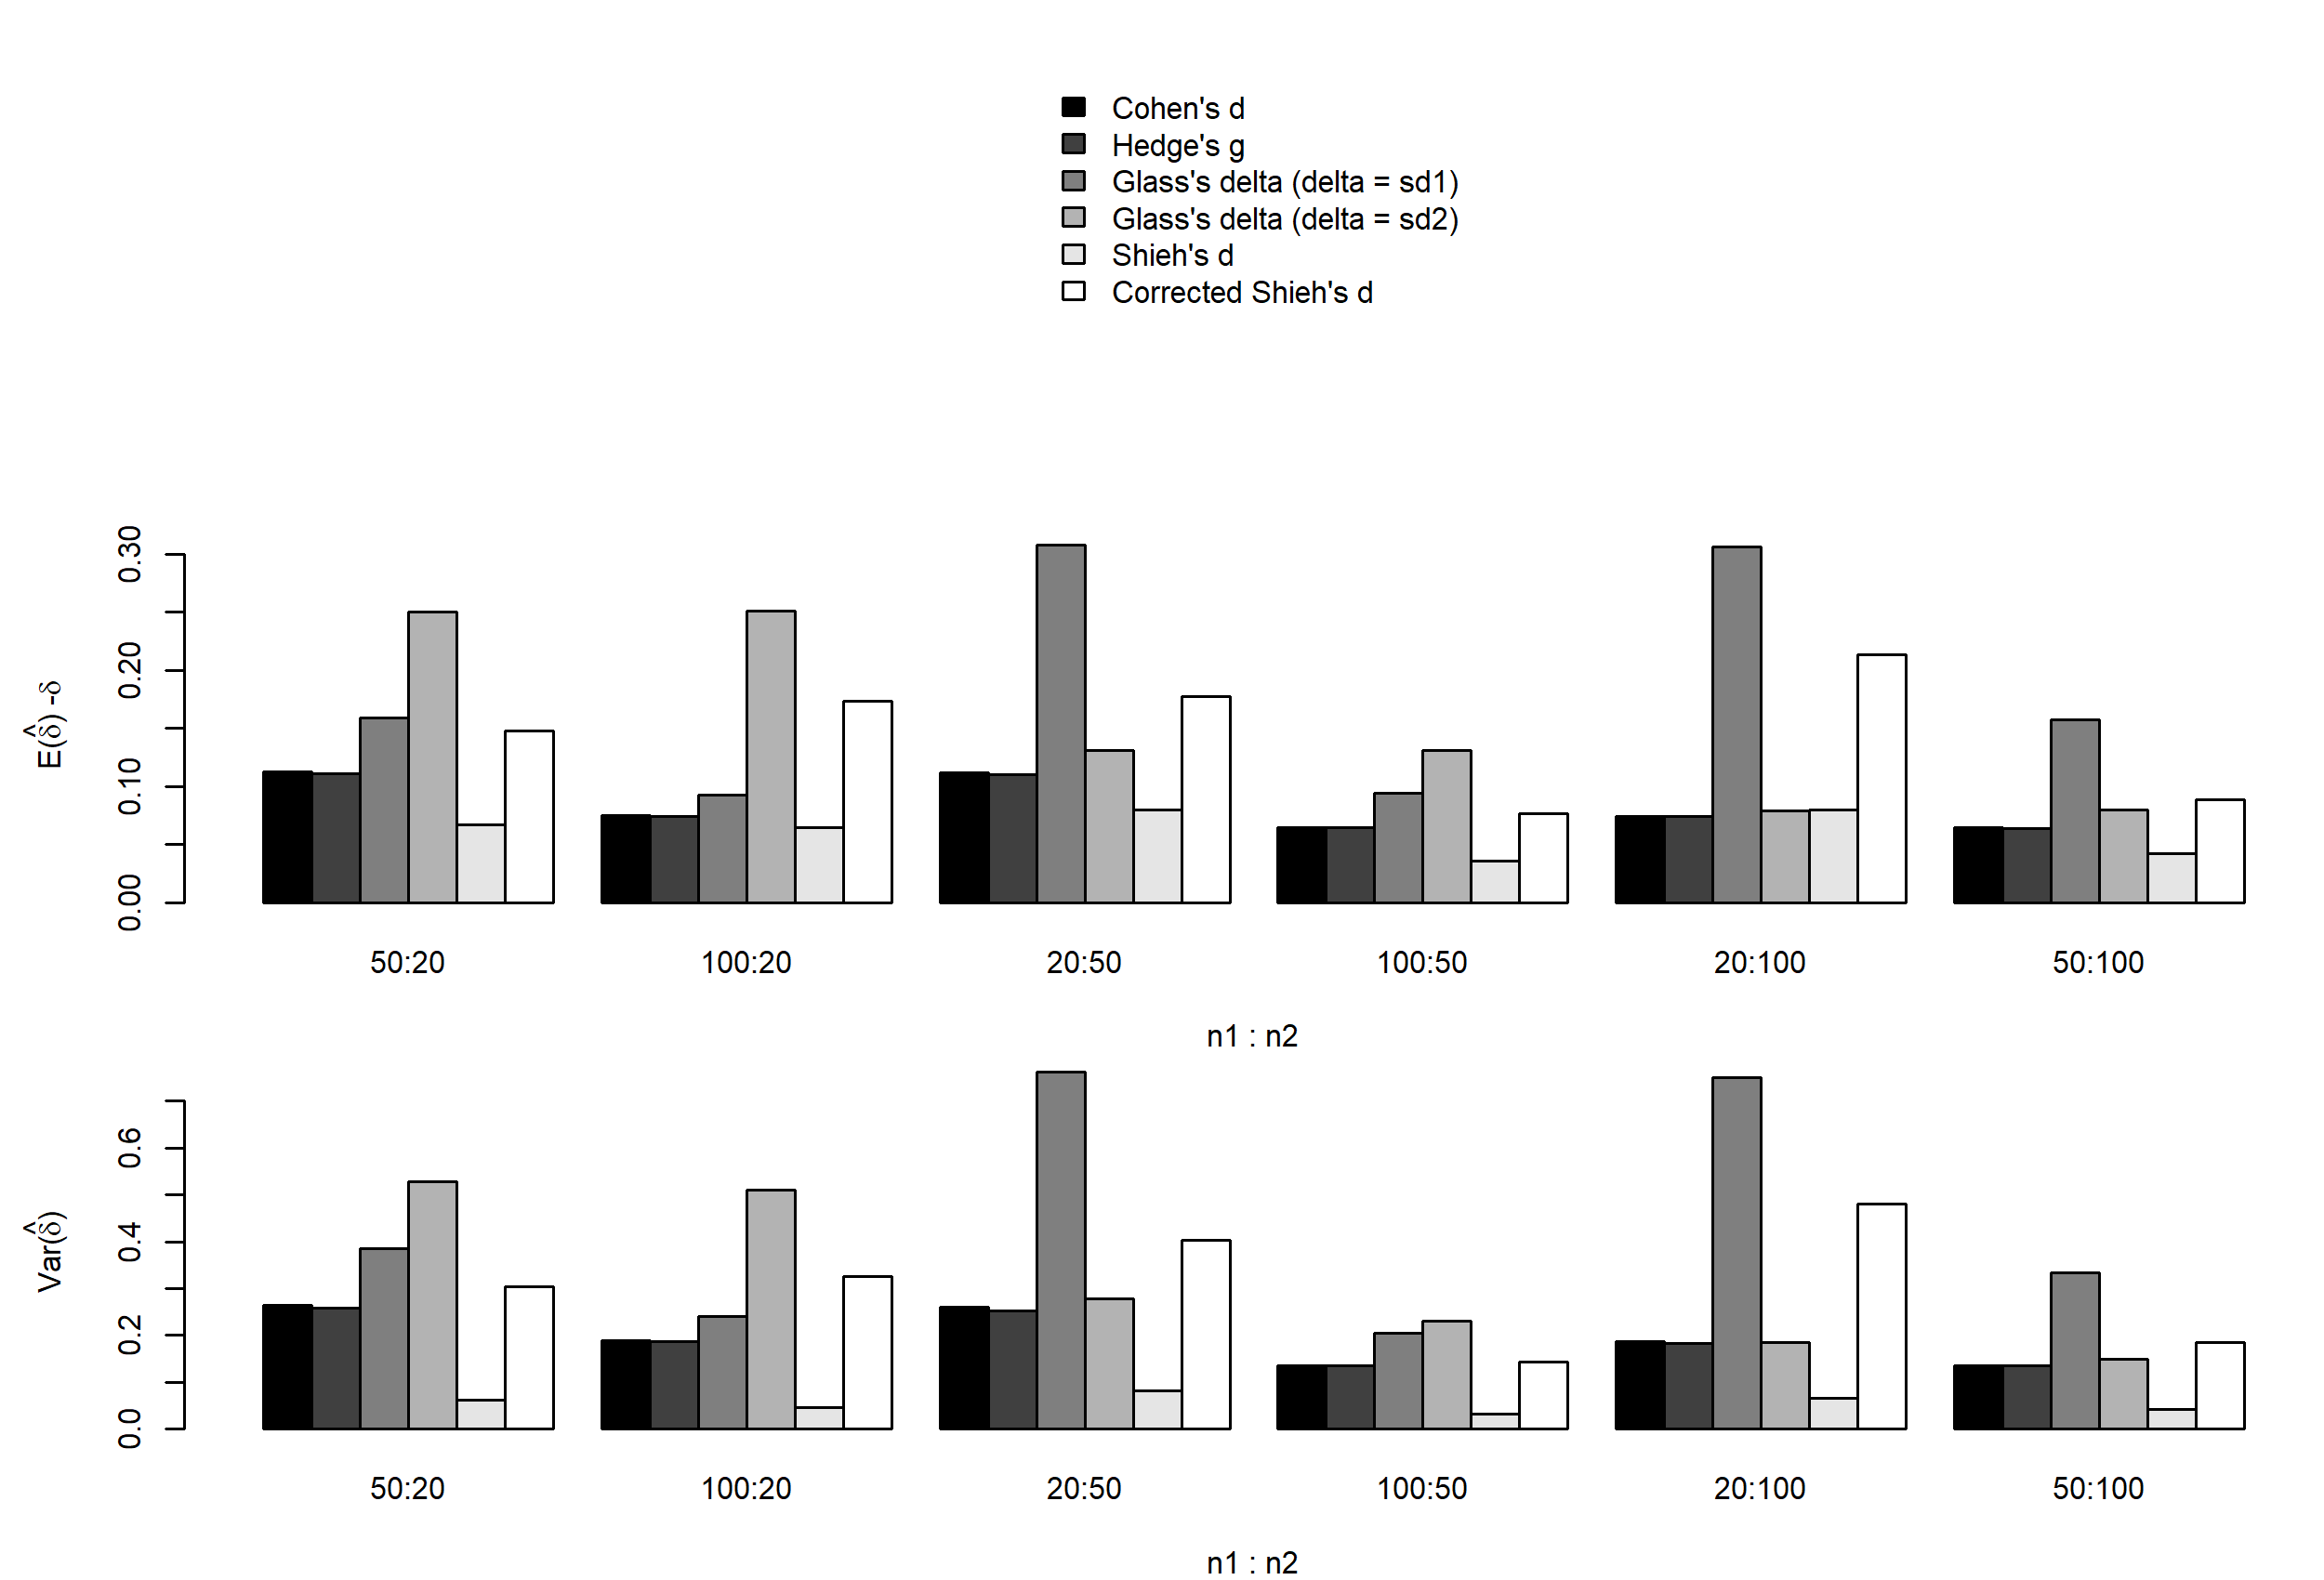
\includegraphics[width=0.2\linewidth]{C:/Users/Marie/Documents/Github_projects/Effect-sizes/Scripts outputs/Quality of ES measures/Graphs/id_Hom_rnull/bias_eff,G1=2.08 & G2=95.75;id_Hom_rnull} 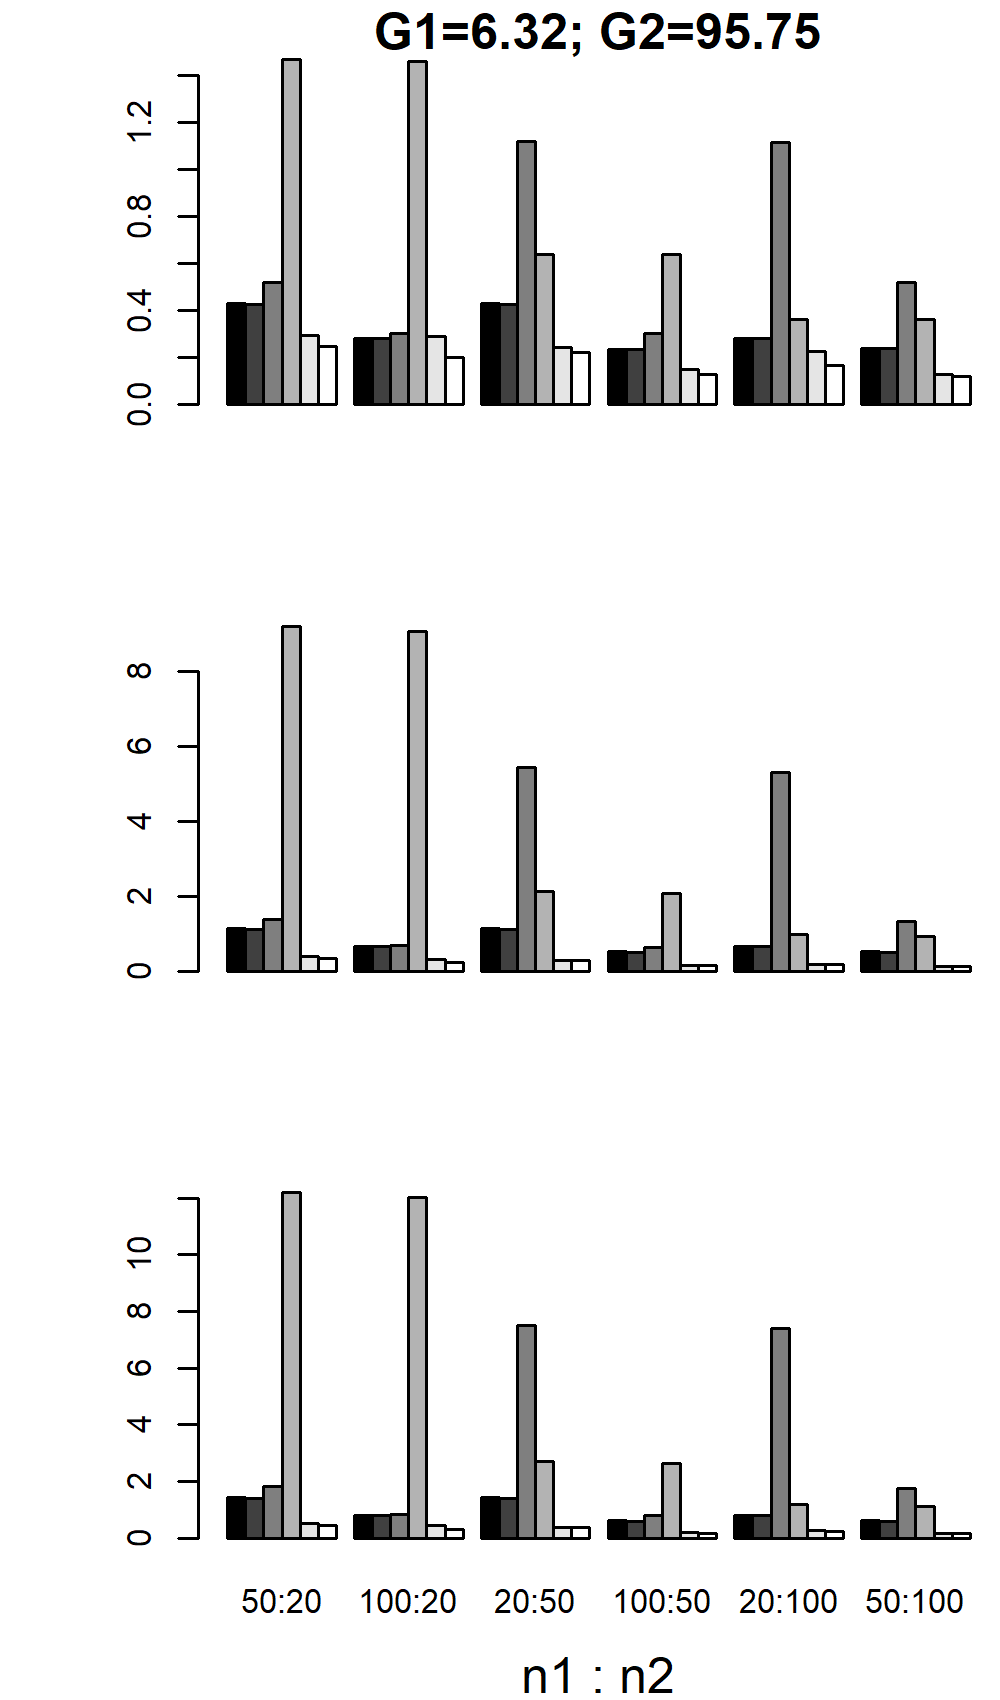
\includegraphics[width=0.2\linewidth]{C:/Users/Marie/Documents/Github_projects/Effect-sizes/Scripts outputs/Quality of ES measures/Graphs/id_Hom_rnull/bias_eff,G1=6.32 & G2=95.75;id_Hom_rnull} 

}

\caption{Bias and efficiency of five estimator of standardized mean difference, when variances are equal across groups and sample sizes are unequal}\label{fig:idHomrnull}
\end{sidewaysfigure}

Figure \ref{fig:idHetrpos} and \ref{fig:idHetrneg} refer to conditions where there is a pairing between population variances and sample sizes. We know that in these configurations, the pooled variance will be poorly estimated (see the second remark at the beginning of the result section), and therefore, we will not discuss the Cohen's \(d_s\) and Hedge's \(g_s\).We will only compare the performance of Glass's \(d_s\), Shieh's \(d_s\) and Shieh's \(d^*_s\).

Figure \ref{fig:idHetrpos} shows that when variances are unequal, and the largest group is associated with largest variance, the more biased and variable estimator is Glass's \(d_s\) when choosing the standard deviation of the smallest group as standardizer.
REM: AGAIN ONE OBSERVE THE SAME INTERACTION EFFECT BETWEEN STANDARDISER IN GLASS MEASURE AND SENSE OF ASYMMETRY AS OBSERVED FOR FIGURE 3 (IN SAME DIRECTION: WITH NEGATIVE SKEWNESS, WORST WHEN CHOOSING SD1 AND WHEN POSITIVE SKEWNESS, WORST WHEN CHOOSING SD2). Glass's \(d_s\) when choosing the standard deviation of the largest group as standardizer, Shieh's \(d_s\) and transformed Shieh's \(d^*_s\) perform very similarly, both in terms of bias and efficiency.

\begin{sidewaysfigure}

{\centering 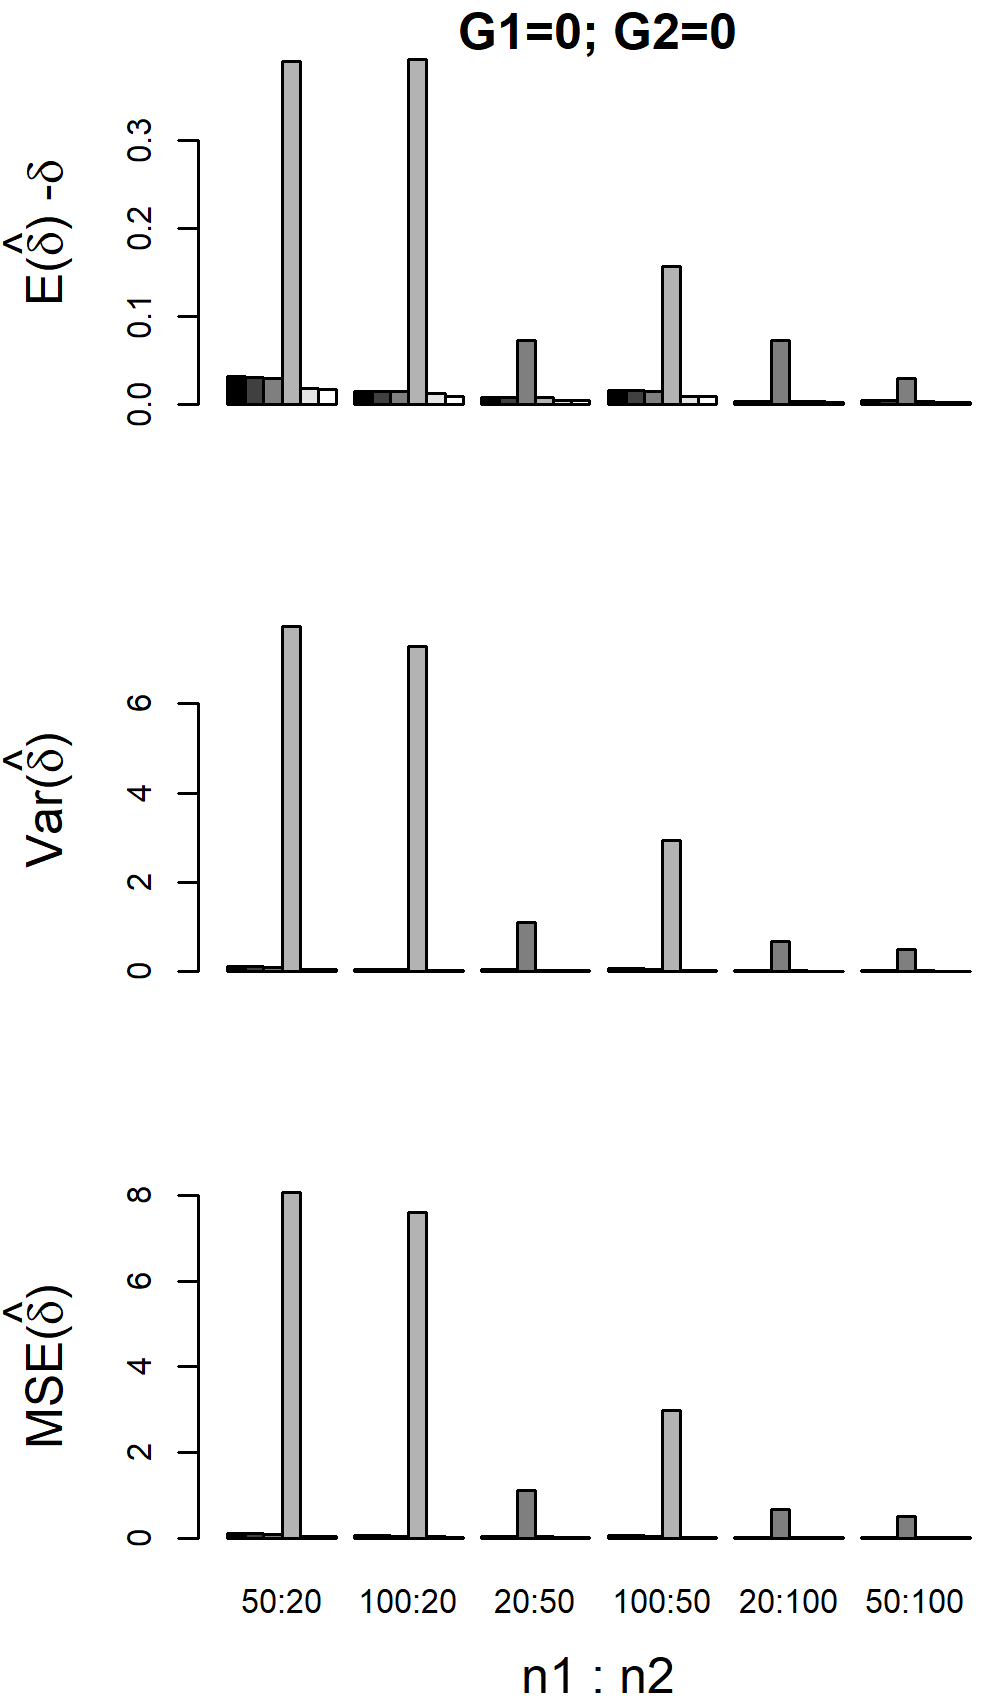
\includegraphics[width=0.2\linewidth]{C:/Users/Marie/Documents/Github_projects/Effect-sizes/Scripts outputs/Quality of ES measures/Graphs/id_Het_rpos/bias_eff,G1=0 & G2=0;id_Het_rpos} 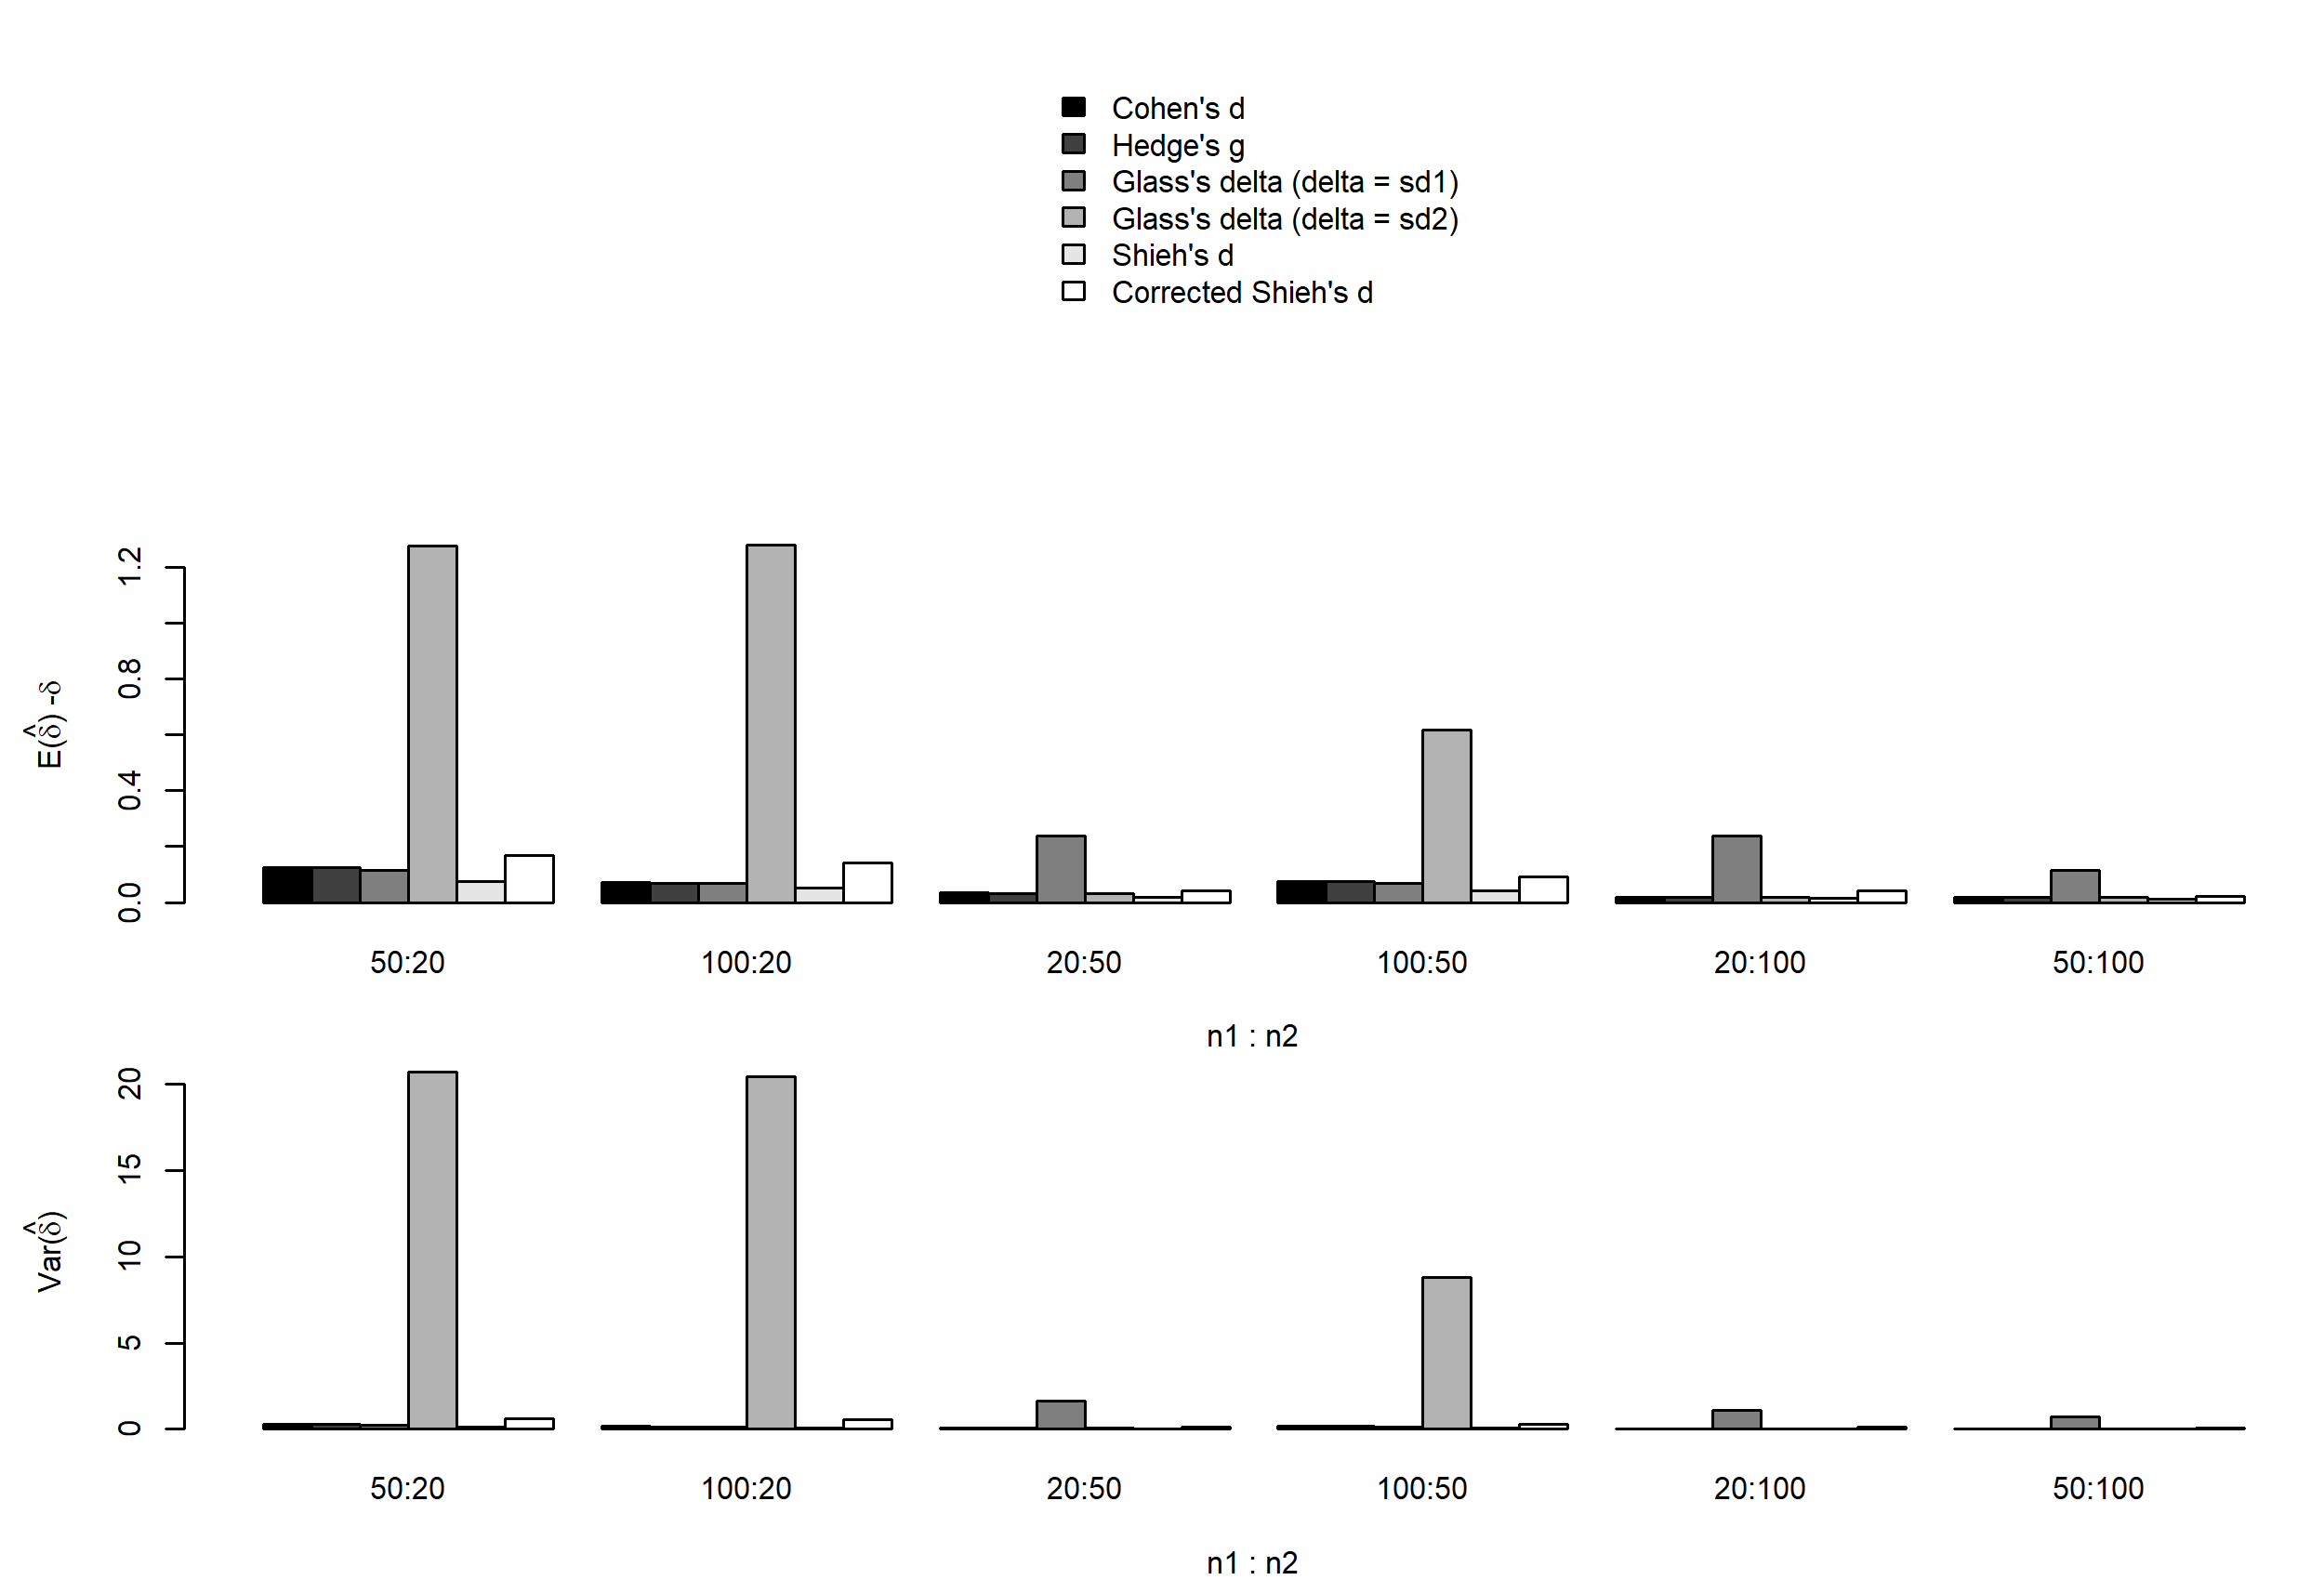
\includegraphics[width=0.2\linewidth]{C:/Users/Marie/Documents/Github_projects/Effect-sizes/Scripts outputs/Quality of ES measures/Graphs/id_Het_rpos/bias_eff,G1=0 & G2=95.75;id_Het_rpos} 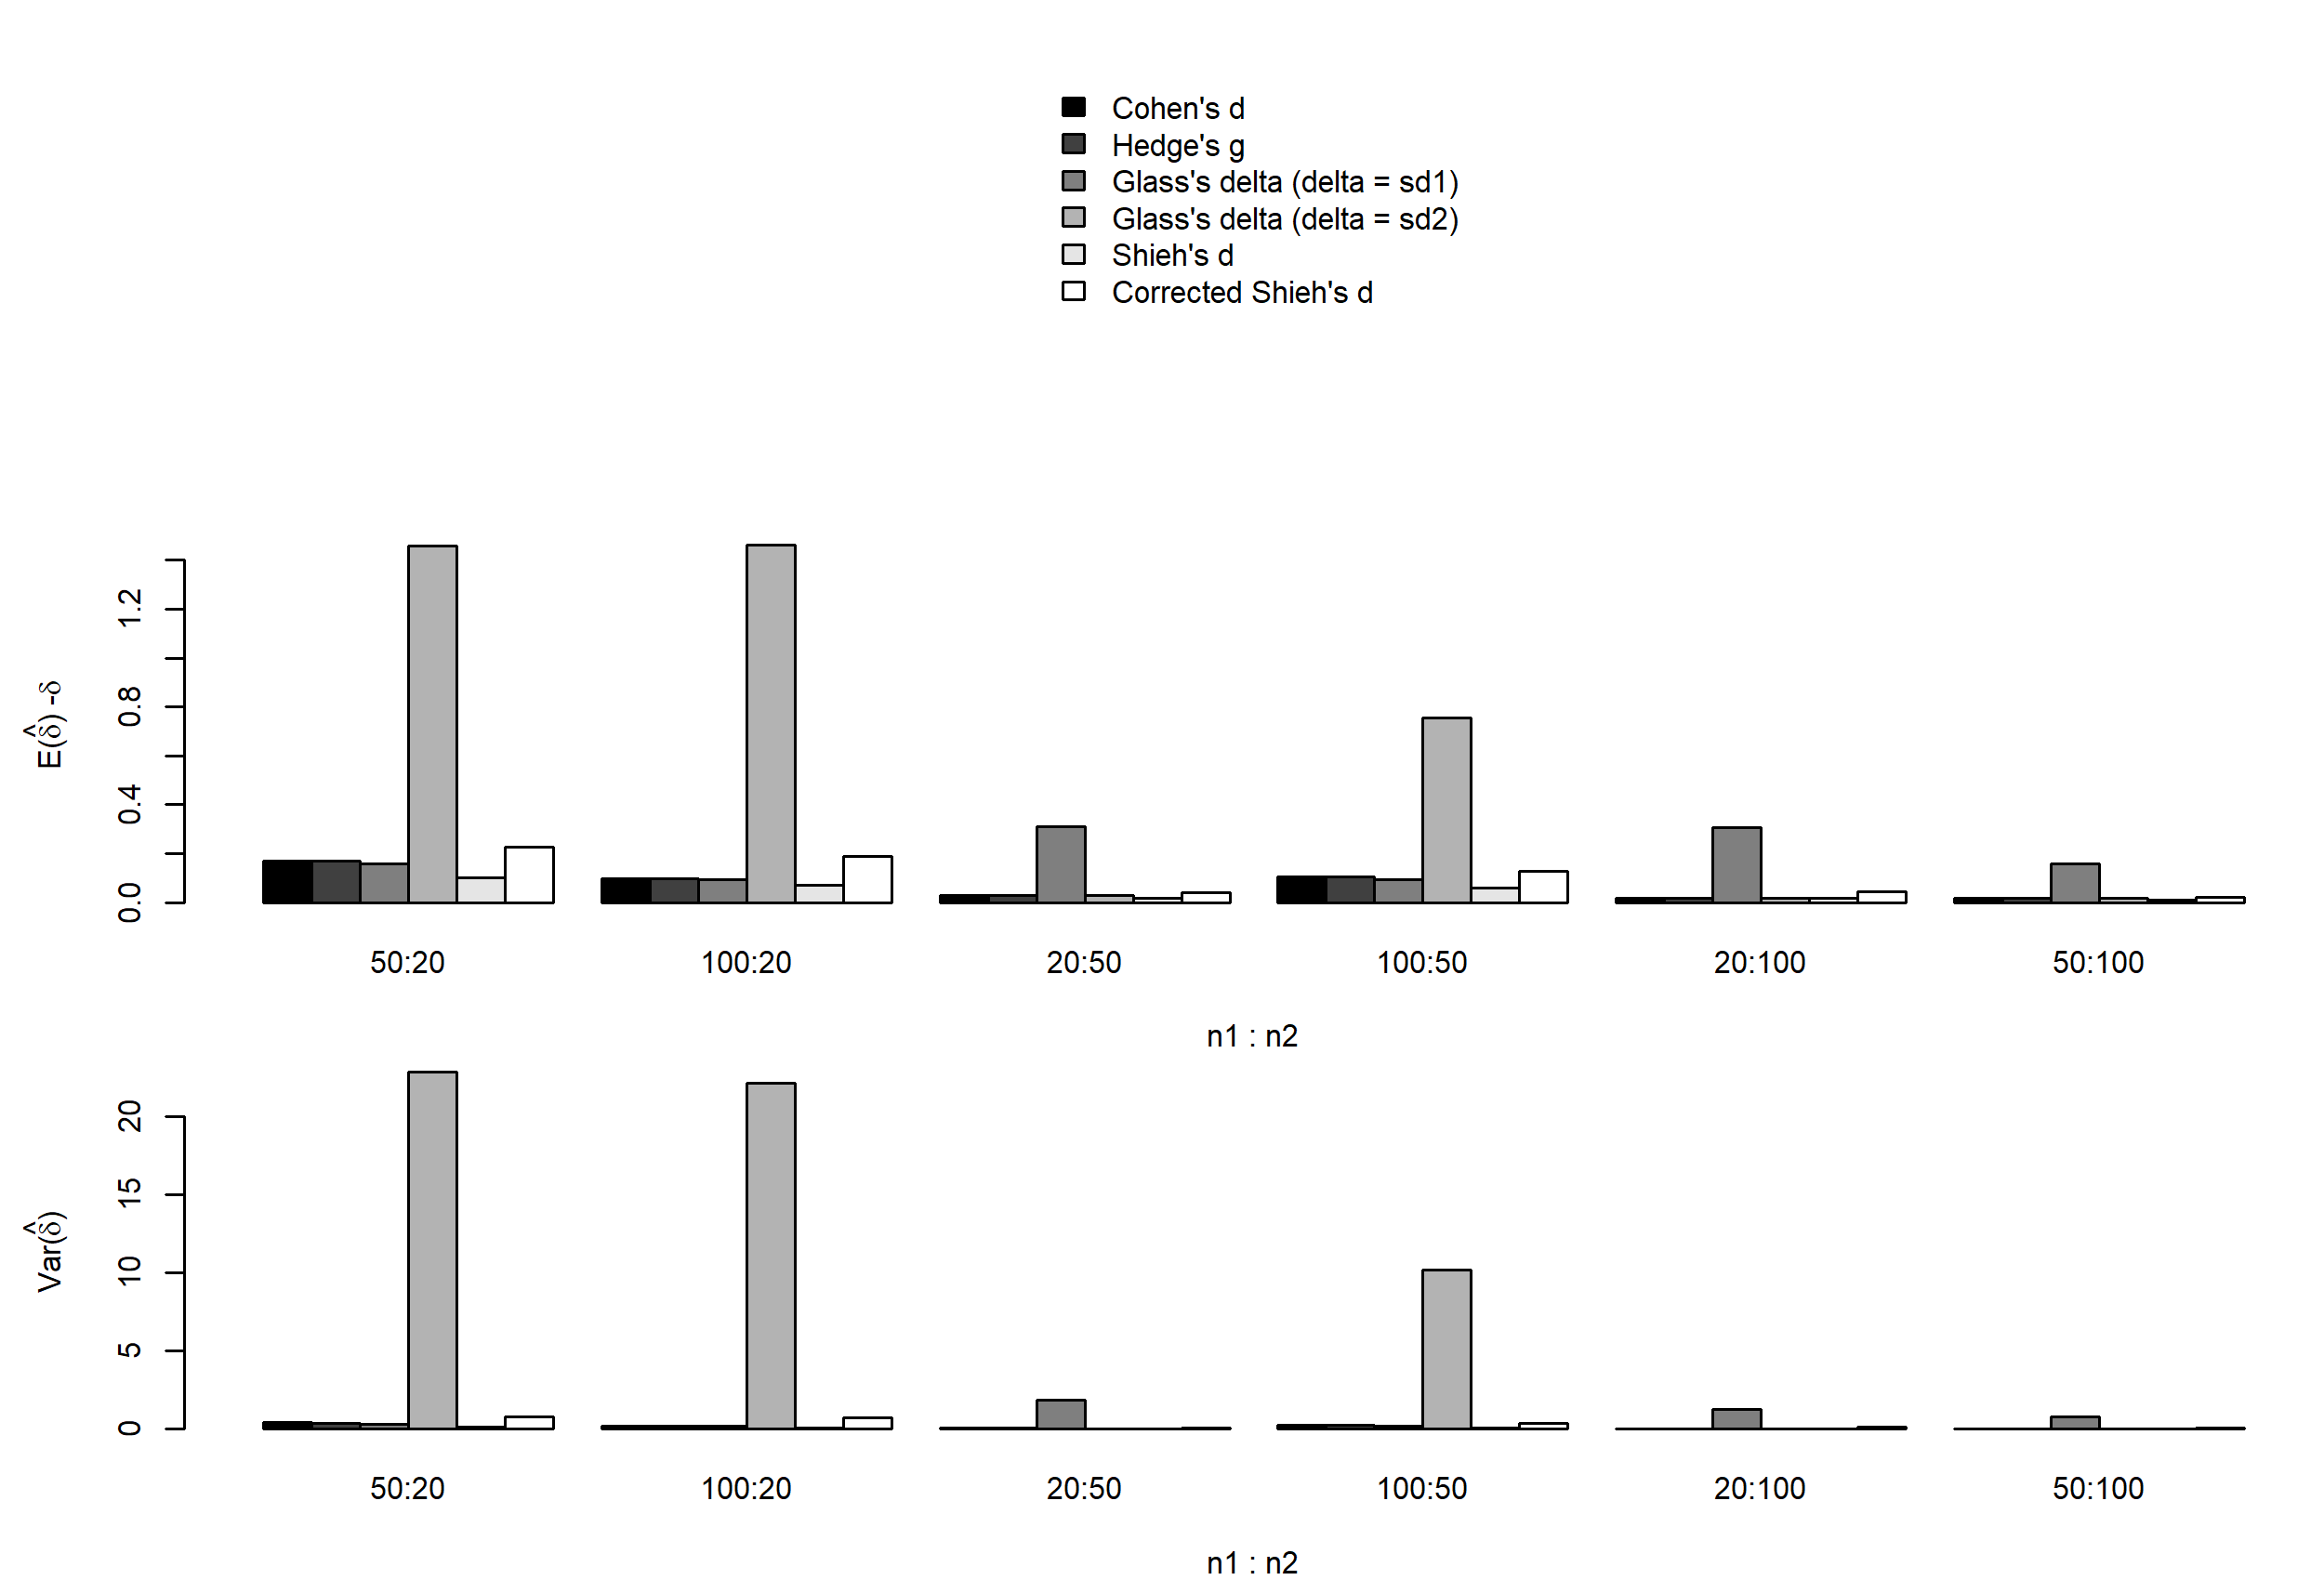
\includegraphics[width=0.2\linewidth]{C:/Users/Marie/Documents/Github_projects/Effect-sizes/Scripts outputs/Quality of ES measures/Graphs/id_Het_rpos/bias_eff,G1=2.08 & G2=95.75;id_Het_rpos} 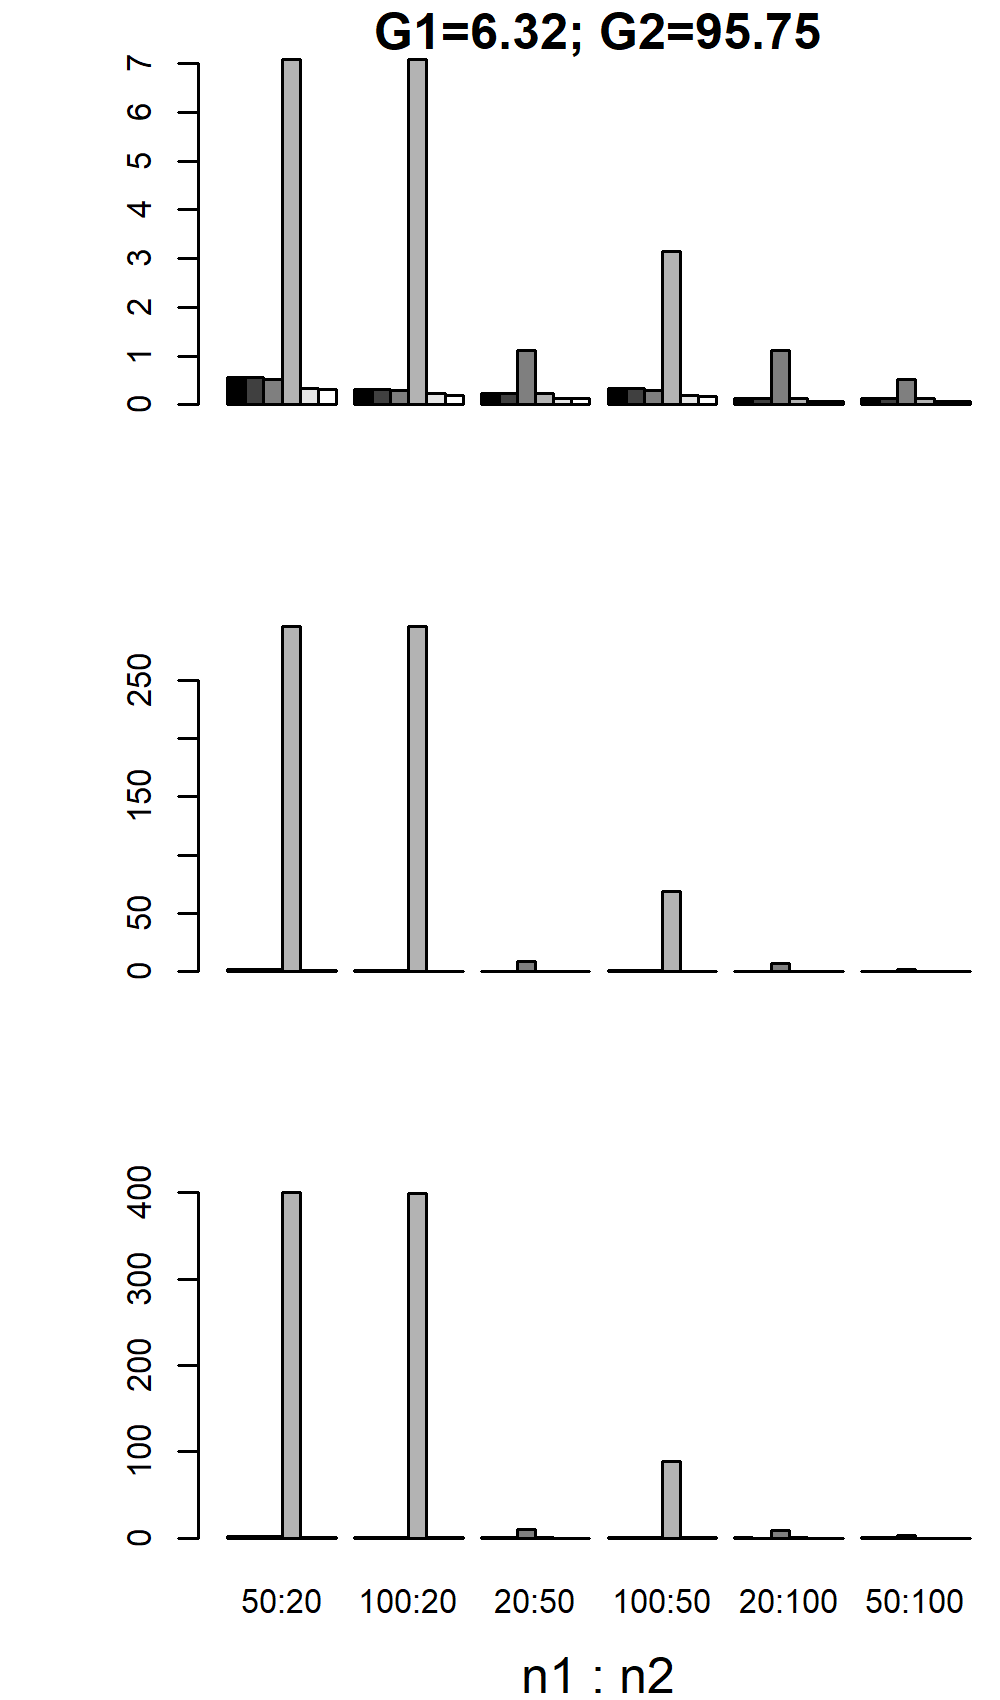
\includegraphics[width=0.2\linewidth]{C:/Users/Marie/Documents/Github_projects/Effect-sizes/Scripts outputs/Quality of ES measures/Graphs/id_Het_rpos/bias_eff,G1=6.32 & G2=95.75;id_Het_rpos} 

}

\caption{Bias and efficiency of five estimator of standardized mean difference, when variances and sample sizes are unequal across groups, with positive correlation between them}\label{fig:idHetrpos}
\end{sidewaysfigure}

Figure \ref{fig:idHetrneg} shows that when variances are unequal, and the largest group is associated with smallest variance, as in all other configurations, the more biased and variable estimator is Glass's \(d_s\) when choosing the standard deviation of the smallest group as standardizer (sauf quand asymetrie négative\ldots{} not true anymore when there is asymmetry\ldots{} explain it).

\begin{sidewaysfigure}

{\centering 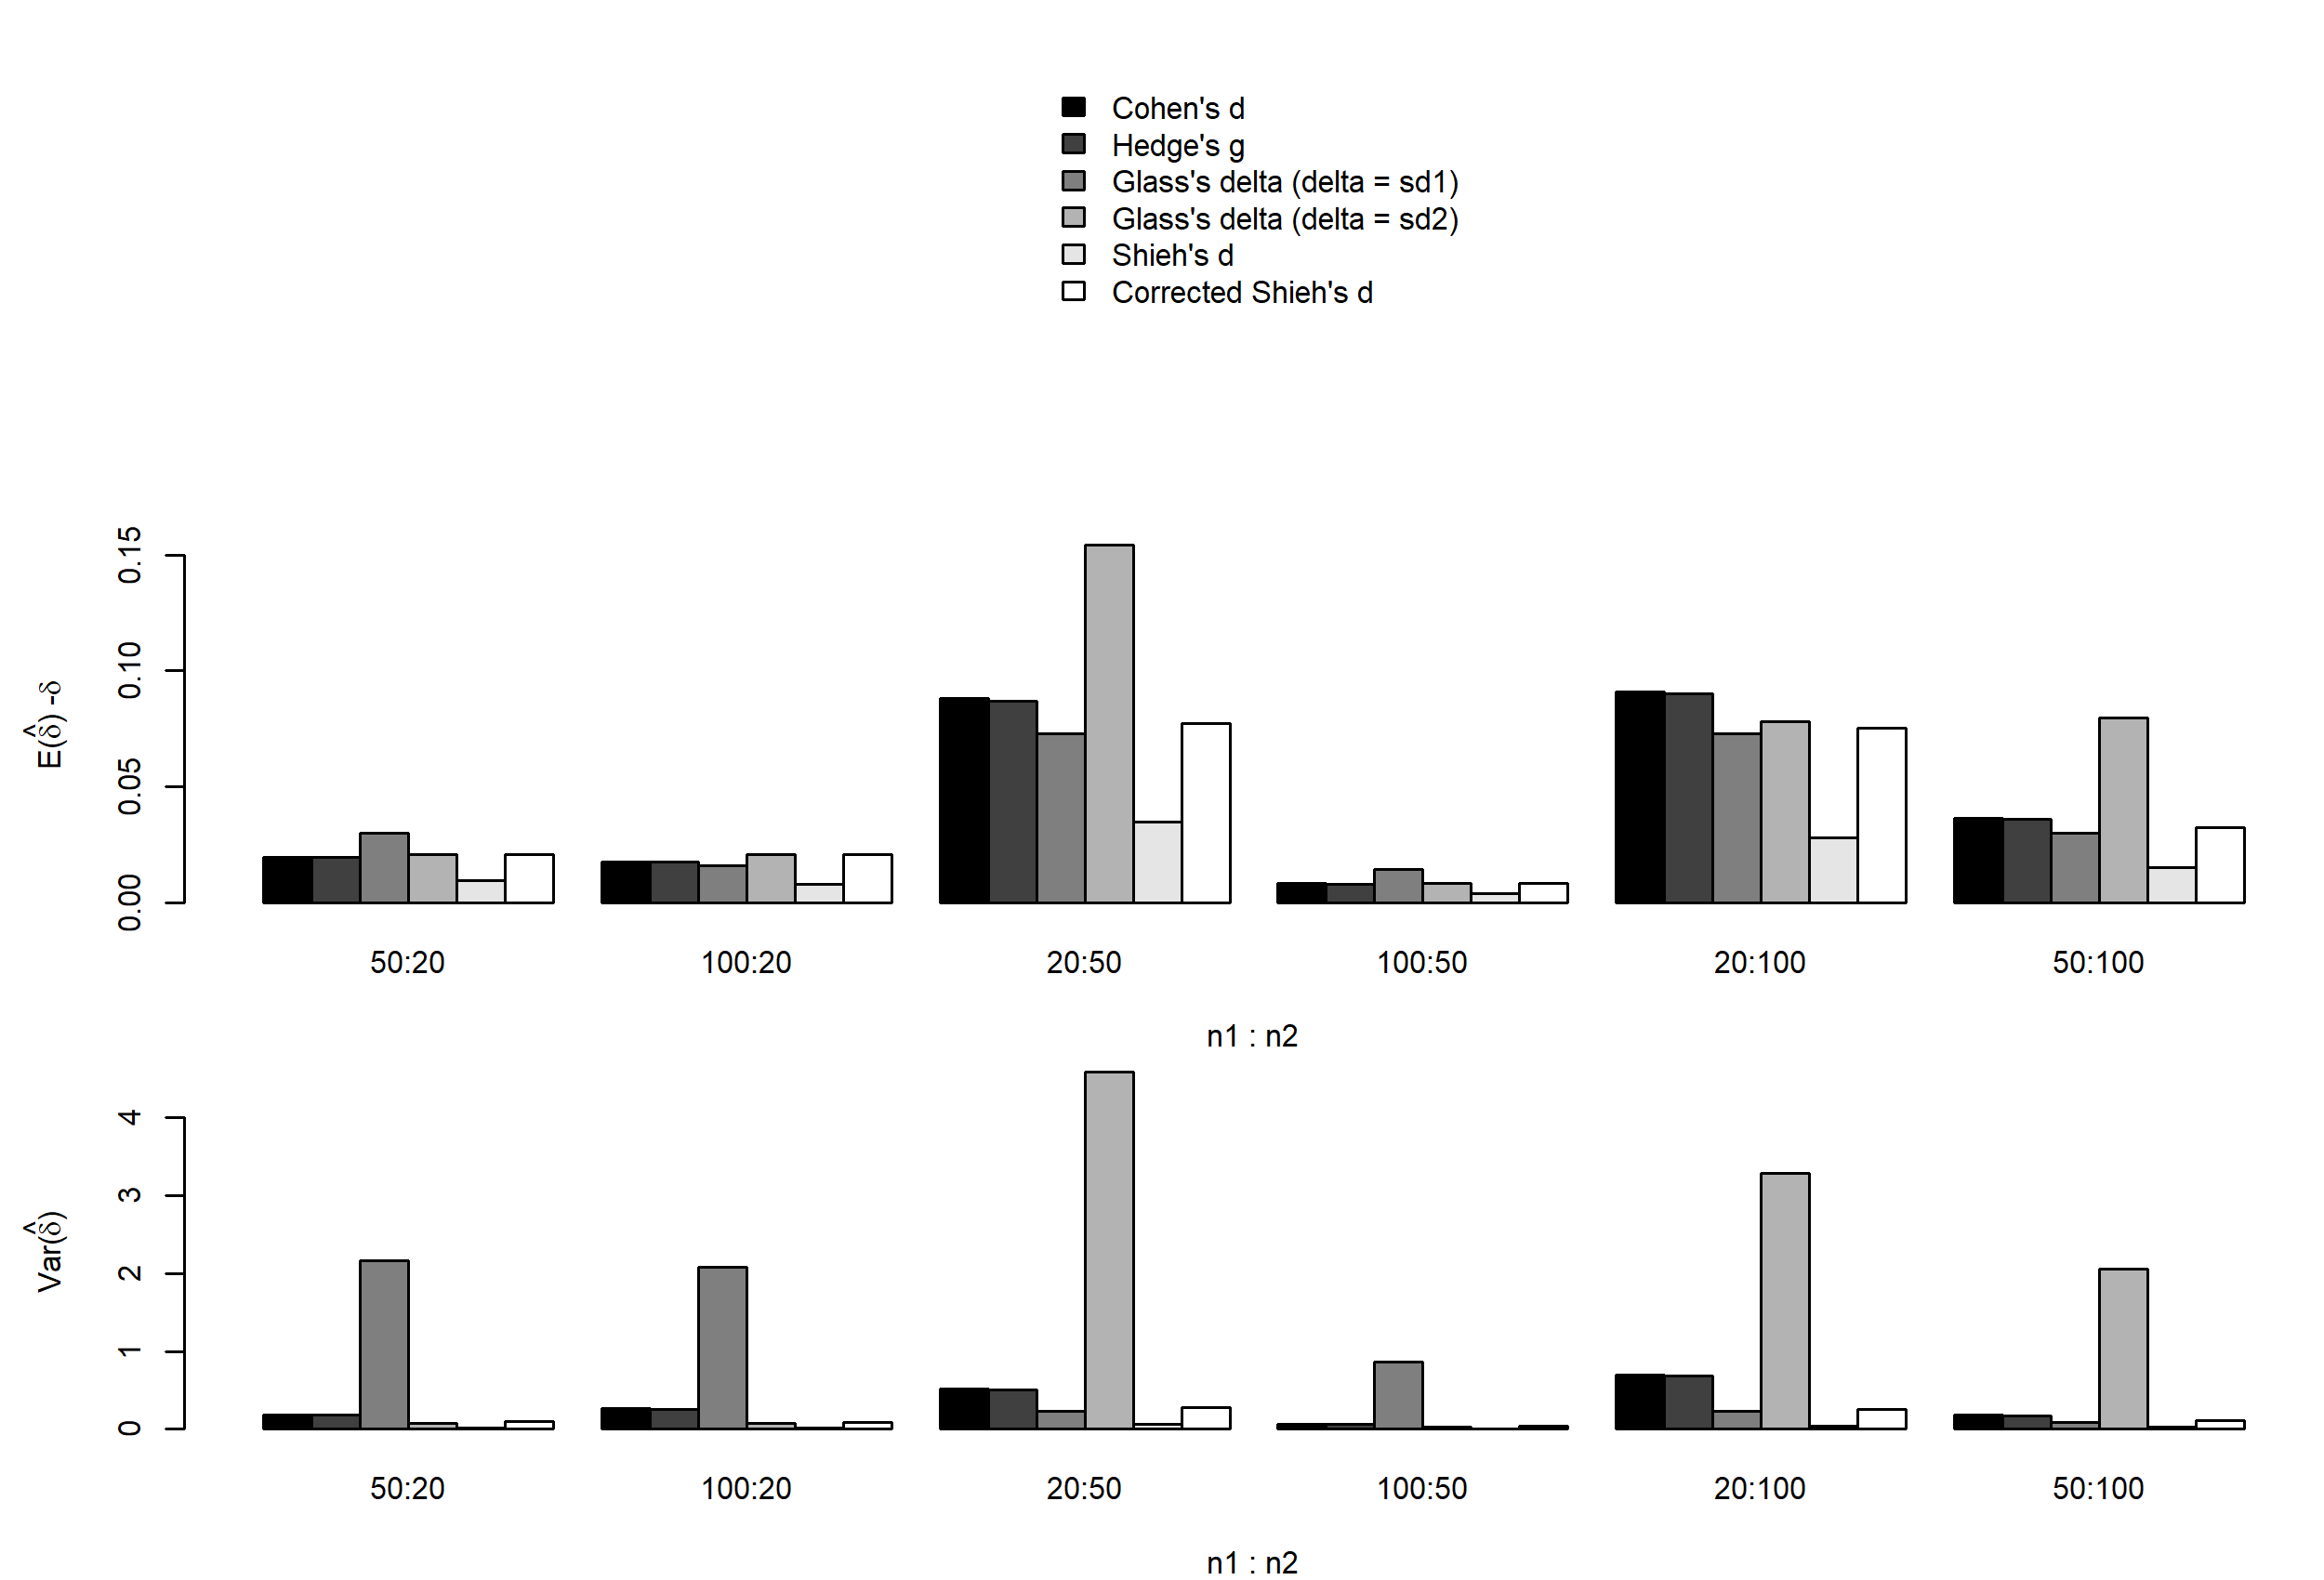
\includegraphics[width=0.2\linewidth]{C:/Users/Marie/Documents/Github_projects/Effect-sizes/Scripts outputs/Quality of ES measures/Graphs/id_Het_rneg/bias_eff,G1=0 & G2=0;id_Het_rneg} 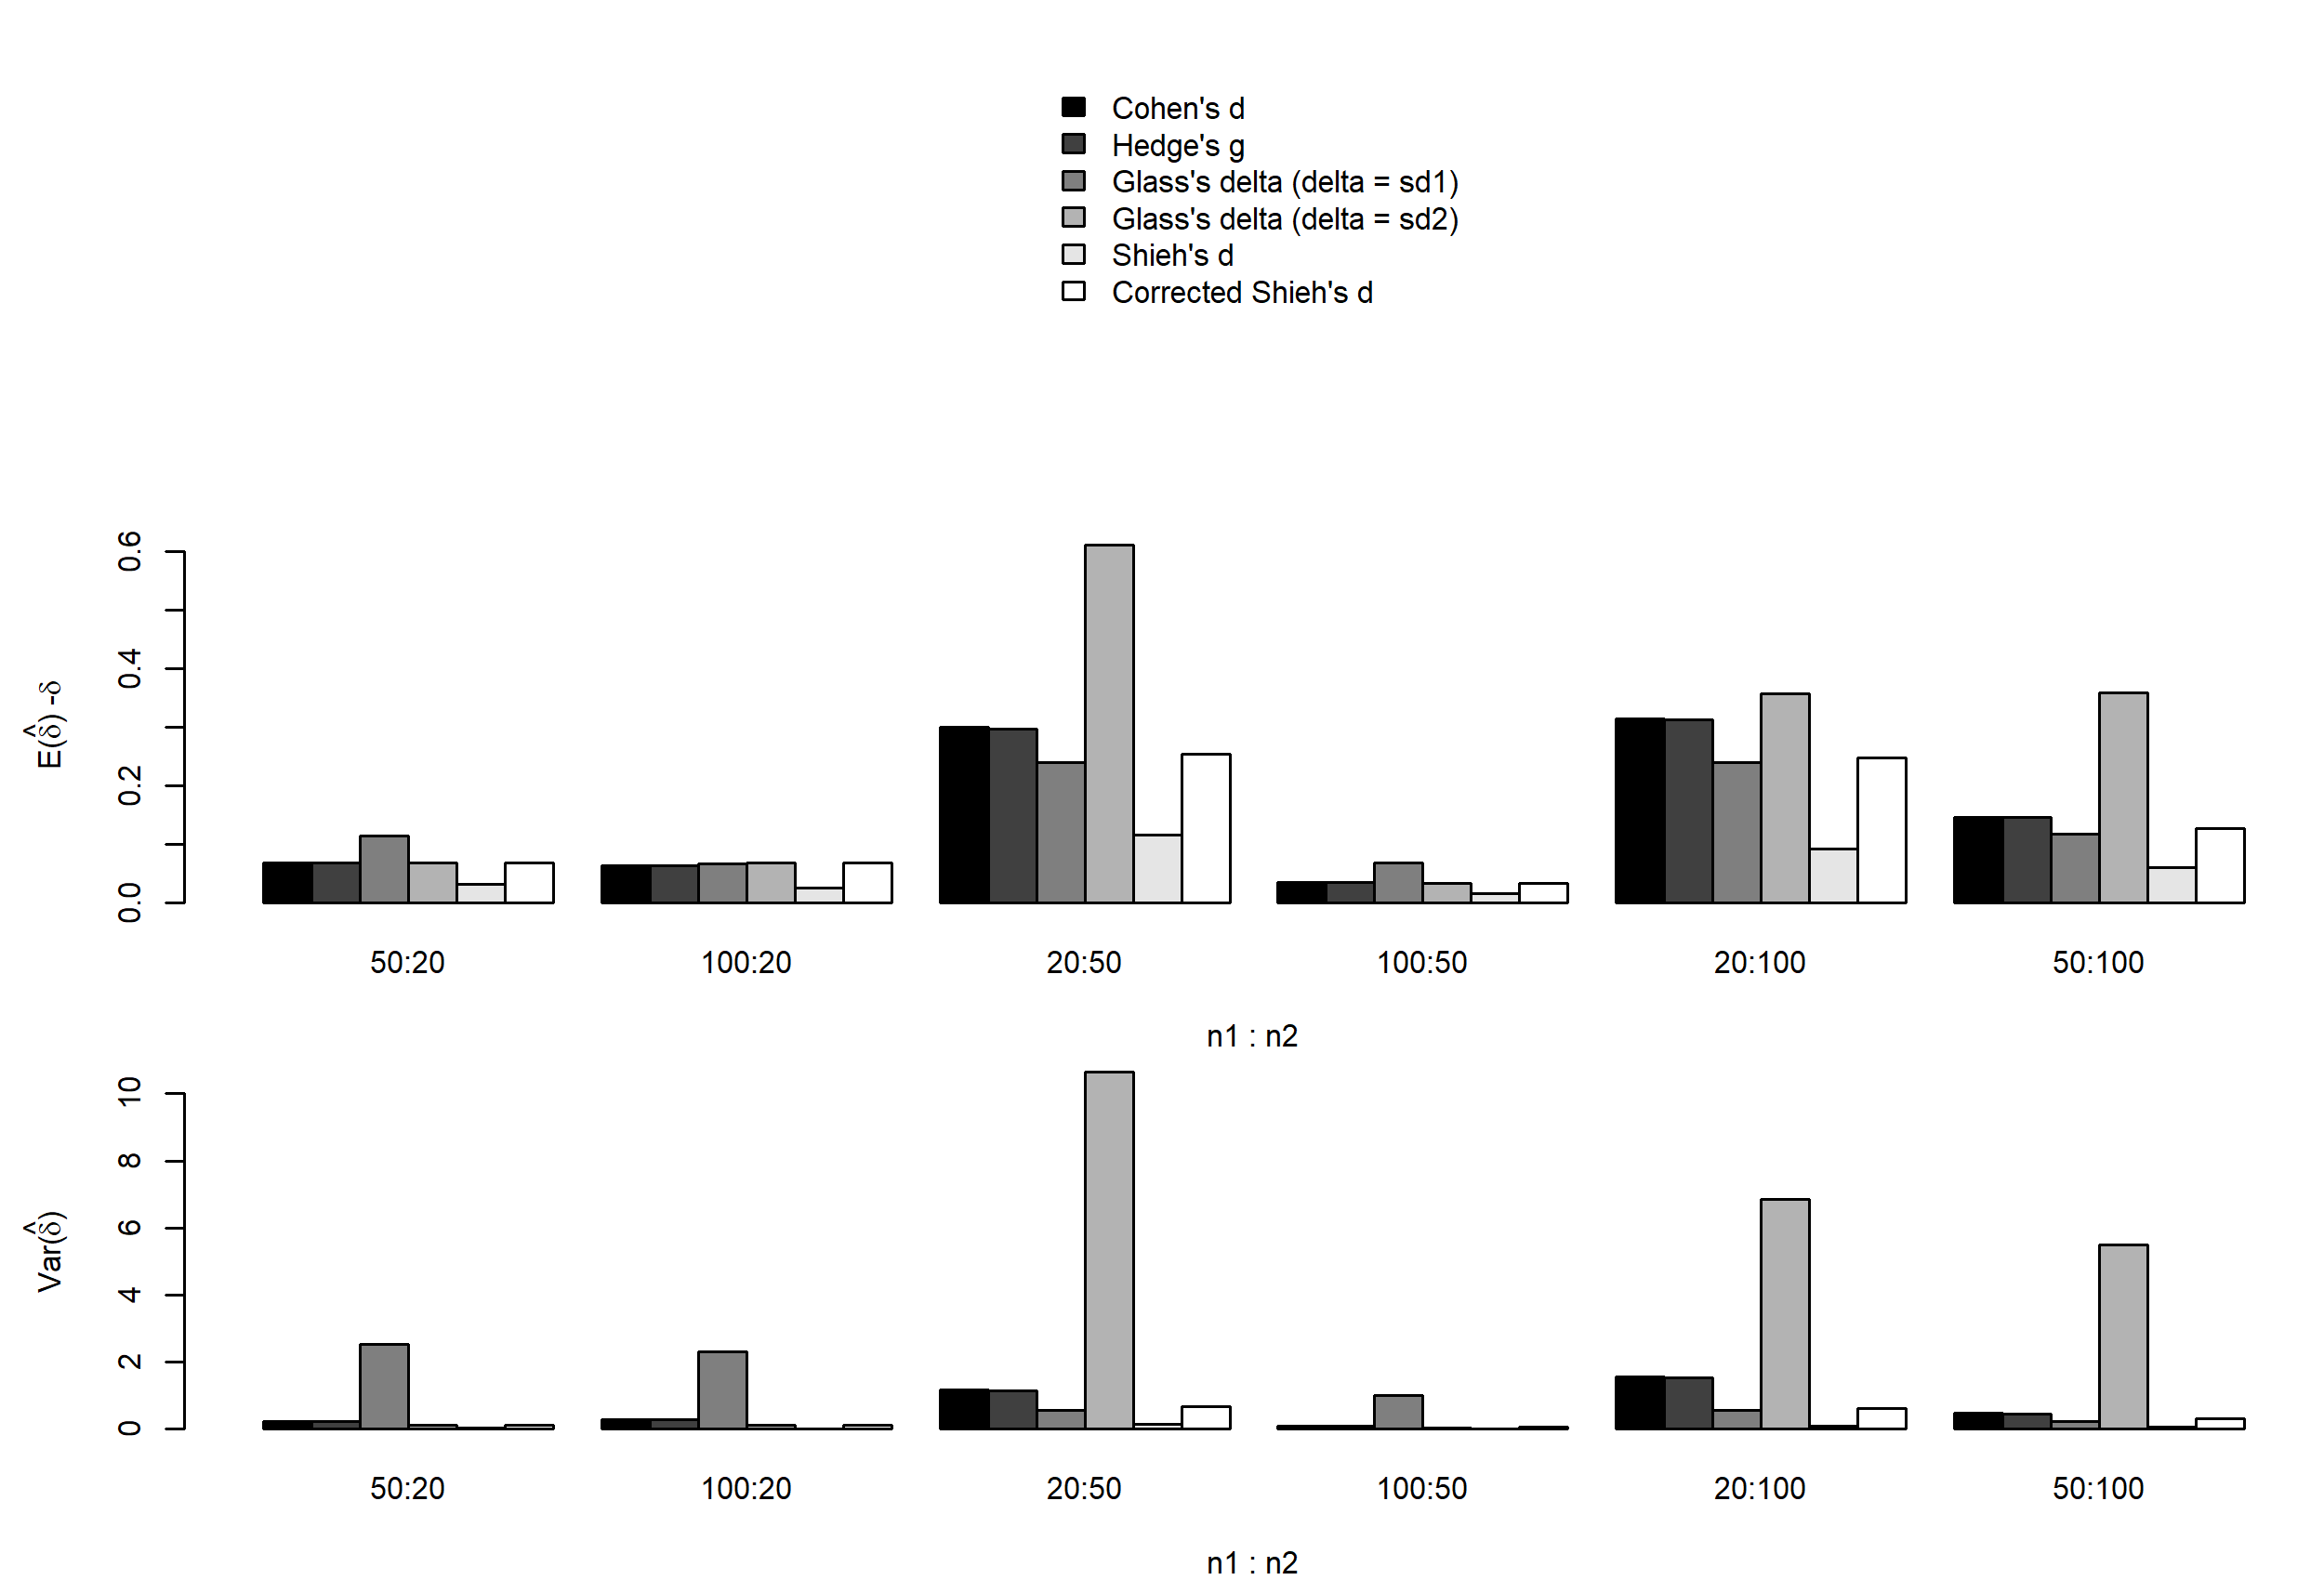
\includegraphics[width=0.2\linewidth]{C:/Users/Marie/Documents/Github_projects/Effect-sizes/Scripts outputs/Quality of ES measures/Graphs/id_Het_rneg/bias_eff,G1=0 & G2=95.75;id_Het_rneg} 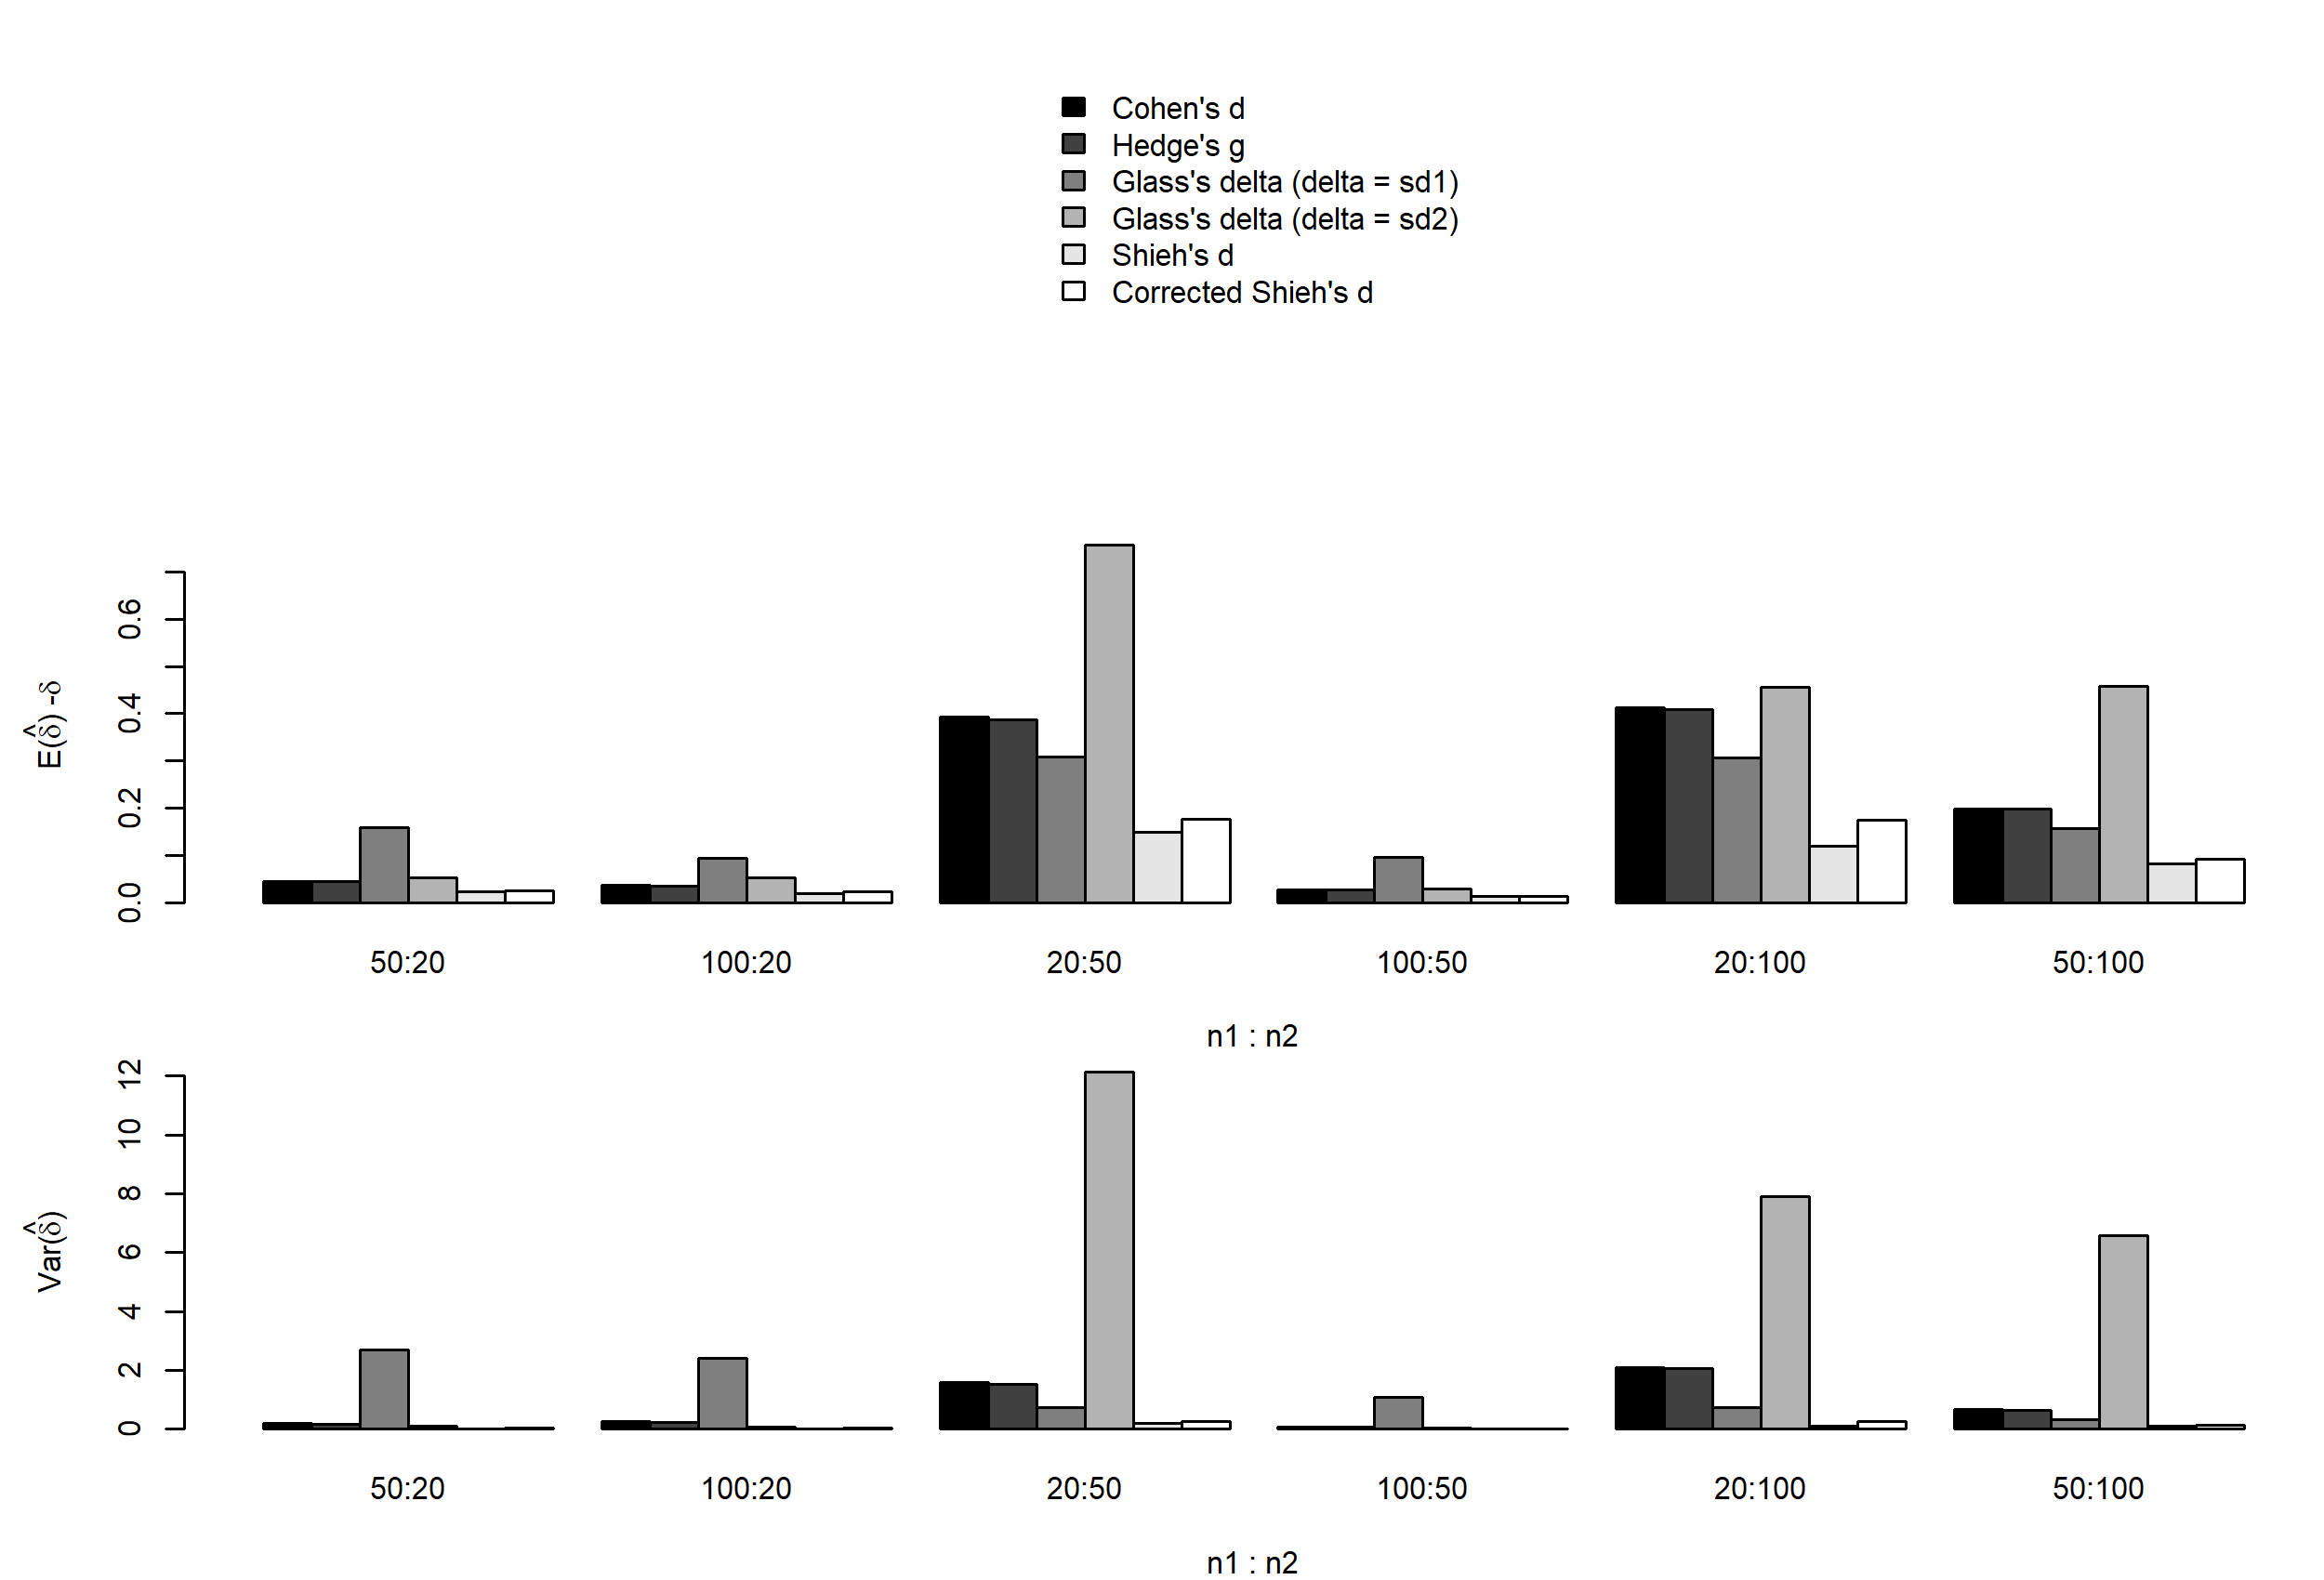
\includegraphics[width=0.2\linewidth]{C:/Users/Marie/Documents/Github_projects/Effect-sizes/Scripts outputs/Quality of ES measures/Graphs/id_Het_rneg/bias_eff,G1=2.08 & G2=95.75;id_Het_rneg} 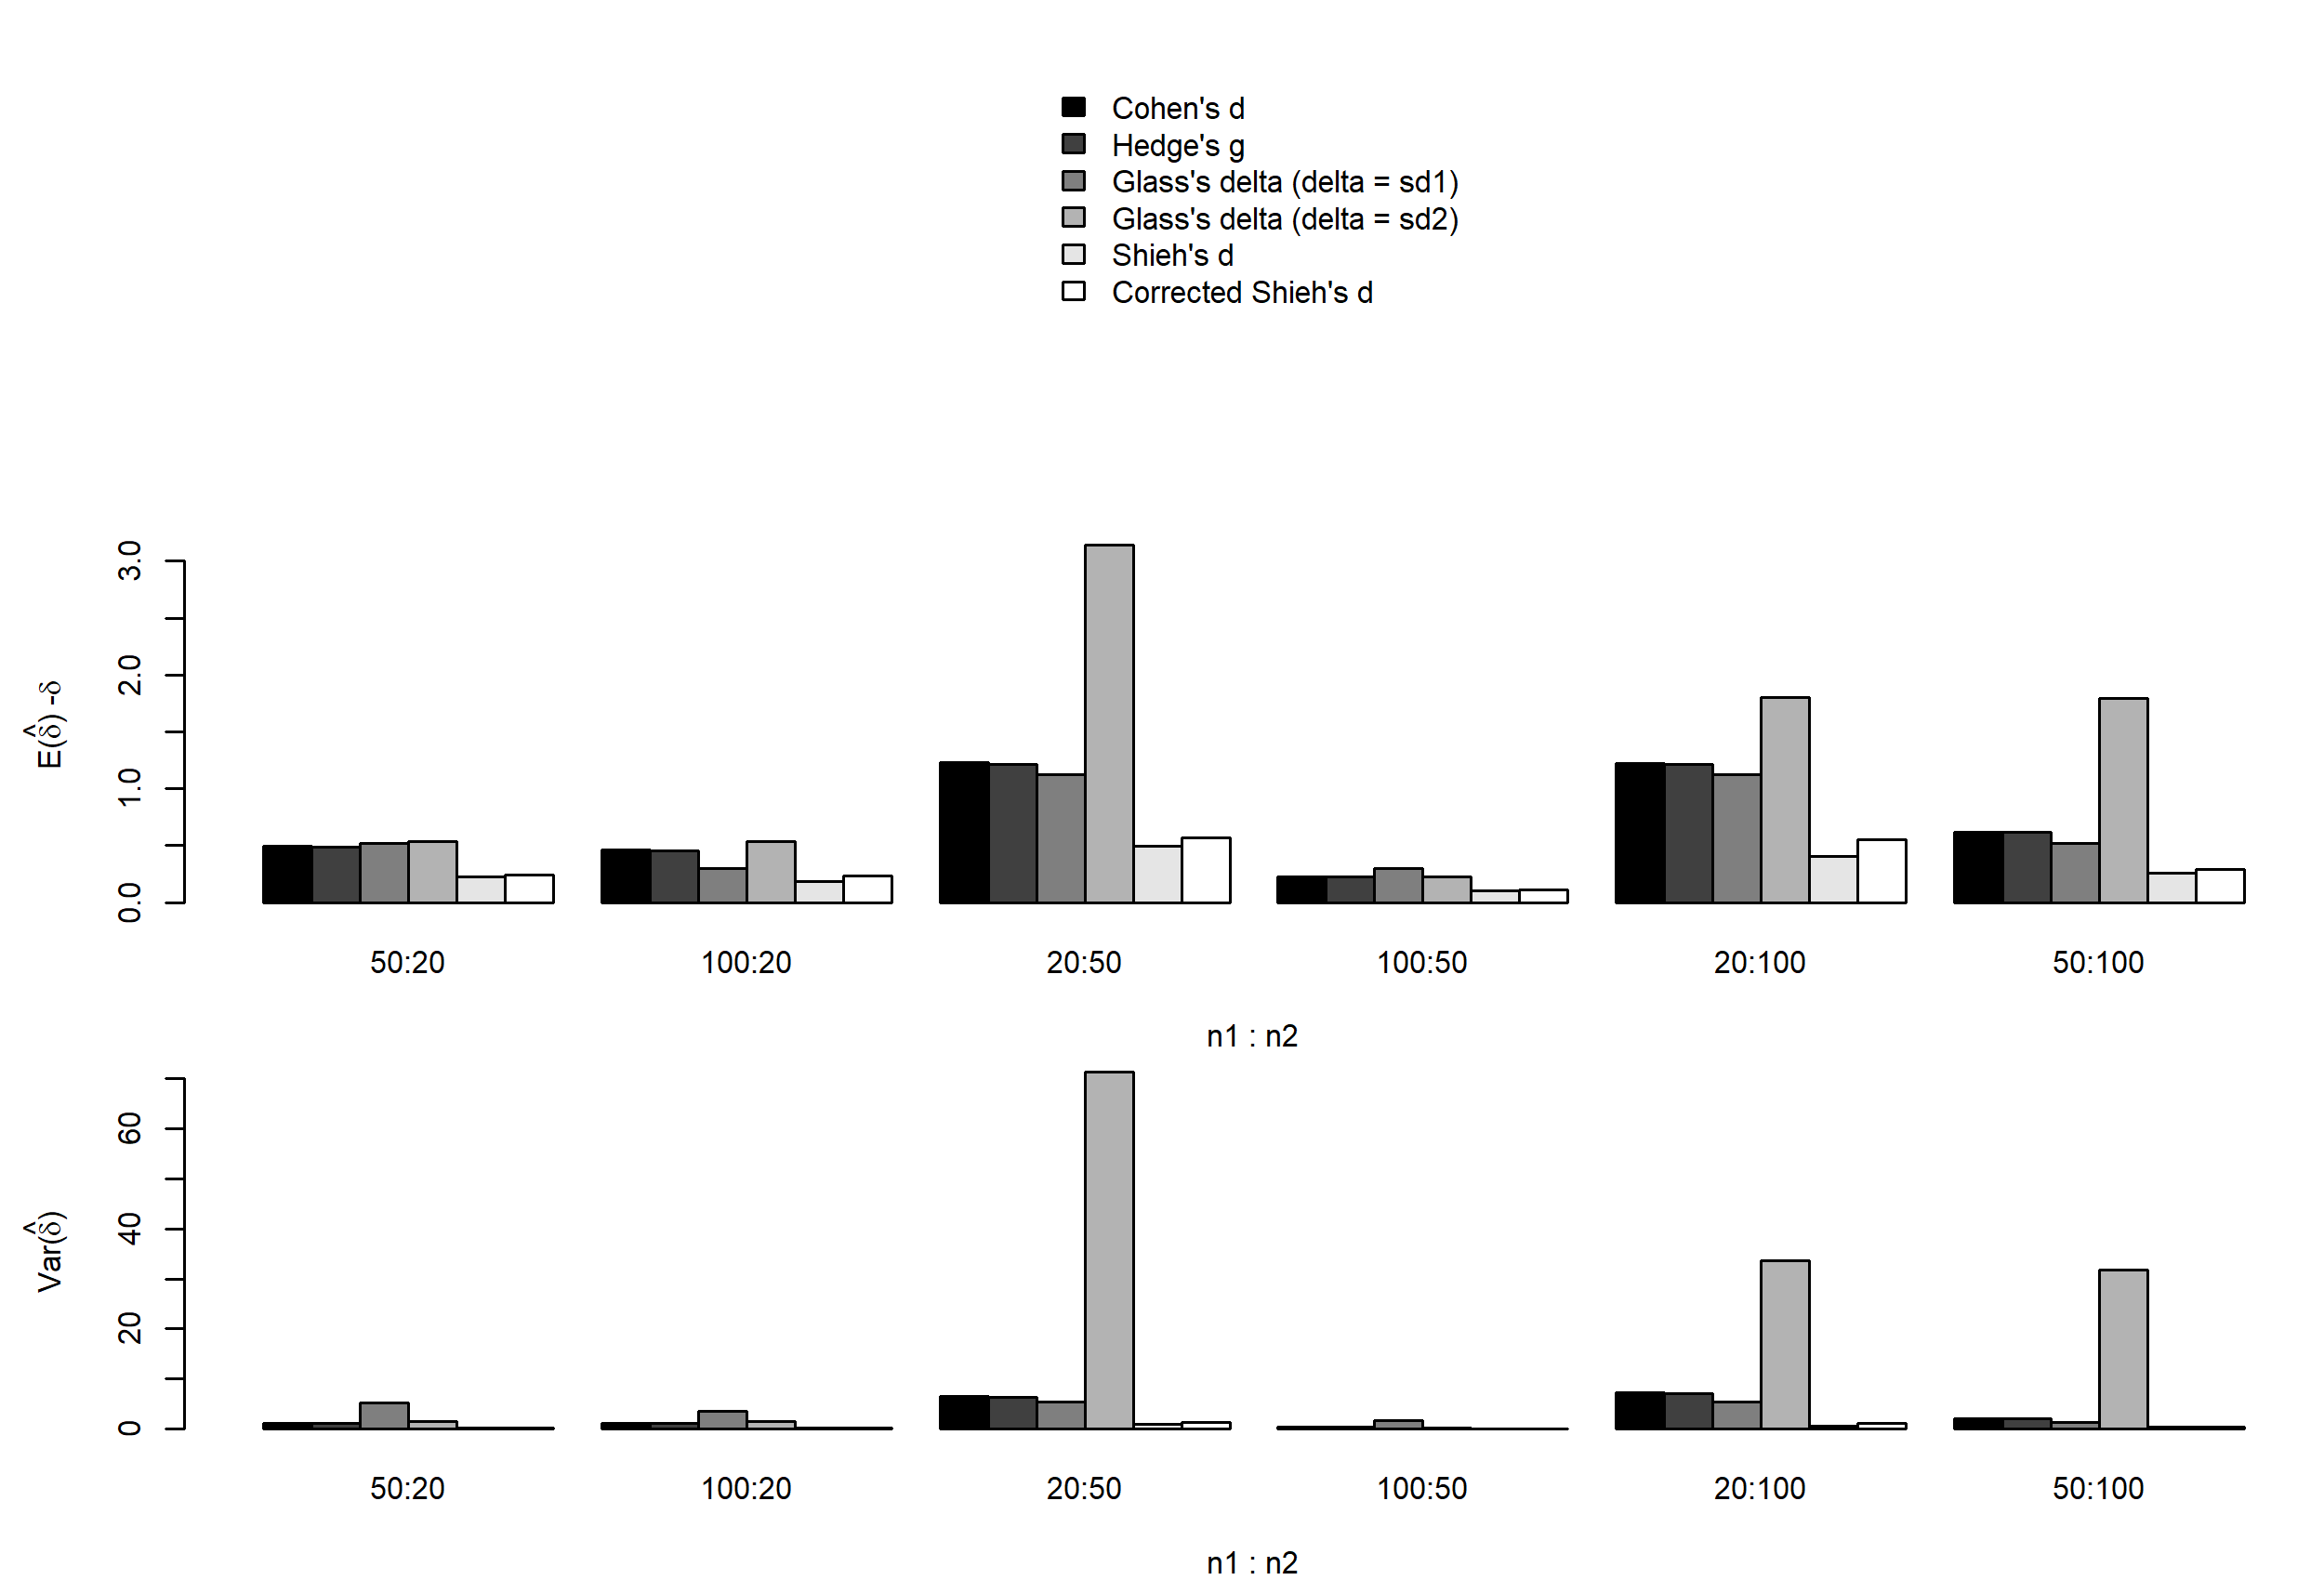
\includegraphics[width=0.2\linewidth]{C:/Users/Marie/Documents/Github_projects/Effect-sizes/Scripts outputs/Quality of ES measures/Graphs/id_Het_rneg/bias_eff,G1=6.32 & G2=95.75;id_Het_rneg} 

}

\caption{Bias and efficiency of five estimator of standardized mean difference, when variances and sample sizes are unequal across groups, with negative correlation between them}\label{fig:idHetrneg}
\end{sidewaysfigure}

In summary, Cohen's \(d_s\) and Hedge's \(d_s\) remain the best measure when the asssumption of equal variances is met. When variances are unequal across populations, Cohen's \(d_s\) and Hedge's \(g_s\) perform exactly as well as Shieh's \(d_s\) and transformed Shieh's \(d^*_s\), as long as sample sizes are equal across groups. However, when variances and sample sizes are both unequal across groups, Cohen's \(d_s\) and Hedge's \(g_s\) become irrelevant. Glass's \(d_s\) is most of the time the more biased and variable measure. We presume this could be explained by the estimation of the \(SD\) based on a subsample, because the bias is larger when standardizer is estimated based on the smallest group. Only under very specific conditions (when there is a negative correlation between sample sizes and variances and the sample size of the control group is larger than the sample size of the experimental group), Glass's \(d_s\) performs the best in comparison with all other estimators.

\begin{center}\rule{0.5\linewidth}{0.5pt}\end{center}

\hypertarget{variations-as-a-function-of-the-mean-difference}{%
\section{Variations as a function of the mean difference:}\label{variations-as-a-function-of-the-mean-difference}}

For ALL conditions,
- When distributions are symmetric

---the larger the mean difference, the larger the bias,

HOWEVER, the relative bias is constant for all mean differences

---the larger the mean difference, the larger the variance: relativement faible (surtout pour Shieh et trahsformed Shieh's) SAUF pour le glass sous certaine conditions (là ça devient plus marqué):
--\textgreater{} si on prend comme standardiseur le plus petit n
--\textgreater{} si on prend comme standardiseur le plus petit sd
--\textgreater{} Les deux facteurs semblent jouer de la même manière puisqu'on trouve à peu près les memes ratios pour Het\_bal, Hom\_rnull et Het\_rneg. Par contre, leur effet peut se cumuler, car le cas où on trouve les ratios les plus élevés, c'est Het\_rpos quand on prend simultanément le plus petit n avec le plus petit sd.

Détail: à nouveau on dirait que c'est pire quand sd2 est pris mais c'est dû à la note de bas de page de l'article (quand sd1 est le plus petit, il faut toujours 1. ALors que quand sd2 est le plus petit, il peut descendre jusque .1).

HOWEVER, the larger the mean difference, the LOWER the relative variance (pas vraiment de différence entre les estimateurs, les droites sont //). Le ratio est surtout élevé quand il y a hétéroscédasticité, surtout quand sdratio = .1 (donc exactement le contraire que pour la variance).

\begin{itemize}
\tightlist
\item
  When distributions are skewed (à voir quand j'aurai compris les bizarreries avec Christophe)
\end{itemize}

\hypertarget{variations-as-a-function-of-the-sdratio-uxe0-faire}{%
\section{Variations as a function of the sdratio (à faire):}\label{variations-as-a-function-of-the-sdratio-uxe0-faire}}

\hypertarget{conclusion}{%
\paragraph{Conclusion}\label{conclusion}}

SUMMARY GLASS: il y a 2 facteurs \enquote{aggravants} quand distribution symétriques, et 3 facteurs \enquote{aggravants} quand distributions asymétriques:\\
- SD calculé sur base du plus petit n (--\textgreater{} mesure plus variable et biaisée car distributions plus asymétrique)\\
- SD négativement corrélé avec la différence de moyenne quand mu1-mu2 \textgreater{} 0 (= choix de SD2 quand asymétrie positive, et de SD1 quand asymétrie négative, vu qu'on calcule m1-m2) OU SD positivement corrélé avec la différence de moyenne quand mu1-mu2 \textless{} 0 (= choix de SD1 quand asymétrie positive, et de SD2 quand asymétrie négative, vu qu'on calcule m1-m2).\\
- sigma? -\textgreater{} reste à voir!

Shieh's \(d_s\) and our transformed Shieh's \(d^*_S\) are the only measure that have an acceptable bias and variance in all configurations. Considering the fact that our transformed Shieh's \(d^*_s\) is much more generalizable (and therefore interpretable) than Shieh \(d_s\), we would recommend the use of this measure in all situations, unless we have very good reason to believe that variances are the same across populations.

\hypertarget{simulation-2-confidence-intervals}{%
\subsubsection{Simulation 2: confidence intervals}\label{simulation-2-confidence-intervals}}

VOIR SI ON GARDE OU PAS.
\#\#\#\# Method
\#\#\# Results
\#\#\#\# Conclusion

\hypertarget{refs}{}
\leavevmode\hypertarget{ref-Altman_2005}{}%
Altman, G. D. (2005). Why we need confidence intervals. \emph{World Journal of Surgery}, \emph{29}, 554--556. doi:\href{https://doi.org/10.1007/s00268-005-7911-0}{10.1007/s00268-005-7911-0}

\leavevmode\hypertarget{ref-AERA_2006}{}%
American Educational Research Association. (2006). Standards for reporting on empirical social science research in aera publications. \emph{Educational Researcher}, \emph{35}, 33--40. doi:\href{https://doi.org/10.3102/0013189X035006033}{10.3102/0013189X035006033}

\leavevmode\hypertarget{ref-APA_2010}{}%
American Psychological Association. (2010). \emph{Publication manual of the american psychological association {[}apa{]} (6 ed.)} (American Psychological Association.). Washington, DC:

\leavevmode\hypertarget{ref-Andersen_et_al_2007}{}%
Andersen, M. B., McCullagh, P., \& Wilson, G. J. (2007). But what do the numbers really tell us? Arbitrary metrics and effect size reporting in sport psychology research. \emph{Journal of Sport \& Exercise Psychology}, \emph{29}, 664--672.

\leavevmode\hypertarget{ref-Bothe_Richardson_2011}{}%
Bothe, A. K., \& Richardson, J. D. (2011). Statistical, practical, clinical, and personal significance: Definitions and applications in speech-language pathology. \emph{American Journal of Speech-Language Pathology}, \emph{20}, 233--242.

\leavevmode\hypertarget{ref-Cain_et_al_2017}{}%
Cain, M. K., Zhang, Z., \& Yuan, K.-H. (2017). Univariate and multivariate skewness and kurtosis for measuring nonnormality: Prevalence, influence and estimation. \emph{Behavior Research Methods}, \emph{49}(5), 1716--1735. doi:\href{https://doi.org/10.3758/s13428-016-0814-1}{10.3758/s13428-016-0814-1}

\leavevmode\hypertarget{ref-Coe_2002}{}%
Coe, R. (2002). \emph{It's the effect size, stupid. What effect size is and why it is important}. Retrieved from \url{https://www.leeds.ac.uk/educol/documents/00002182.htm}

\leavevmode\hypertarget{ref-Cohen_1965}{}%
Cohen, J. (1965). Some statistical issues in psychological research. In \emph{Handbook of clinical psychology} (B. B. Wolman., pp. 95--121). New York: McGraw-Hill.

\leavevmode\hypertarget{ref-Cohen_1988}{}%
Cohen, J. (1988). \emph{Statistical power analysis for the behavioral sciences} (Routledge Academic.). New York, NY.

\leavevmode\hypertarget{ref-Cumming_2013}{}%
Cumming, G. (2013). Cohen's d needs to be readily interpretable: Comment on shieh (2013). \emph{Behavior Research Methods}, \emph{45}, 968--971. doi:\href{https://doi.org/10.3758/s13428-013-0392-4}{10.3758/s13428-013-0392-4}

\leavevmode\hypertarget{ref-Delacre_et_al_2017}{}%
Delacre, M., Lakens, D., \& Leys, C. (2017). Why psychologists should by default use welch's t-test instead of student's t-test. \emph{International Review of Social Psychology}, \emph{30}(1), 92--101. doi:\href{https://doi.org/10.5334/irsp.82}{10.5334/irsp.82}

\leavevmode\hypertarget{ref-Delacre_et_al_2019}{}%
Delacre, M., Leys, C., Mora, Y. L., \& Lakens, D. (2019). Taking parametric assumptions seriously: Arguments for the use of welch's f-test instead of the classical f-test in one-way anova. \emph{International Review of Social Psychology}, \emph{32}(1), 1--12. doi:\href{https://doi.org/http://doi.org/10.5334/irsp.198}{http://doi.org/10.5334/irsp.198}

\leavevmode\hypertarget{ref-Ellis_2015}{}%
Ellis, P. D. (2015). \emph{The Essential Guide to Effect Sizes: Statistical Power, Meta-Analysis, and the Interpretation of Research Results} (Cambridge University Press.). Cambridge, UK.

\leavevmode\hypertarget{ref-Erceg-Hurn_Mirosevich_2008}{}%
Erceg-Hurn, D. M., \& Mirosevich, V. M. (2008). Modern robust statistical methods: An easy way to maximize the accuracy and power of your research. \emph{American Psychologist}, \emph{63}(7), 591--601. doi:\href{https://doi.org/10.1037/0003-066X.63.7.591}{10.1037/0003-066X.63.7.591}

\leavevmode\hypertarget{ref-Fan_2001}{}%
Fan, X. (2001). Statistical significance and effect size in education research: Two sides of a coin. \emph{Journal of Educational Research}, \emph{94}(5), 275--282. doi:\href{https://doi.org/10.1080/00220670109598763}{10.1080/00220670109598763}

\leavevmode\hypertarget{ref-Glass_et_al_1981}{}%
Glass, G. V., McGav, B., \& Smith, M. L. (2005). \emph{Meta-analysis in social research} (Sage.). Beverly Hills, CA.

\leavevmode\hypertarget{ref-Glass_et_al_1972}{}%
Glass, G. V., Peckham, P. D., \& Sanders, J. R. (1972). Consequences of failure to meet assumptions underlying the fixed effects analyses of variance and covariance. \emph{Review of Educational Research}, \emph{42}(3), 237--288. doi:\href{https://doi.org/10.3102/00346543042003237}{10.3102/00346543042003237}

\leavevmode\hypertarget{ref-Grissom_2000}{}%
Grissom, R. J. (2000). Heterogeneity of variance in clinical data. \emph{Journal of Consulting and Clinical Psychology}, \emph{68}(1), 155--165. doi:\href{https://doi.org/10.1037//0022-006x.68.1.155}{10.1037//0022-006x.68.1.155}

\leavevmode\hypertarget{ref-Grissom_Kim_2001}{}%
Grissom, R. J., \& Kim, J. J. (2001). Review of assumptions and problems in the appropriate conceptualization of effect size. \emph{Psychological Methods}, \emph{6}(2), 135--146. doi:\href{https://doi.org/10.1037/1082-989X.6.2.135}{10.1037/1082-989X.6.2.135}

\leavevmode\hypertarget{ref-Grissom_and_kim_2005}{}%
Grissom, R. R., \& Kim, J. J. (2005). \emph{Effect size for research: A broad practical approach.} (Lawrence Erlbaum Associates, Mahwah, N.J.). London.

\leavevmode\hypertarget{ref-Hays_1963}{}%
Hays, W. L. (1963). \emph{Statistics for psychologists} (Holt, Rinehart \& Winston.). New York.

\leavevmode\hypertarget{ref-Hedges_1981}{}%
Hedges, L. V. (1981). Distribution theory for glass's estimator of effect size and related estimators. \emph{Journal of Educational Statistics}, \emph{6}(2), 107--128.

\leavevmode\hypertarget{ref-Hedges_Olkin_1985}{}%
Hedges, L. V., \& Olkin, I. (1985). \emph{Statistical methods for meta-analysis} (Academic Press.). Cambridge, Massachusetts. doi:\href{https://doi.org/10.1016/C2009-0-03396-0}{10.1016/C2009-0-03396-0}

\leavevmode\hypertarget{ref-Henson_Smith_2000}{}%
Henson, R. I., \& Smith, A. D. (2000). State of the art in statistical significance and effect size reporting: A review of the APA task force report and current trends. \emph{Journal of Research and Development in Education}, \emph{33}(4), 285--296.

\leavevmode\hypertarget{ref-Kelley_2005}{}%
Kelley, K. (2005). The effects of nonnormal distributions on confidence intervales around the standardized mean difference: Bootstrap and parametric confidence intervals. \emph{Educational and Psychological Measurement}, \emph{65}(1), 51--69. doi:\href{https://doi.org/10.1177/0013164404264850}{10.1177/0013164404264850}

\leavevmode\hypertarget{ref-Kirk_2009}{}%
Kirk, R. E. (2009). Practical significance: A concept whose time has come. \emph{Educational and Psychological Measurement}, \emph{56}(5), 746--759. doi:\href{https://doi.org/10.1177/0013164496056005002\%20}{10.1177/0013164496056005002 }

\leavevmode\hypertarget{ref-Lakens_2013}{}%
Lakens, D. (2013). Calculating and reporting effect sizes to facilitate cumulative science: A practical primer for t-tests and ANOVAs. \emph{Frontiers in Psychology}, \emph{4}(863), 1--12. doi:\href{https://doi.org/10.3389/fpsyg.2013.00863}{10.3389/fpsyg.2013.00863}

\leavevmode\hypertarget{ref-Li_2016}{}%
Li, J. (2016). Effect size measures in a two-independent-samples case with nonnormal and nonhomogeneous data. \emph{Behavior Research Methods}, \emph{48}(4), 1560--1574. doi:\href{https://doi.org/10.3758/s13428-015-0667-z}{10.3758/s13428-015-0667-z}

\leavevmode\hypertarget{ref-McBride_et_al_1993}{}%
McBride, G. B., Loftis, J. C., \& Adkins, N. C. (1993). What do significance tests really tell us about the environment? \emph{Environmental Management}, \emph{17}(4), 423--432.

\leavevmode\hypertarget{ref-Meehl_1990}{}%
Meehl, P. E. (1990). Appraising and amending theories: The strategy of Lakatosian defense and two principles that warrant it. \emph{Psychological Inquiry}, \emph{1}(2), 108--141.

\leavevmode\hypertarget{ref-Micceri_1989}{}%
Micceri, T. (1989). The unicorn, the normal curve, and other improbable creatures. \emph{Psychological Bulletin}, \emph{105}(1), 156--166. doi:\href{https://doi.org/10.1037/0033-2909.105.1.156}{10.1037/0033-2909.105.1.156}

\leavevmode\hypertarget{ref-Nakagawa_and_Cuthill_2007}{}%
Nakagawa, S., \& Cuthill, I. C. (2007). Effect size, confidence interval and statistical significance: A practical guide for biologists. \emph{Biological Reviews}, \emph{82}, 591--605. doi:\href{https://doi.org/10.1111/j.1469-185X.2007.00027.x}{10.1111/j.1469-185X.2007.00027.x}

\leavevmode\hypertarget{ref-Olejnik_Algina_2000}{}%
Olejnik, S., \& Algina, J. (2000). Measures of effect size for comparative studies: Applications, interpretations, and limitations. \emph{Contemporary Educational Psychology}, \emph{25}, 241--286. doi:\href{https://doi.org/10.1006/ceps.2000.1040}{10.1006/ceps.2000.1040}

\leavevmode\hypertarget{ref-Olejnik_Hess_2001}{}%
Olejnik, S., \& Hess, B. (2001). \emph{Revisiting the efficacy of glass's estimator of effect size for program impact analysis}. Retrieved from \url{https://eric.ed.gov/?id=ED452210}

\leavevmode\hypertarget{ref-Peng_and_Chen_2014}{}%
Peng, C.-Y., \& Chen, L.-T. (2014). Beyond cohen's d: Alternative effect size measures for between-subject designs. \emph{THE JOURNAL OF EXPERIMENTAL EDUCATION}, \emph{82}(1), 22--50. doi:\href{https://doi.org/10.1080/00220973.2012.745471}{10.1080/00220973.2012.745471}

\leavevmode\hypertarget{ref-Peng_et_al_2013}{}%
Peng, C.-Y., Chen, L.-T., Chiang, H.-M., \& Chiang, Y.-C. (2013). The Impact of APA and AERA Guidelines on Effect size Reporting. \emph{Contemporary Educational Psychology}, \emph{82}(1), 22--50. doi:\href{https://doi.org/10.1080/00220973.2012.745471}{10.1080/00220973.2012.745471}

\leavevmode\hypertarget{ref-Prentice_Miller_1992}{}%
Prentice, D., \& Miller, D. T. (1990). When small effects are impressive. \emph{Psychological Bulletin}, \emph{112}(1), 160--164.

\leavevmode\hypertarget{ref-Raviv}{}%
Raviv, E. (2014). \emph{Bias vs. Consistency}. Retrieved March 25, 2020, from \url{https://eranraviv.com/bias-vs-consistency/}

\leavevmode\hypertarget{ref-Rosenthal_1994}{}%
Rosenthal, R. (1994). Parametric measures of effect size. In H. Cooper \& L. V. Hedges (Eds.), \emph{The hand-book of research synthesis} (pp. 231--244). New-York: Sage.

\leavevmode\hypertarget{ref-Shieh_2013}{}%
Shieh, G. (2013). Confidence intervals and sample size calculations for the weighted eta-squared effect sizes in one-way heteroscedastic ANOVA. \emph{Behavior Research Methods}, \emph{45}(1), 2--37. doi:\href{https://doi.org/10.3758/s13428-012-0228-7}{10.3758/s13428-012-0228-7}

\leavevmode\hypertarget{ref-Steyn_2000}{}%
Steyn, H. S. (2000). Practical significance of the difference in means. \emph{Journal of Industrial Psychology}, \emph{26}(3), 1--3.

\leavevmode\hypertarget{ref-Stout_Ruble_1995}{}%
Stout, D. D., \& Ruble, T. L. (1995). Assessing the practical signficance of empirical results in accounting education research: The use of effect size information. \emph{Journal of Accounting Education}, \emph{13}(3), 281--298.

\leavevmode\hypertarget{ref-Sullivan_Feinn_2012}{}%
Sullivan, G., \& Feinn, R. (2012). Using effect size---or why the p value is not enough. \emph{Journal of Graduate Medical Education}, 279--282. doi:\href{https://doi.org/10.4300/JGME-D-12-00156.1}{10.4300/JGME-D-12-00156.1}

\leavevmode\hypertarget{ref-Wackerly_et_al_2008}{}%
Wackerly, D. D., Mendenhall, W., \& Scheaffer, R. L. (2008). \emph{Mathematical statistics with applications (7th edition)} (Brooks/Cole, Cengage Learning.). Belmont, USA.

\leavevmode\hypertarget{ref-Wilkinson_1999}{}%
Wilkinson, L., \& the Task Force on Statistical Inference. (1999). Statistical methods in psychology journals: Guidelines and explanations. \emph{American Psychologist}, \emph{54}(8), 594--604.

\leavevmode\hypertarget{ref-Yuan_et_al_2004}{}%
Yuan, K.-H., Bentler, P. M., \& Chan, W. (2004). Structural equation modeling with heavy tailed distributions. \emph{Psychometrika}, \emph{69}(3), 421--436. doi:\href{https://doi.org/10.1007/bf02295644}{10.1007/bf02295644}

\leavevmode\hypertarget{ref-Keselman_et_al_2008}{}%
(n.d.).

\leavevmode\hypertarget{ref-Altman_2005}{}%
Altman, G. D. (2005). Why we need confidence intervals. \emph{World Journal of Surgery}, \emph{29}, 554--556. doi:\href{https://doi.org/10.1007/s00268-005-7911-0}{10.1007/s00268-005-7911-0}

\leavevmode\hypertarget{ref-AERA_2006}{}%
American Educational Research Association. (2006). Standards for reporting on empirical social science research in aera publications. \emph{Educational Researcher}, \emph{35}, 33--40. doi:\href{https://doi.org/10.3102/0013189X035006033}{10.3102/0013189X035006033}

\leavevmode\hypertarget{ref-APA_2010}{}%
American Psychological Association. (2010). \emph{Publication manual of the american psychological association {[}apa{]} (6 ed.)} (American Psychological Association.). Washington, DC:

\leavevmode\hypertarget{ref-Andersen_et_al_2007}{}%
Andersen, M. B., McCullagh, P., \& Wilson, G. J. (2007). But what do the numbers really tell us? Arbitrary metrics and effect size reporting in sport psychology research. \emph{Journal of Sport \& Exercise Psychology}, \emph{29}, 664--672.

\leavevmode\hypertarget{ref-Bothe_Richardson_2011}{}%
Bothe, A. K., \& Richardson, J. D. (2011). Statistical, practical, clinical, and personal significance: Definitions and applications in speech-language pathology. \emph{American Journal of Speech-Language Pathology}, \emph{20}, 233--242.

\leavevmode\hypertarget{ref-Cain_et_al_2017}{}%
Cain, M. K., Zhang, Z., \& Yuan, K.-H. (2017). Univariate and multivariate skewness and kurtosis for measuring nonnormality: Prevalence, influence and estimation. \emph{Behavior Research Methods}, \emph{49}(5), 1716--1735. doi:\href{https://doi.org/10.3758/s13428-016-0814-1}{10.3758/s13428-016-0814-1}

\leavevmode\hypertarget{ref-Coe_2002}{}%
Coe, R. (2002). \emph{It's the effect size, stupid. What effect size is and why it is important}. Retrieved from \url{https://www.leeds.ac.uk/educol/documents/00002182.htm}

\leavevmode\hypertarget{ref-Cohen_1965}{}%
Cohen, J. (1965). Some statistical issues in psychological research. In \emph{Handbook of clinical psychology} (B. B. Wolman., pp. 95--121). New York: McGraw-Hill.

\leavevmode\hypertarget{ref-Cohen_1988}{}%
Cohen, J. (1988). \emph{Statistical power analysis for the behavioral sciences} (Routledge Academic.). New York, NY.

\leavevmode\hypertarget{ref-Cumming_2013}{}%
Cumming, G. (2013). Cohen's d needs to be readily interpretable: Comment on shieh (2013). \emph{Behavior Research Methods}, \emph{45}, 968--971. doi:\href{https://doi.org/10.3758/s13428-013-0392-4}{10.3758/s13428-013-0392-4}

\leavevmode\hypertarget{ref-Delacre_et_al_2017}{}%
Delacre, M., Lakens, D., \& Leys, C. (2017). Why psychologists should by default use welch's t-test instead of student's t-test. \emph{International Review of Social Psychology}, \emph{30}(1), 92--101. doi:\href{https://doi.org/10.5334/irsp.82}{10.5334/irsp.82}

\leavevmode\hypertarget{ref-Delacre_et_al_2019}{}%
Delacre, M., Leys, C., Mora, Y. L., \& Lakens, D. (2019). Taking parametric assumptions seriously: Arguments for the use of welch's f-test instead of the classical f-test in one-way anova. \emph{International Review of Social Psychology}, \emph{32}(1), 1--12. doi:\href{https://doi.org/http://doi.org/10.5334/irsp.198}{http://doi.org/10.5334/irsp.198}

\leavevmode\hypertarget{ref-Ellis_2015}{}%
Ellis, P. D. (2015). \emph{The Essential Guide to Effect Sizes: Statistical Power, Meta-Analysis, and the Interpretation of Research Results} (Cambridge University Press.). Cambridge, UK.

\leavevmode\hypertarget{ref-Erceg-Hurn_Mirosevich_2008}{}%
Erceg-Hurn, D. M., \& Mirosevich, V. M. (2008). Modern robust statistical methods: An easy way to maximize the accuracy and power of your research. \emph{American Psychologist}, \emph{63}(7), 591--601. doi:\href{https://doi.org/10.1037/0003-066X.63.7.591}{10.1037/0003-066X.63.7.591}

\leavevmode\hypertarget{ref-Fan_2001}{}%
Fan, X. (2001). Statistical significance and effect size in education research: Two sides of a coin. \emph{Journal of Educational Research}, \emph{94}(5), 275--282. doi:\href{https://doi.org/10.1080/00220670109598763}{10.1080/00220670109598763}

\leavevmode\hypertarget{ref-Glass_et_al_1981}{}%
Glass, G. V., McGav, B., \& Smith, M. L. (2005). \emph{Meta-analysis in social research} (Sage.). Beverly Hills, CA.

\leavevmode\hypertarget{ref-Glass_et_al_1972}{}%
Glass, G. V., Peckham, P. D., \& Sanders, J. R. (1972). Consequences of failure to meet assumptions underlying the fixed effects analyses of variance and covariance. \emph{Review of Educational Research}, \emph{42}(3), 237--288. doi:\href{https://doi.org/10.3102/00346543042003237}{10.3102/00346543042003237}

\leavevmode\hypertarget{ref-Grissom_2000}{}%
Grissom, R. J. (2000). Heterogeneity of variance in clinical data. \emph{Journal of Consulting and Clinical Psychology}, \emph{68}(1), 155--165. doi:\href{https://doi.org/10.1037//0022-006x.68.1.155}{10.1037//0022-006x.68.1.155}

\leavevmode\hypertarget{ref-Grissom_Kim_2001}{}%
Grissom, R. J., \& Kim, J. J. (2001). Review of assumptions and problems in the appropriate conceptualization of effect size. \emph{Psychological Methods}, \emph{6}(2), 135--146. doi:\href{https://doi.org/10.1037/1082-989X.6.2.135}{10.1037/1082-989X.6.2.135}

\leavevmode\hypertarget{ref-Grissom_and_kim_2005}{}%
Grissom, R. R., \& Kim, J. J. (2005). \emph{Effect size for research: A broad practical approach.} (Lawrence Erlbaum Associates, Mahwah, N.J.). London.

\leavevmode\hypertarget{ref-Hays_1963}{}%
Hays, W. L. (1963). \emph{Statistics for psychologists} (Holt, Rinehart \& Winston.). New York.

\leavevmode\hypertarget{ref-Hedges_1981}{}%
Hedges, L. V. (1981). Distribution theory for glass's estimator of effect size and related estimators. \emph{Journal of Educational Statistics}, \emph{6}(2), 107--128.

\leavevmode\hypertarget{ref-Hedges_Olkin_1985}{}%
Hedges, L. V., \& Olkin, I. (1985). \emph{Statistical methods for meta-analysis} (Academic Press.). Cambridge, Massachusetts. doi:\href{https://doi.org/10.1016/C2009-0-03396-0}{10.1016/C2009-0-03396-0}

\leavevmode\hypertarget{ref-Henson_Smith_2000}{}%
Henson, R. I., \& Smith, A. D. (2000). State of the art in statistical significance and effect size reporting: A review of the APA task force report and current trends. \emph{Journal of Research and Development in Education}, \emph{33}(4), 285--296.

\leavevmode\hypertarget{ref-Kelley_2005}{}%
Kelley, K. (2005). The effects of nonnormal distributions on confidence intervales around the standardized mean difference: Bootstrap and parametric confidence intervals. \emph{Educational and Psychological Measurement}, \emph{65}(1), 51--69. doi:\href{https://doi.org/10.1177/0013164404264850}{10.1177/0013164404264850}

\leavevmode\hypertarget{ref-Kirk_2009}{}%
Kirk, R. E. (2009). Practical significance: A concept whose time has come. \emph{Educational and Psychological Measurement}, \emph{56}(5), 746--759. doi:\href{https://doi.org/10.1177/0013164496056005002\%20}{10.1177/0013164496056005002 }

\leavevmode\hypertarget{ref-Lakens_2013}{}%
Lakens, D. (2013). Calculating and reporting effect sizes to facilitate cumulative science: A practical primer for t-tests and ANOVAs. \emph{Frontiers in Psychology}, \emph{4}(863), 1--12. doi:\href{https://doi.org/10.3389/fpsyg.2013.00863}{10.3389/fpsyg.2013.00863}

\leavevmode\hypertarget{ref-Li_2016}{}%
Li, J. (2016). Effect size measures in a two-independent-samples case with nonnormal and nonhomogeneous data. \emph{Behavior Research Methods}, \emph{48}(4), 1560--1574. doi:\href{https://doi.org/10.3758/s13428-015-0667-z}{10.3758/s13428-015-0667-z}

\leavevmode\hypertarget{ref-McBride_et_al_1993}{}%
McBride, G. B., Loftis, J. C., \& Adkins, N. C. (1993). What do significance tests really tell us about the environment? \emph{Environmental Management}, \emph{17}(4), 423--432.

\leavevmode\hypertarget{ref-Meehl_1990}{}%
Meehl, P. E. (1990). Appraising and amending theories: The strategy of Lakatosian defense and two principles that warrant it. \emph{Psychological Inquiry}, \emph{1}(2), 108--141.

\leavevmode\hypertarget{ref-Micceri_1989}{}%
Micceri, T. (1989). The unicorn, the normal curve, and other improbable creatures. \emph{Psychological Bulletin}, \emph{105}(1), 156--166. doi:\href{https://doi.org/10.1037/0033-2909.105.1.156}{10.1037/0033-2909.105.1.156}

\leavevmode\hypertarget{ref-Nakagawa_and_Cuthill_2007}{}%
Nakagawa, S., \& Cuthill, I. C. (2007). Effect size, confidence interval and statistical significance: A practical guide for biologists. \emph{Biological Reviews}, \emph{82}, 591--605. doi:\href{https://doi.org/10.1111/j.1469-185X.2007.00027.x}{10.1111/j.1469-185X.2007.00027.x}

\leavevmode\hypertarget{ref-Olejnik_Algina_2000}{}%
Olejnik, S., \& Algina, J. (2000). Measures of effect size for comparative studies: Applications, interpretations, and limitations. \emph{Contemporary Educational Psychology}, \emph{25}, 241--286. doi:\href{https://doi.org/10.1006/ceps.2000.1040}{10.1006/ceps.2000.1040}

\leavevmode\hypertarget{ref-Olejnik_Hess_2001}{}%
Olejnik, S., \& Hess, B. (2001). \emph{Revisiting the efficacy of glass's estimator of effect size for program impact analysis}. Retrieved from \url{https://eric.ed.gov/?id=ED452210}

\leavevmode\hypertarget{ref-Peng_and_Chen_2014}{}%
Peng, C.-Y., \& Chen, L.-T. (2014). Beyond cohen's d: Alternative effect size measures for between-subject designs. \emph{THE JOURNAL OF EXPERIMENTAL EDUCATION}, \emph{82}(1), 22--50. doi:\href{https://doi.org/10.1080/00220973.2012.745471}{10.1080/00220973.2012.745471}

\leavevmode\hypertarget{ref-Peng_et_al_2013}{}%
Peng, C.-Y., Chen, L.-T., Chiang, H.-M., \& Chiang, Y.-C. (2013). The Impact of APA and AERA Guidelines on Effect size Reporting. \emph{Contemporary Educational Psychology}, \emph{82}(1), 22--50. doi:\href{https://doi.org/10.1080/00220973.2012.745471}{10.1080/00220973.2012.745471}

\leavevmode\hypertarget{ref-Prentice_Miller_1992}{}%
Prentice, D., \& Miller, D. T. (1990). When small effects are impressive. \emph{Psychological Bulletin}, \emph{112}(1), 160--164.

\leavevmode\hypertarget{ref-Raviv}{}%
Raviv, E. (2014). \emph{Bias vs. Consistency}. Retrieved March 25, 2020, from \url{https://eranraviv.com/bias-vs-consistency/}

\leavevmode\hypertarget{ref-Rosenthal_1994}{}%
Rosenthal, R. (1994). Parametric measures of effect size. In H. Cooper \& L. V. Hedges (Eds.), \emph{The hand-book of research synthesis} (pp. 231--244). New-York: Sage.

\leavevmode\hypertarget{ref-Shieh_2013}{}%
Shieh, G. (2013). Confidence intervals and sample size calculations for the weighted eta-squared effect sizes in one-way heteroscedastic ANOVA. \emph{Behavior Research Methods}, \emph{45}(1), 2--37. doi:\href{https://doi.org/10.3758/s13428-012-0228-7}{10.3758/s13428-012-0228-7}

\leavevmode\hypertarget{ref-Steyn_2000}{}%
Steyn, H. S. (2000). Practical significance of the difference in means. \emph{Journal of Industrial Psychology}, \emph{26}(3), 1--3.

\leavevmode\hypertarget{ref-Stout_Ruble_1995}{}%
Stout, D. D., \& Ruble, T. L. (1995). Assessing the practical signficance of empirical results in accounting education research: The use of effect size information. \emph{Journal of Accounting Education}, \emph{13}(3), 281--298.

\leavevmode\hypertarget{ref-Sullivan_Feinn_2012}{}%
Sullivan, G., \& Feinn, R. (2012). Using effect size---or why the p value is not enough. \emph{Journal of Graduate Medical Education}, 279--282. doi:\href{https://doi.org/10.4300/JGME-D-12-00156.1}{10.4300/JGME-D-12-00156.1}

\leavevmode\hypertarget{ref-Wackerly_et_al_2008}{}%
Wackerly, D. D., Mendenhall, W., \& Scheaffer, R. L. (2008). \emph{Mathematical statistics with applications (7th edition)} (Brooks/Cole, Cengage Learning.). Belmont, USA.

\leavevmode\hypertarget{ref-Wilkinson_1999}{}%
Wilkinson, L., \& the Task Force on Statistical Inference. (1999). Statistical methods in psychology journals: Guidelines and explanations. \emph{American Psychologist}, \emph{54}(8), 594--604.

\leavevmode\hypertarget{ref-Yuan_et_al_2004}{}%
Yuan, K.-H., Bentler, P. M., \& Chan, W. (2004). Structural equation modeling with heavy tailed distributions. \emph{Psychometrika}, \emph{69}(3), 421--436. doi:\href{https://doi.org/10.1007/bf02295644}{10.1007/bf02295644}

\leavevmode\hypertarget{ref-Keselman_et_al_2008}{}%
(n.d.).

\clearpage
\makeatletter
\efloat@restorefloats
\makeatother


\begin{appendix}
\section{}
\setlength{\parindent}{0.0in}
\setlength{\leftskip}{0.0in}

\hypertarget{appendix-1-the-mathematical-study-of-shiehs-delta}{%
\subsection{\texorpdfstring{Appendix 1: The mathematical study of
Shieh's
\(\delta\)}{Appendix 1: The mathematical study of Shieh's \textbackslash delta}}\label{appendix-1-the-mathematical-study-of-shiehs-delta}}

Paste Appendix 1 when it will be finished

\hypertarget{appendix-2-confidence-intervals}{%
\subsection{Appendix 2: Confidence
intervals}\label{appendix-2-confidence-intervals}}

Paste Appendix 2 when it will be finished

\hypertarget{appendix-3-a-priori-power-analyses}{%
\subsection{Appendix 3: a priori power
analyses}\label{appendix-3-a-priori-power-analyses}}

Paste Appendix 3 when it will be finished (Cumming \& Finch, 2001)

\hypertarget{refs}{}
\leavevmode\hypertarget{ref-Cumming_Finch_2001}{}%
Cumming, G., \& Finch, S. (2001). A primer on the understanding, use,
and calculation of confidence intervales that are based on central and
noncentral distributions. \emph{Educational and Psychological
Measurement}, \emph{61}(532), 532--574.
\end{appendix}

\end{document}
